% Chapter Template

\chapter{Event selection and background estimation} % Main chapter title

\label{Chapter6} % Change X to a consecutive number; for referencing this chapter elsewhere, use \ref{ChapterX}

\lhead{Chapter 6. \emph{Event selection and background estimation}} % Change X to a consecutive number; this is for the header on each page - perhaps a shortened title

This chapter describes the event selection criteria used to identify $pp\rightarrow W+bb$ process necessary for the cross section measurement. The selection is focused on the leptonic decay modes of W boson, thus requiring the presence of an isolated muon or electron, missing energy, and two b-tagged jets. Reconstruction and identification of these object has been described in the previous chapter. All major backgrounds are identified using simulation and are used to get the final yields for the cross section measurement in chapter \ref{Chapter7}. 
This chapter is organized as follows. Samples used in the analysis together with a short description of simulation procedures are presented in section \ref{sec:samples}. In order to obtain good agreement between data and simulation, certain corrections are applied to take into account trigger and reconstruction efficiencies, pileup reweighing and b-tagging inefficiencies. Applied corrections are summarized in section \ref{sec:mcSF}. Signal selection criteria are listed in section \ref{sec:selection} while background sources are described in section \ref{sec:background}.     

\section{Data and Monte Carlo samples}
\label{sec:samples}
Data samples used in this analysis are consist of pp collisions at center of mass energy of 8 TeV collected with CMS experiment during 2012. After performing necessary data-quality checks, 19.8fb$^{-1}$ of data was marked as good quality for physics analysis. Selected events are required to pass one of the following triggers:
\begin{itemize}
\item Isolated muon with $p_T>24$ GeV,
\item Electron with $p_T>27$ GeV which passes some additional identification criteria as described in \ref{sec:eleID}.
\end{itemize}

\par Simulated samples for signal and background processes were obtained using Monte Carlo methods, as a part of the official 2012 CMS production campaign. Simulated samples include W+jets, Z+jets, $t\bar{t}$, single top and WZ samples. Several event generators were used to produce samples needed in the analysis:
\begin{itemize}
\item \textbf{Pythia} \cite{Sjostrand:2006za,Sjostrand:2007gs} is a multi-purpose generator which can also simulate parton shower. Pythia is able to calculate only tree-level 1$\rightarrow$2 and 2$\rightarrow$2 processes while higher orders are approximated with parton shower algorithm. Parton showering in all samples uses so called Z2 tune for modeling the underlying event \cite{Field:2010bc,Chatrchyan:2013ala}. Diboson samples were generated with Pythia event generator while W+jets, Z+jets and $t\bar{t}$ samples were produced with Madgraph and showered with Pythia.  
\item \textbf{Madgraph} \cite{Alwall:2011uj} calculates matrix elements on tree level for dercays and 2$\rightarrow n$ scatterings (with $n$ going up to 10). Radiation of hard gluons in initial and final state is taken into account on the matrix element calculation level. A minimum $p_T$ threshold is defined in order to avoid soft gluon emissions which cause total cross section to be strongly scale dependent. Thus, cross section is normalized to predictions from other software, such as MCFM\cite{Campbell:2010ff} for standard model processes.   
\item \textbf{aMC@NLO} \cite{Alwall:2014hca} automates and unifies the tree-level and next-to-leading order computation tools within the MadGraph family.
\item \textbf{Powheg} \cite{Oleari:2010nx} is a package optimized for heavy quark production in hadronic collisions. The hard process is calculated at the NLO order, but for fragmentation and hadronization other software is used (e.g. Pythia). Single top events were produced using this generator and showered with Pythia. 
\item \textbf{Tauola} \cite{Jadach:1993hs} is a package for simulation of $\tau$ decays.
\end{itemize}
        
Detector response is simulated using GEANT4 simulation package \cite{Agostinelli:2002hh}. Data was analyzed using ROOT framework \cite{Brun:1997pa}. List of the used samples together with the corresponding luminosities is listed in the Table \ref{tab:samples} except for the QCD sample which is determined using a data-driven technique described in section \ref{sec:QCD}.

\begin{table}[h]
  \centering
  \caption{Samples, generators and cross sections used for normalizations for signal and background simulation considered in this analysis. All samples are normalized to the NLO cross-section calculation except the W+jets which is NNLO and $t\bar{t}$ which is normalized to the latest combined cross section measurement of ATLAS and CMS collaborations \cite{CMS:2014gta}. }
  \label{tab:samples}
  \begin{tabular}{ l  c c}
      \hline
      \hline
      	Sample & Generator & $\sigma(pb)(NLO)$ \\
      	\hline
    		W($\rightarrow l \nu$)+jets &  Madgraph + Pythia & $37509$ (NNLO) \\
     	W $+$ 1 jet & Madgraph $+$ Pythia & $-$ \\
     	W $+$ 2 jets & Madgraph $+$ Pythia & $-$ \\
     	W $+$ 3 jets & Madgraph $+$ Pythia & $-$ \\
     	W $+$ 4 jets & Madgraph $+$ Pythia & $-$ \\
     	W $+$ bb & Madgraph $+$ Pythia & 377.4 \\
     	\hline
     	Z $+$ jets & Madgraph $+$ Pythia &  3531.9 \\     	
     	$t\bar{t}$ semi-leptonic & Madgraph $+$ Pythia &  107.7 \\
     	$t\bar{t}$ full-leptonic & Madgraph $+$ Pythia &  25.8 \\
     	\hline
     	single $t$ - t$-$channel & Powheg $+$ Pythia &  56.4 \\
     	single $t$ - s$-$channel & Powheg $+$ Pythia &  3.97 \\
		single $t$ - tW$-$channel & Powheg $+$ Pythia &  11.1 \\
		single $\bar{t}$ - t$-$channel & Powheg $+$ Pythia &  30.7 \\
		single $\bar{t}$ - s$-$channel & Powheg $+$ Pythia &  1.76 \\
		single $\bar{t}$ - tW$-$channel & Powheg $+$ Pythia &  11.1 \\
		\hline
		WZ & Pythia & 33.6 \\
		WW & Pythia & 56.0 \\
      \hline
      \hline 
  \end{tabular}
\end{table}

Signal events are simulated in exclusive W+1,2,3,4 jets samples using Madgraph event generator and showered with Pythia. These samples are generated using the five-flavour scheme with massless b-quark in the initial state. Samples are than divided into three subsamples labeled as W+b(b), W+c(c) and W+light. W+b(b) subsample is selected by the requirement that there be a generated B hadron starting with pdgId=$\pm$5 in one of the jets. W+c(c) samples is selected if c quark is generated in one of the jets (pdgId$=\pm$4). Events are classified sequentially with W+b(b) events selected first. All other events are labeled as W+light jets (W+udcsg). Additionally, analysis has been preformed using the shape from four-flavour sample listed in the Table \ref{tab:samples} which has much larger number of generated signal events. It was normalized to five-flavour cross section .

%----------------------------------------------------------------------------------------
%	SECTION 2
%----------------------------------------------------------------------------------------


\section{Monte-Carlo corrections}
\label{sec:mcSF}

\subsection{Pileup}

In proton-proton collisions at high beam intensities, there is a high probability that multiple interactions will happen in a single bunch crossing. These additional interactions are usually referred to as pileup interactions and contain low$-p_T$ QCD jets. The identification of such jets as well as their removal is described in detail in \cite{CMS:2013wea}. The total inelastic cross section in the 2012 is 69 mb, so the luminosity per bunch crossing of 69 mb$^{-1}$ results in one interaction per bunch crossing. As the instantaneous luminosity per bunch crossing was higher than the total inelastic cross section, this resulted in 21 primary interactions on the average during 2012, with some bunch crossings  going up to 70. With these conditions it is important to recognize the signature from such interactions.  
\par Simulated events have different distribution for number of pileup interaction with respect to data. This occurs because it was difficult to predict the exact pileup distribution in data during the generation of the simulated events. Therefore, simulated events were reweighed to match the distribution in data. For each simulated event, a weight $w_{PU}$ is derived based on the number of pileup events provided by the generator. Figure \ref{fig:N_pu} shows number of pile-up events before and after the reweighing procedure for signal events in the muon channel. The agreement between data and simulation has improved after the procedure which id also visible in the ratio plot. 

\begin{figure}[htbp]
	\centering
		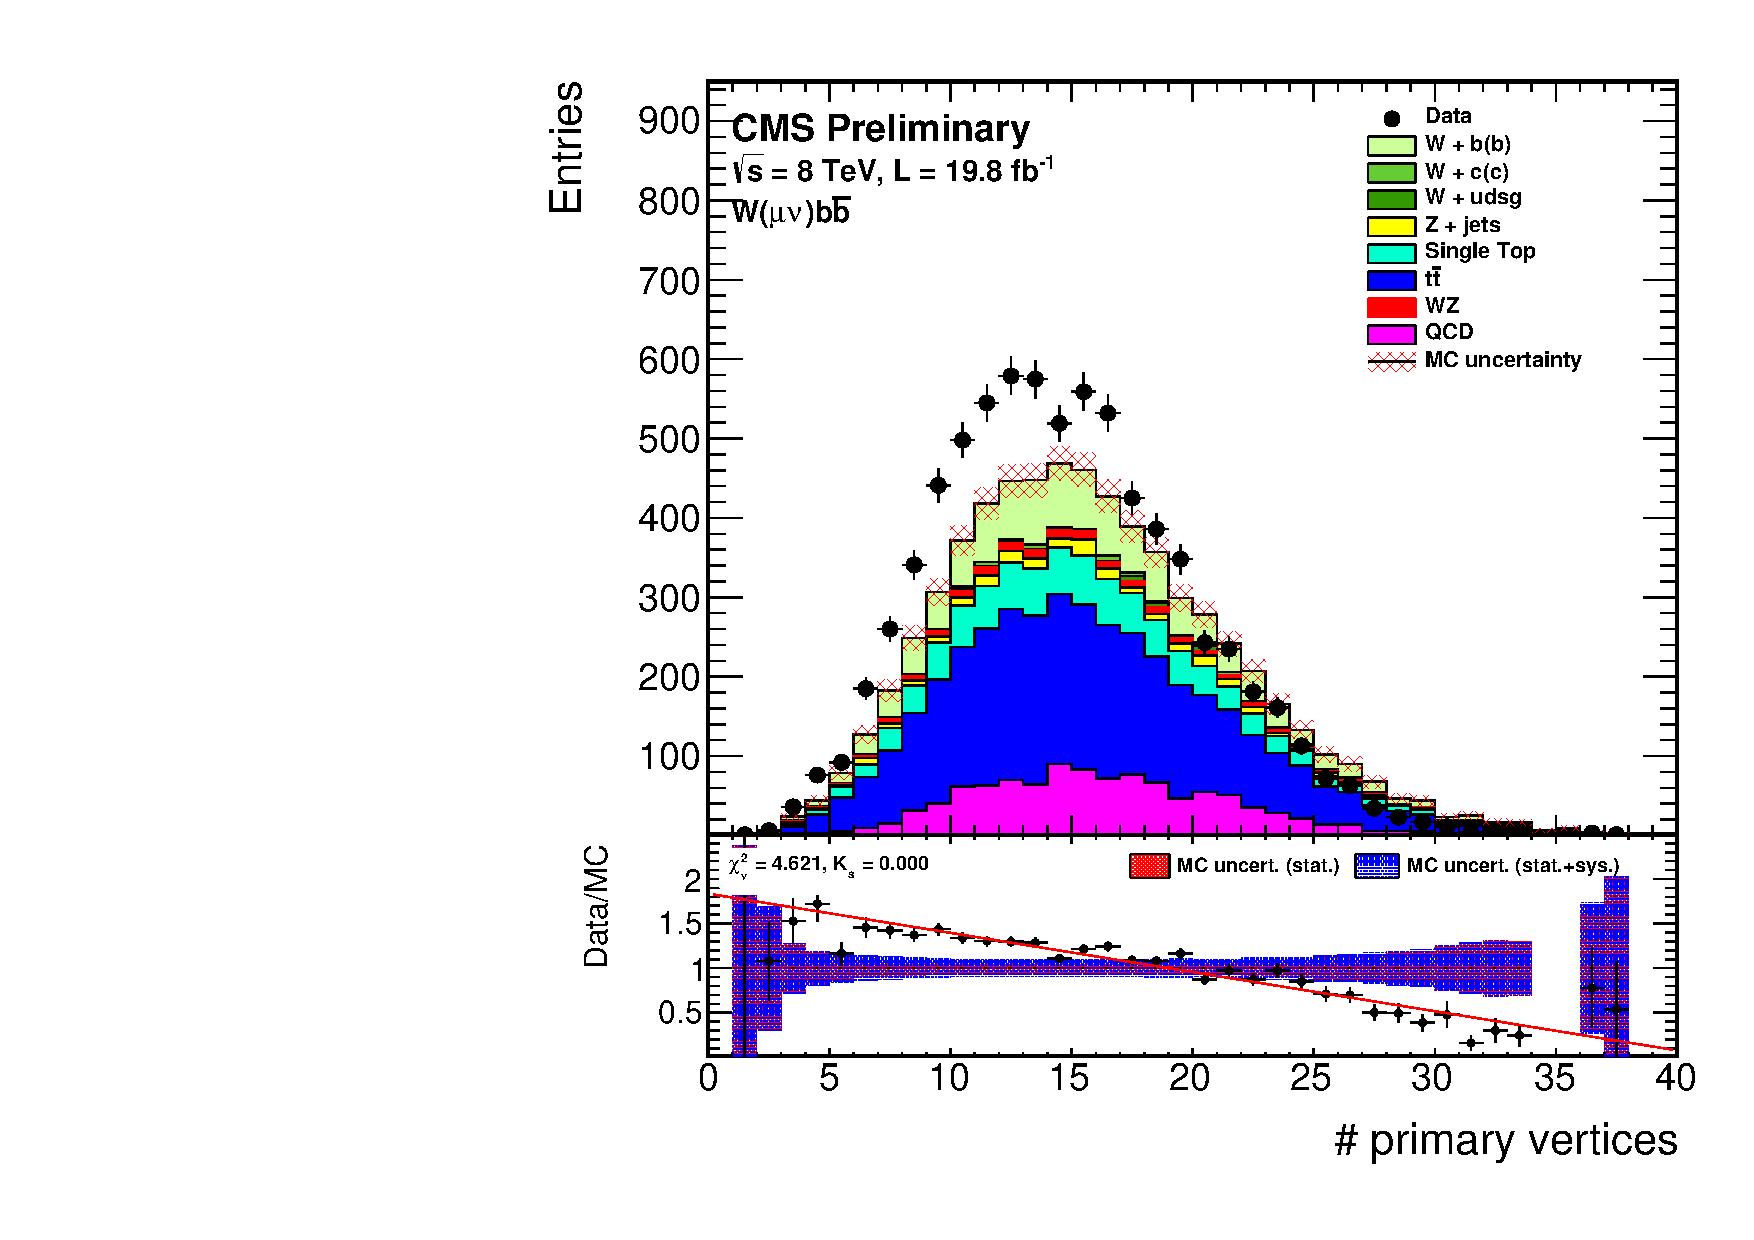
\includegraphics[width=0.48\textwidth]{Figures/Results/noPU.pdf}
		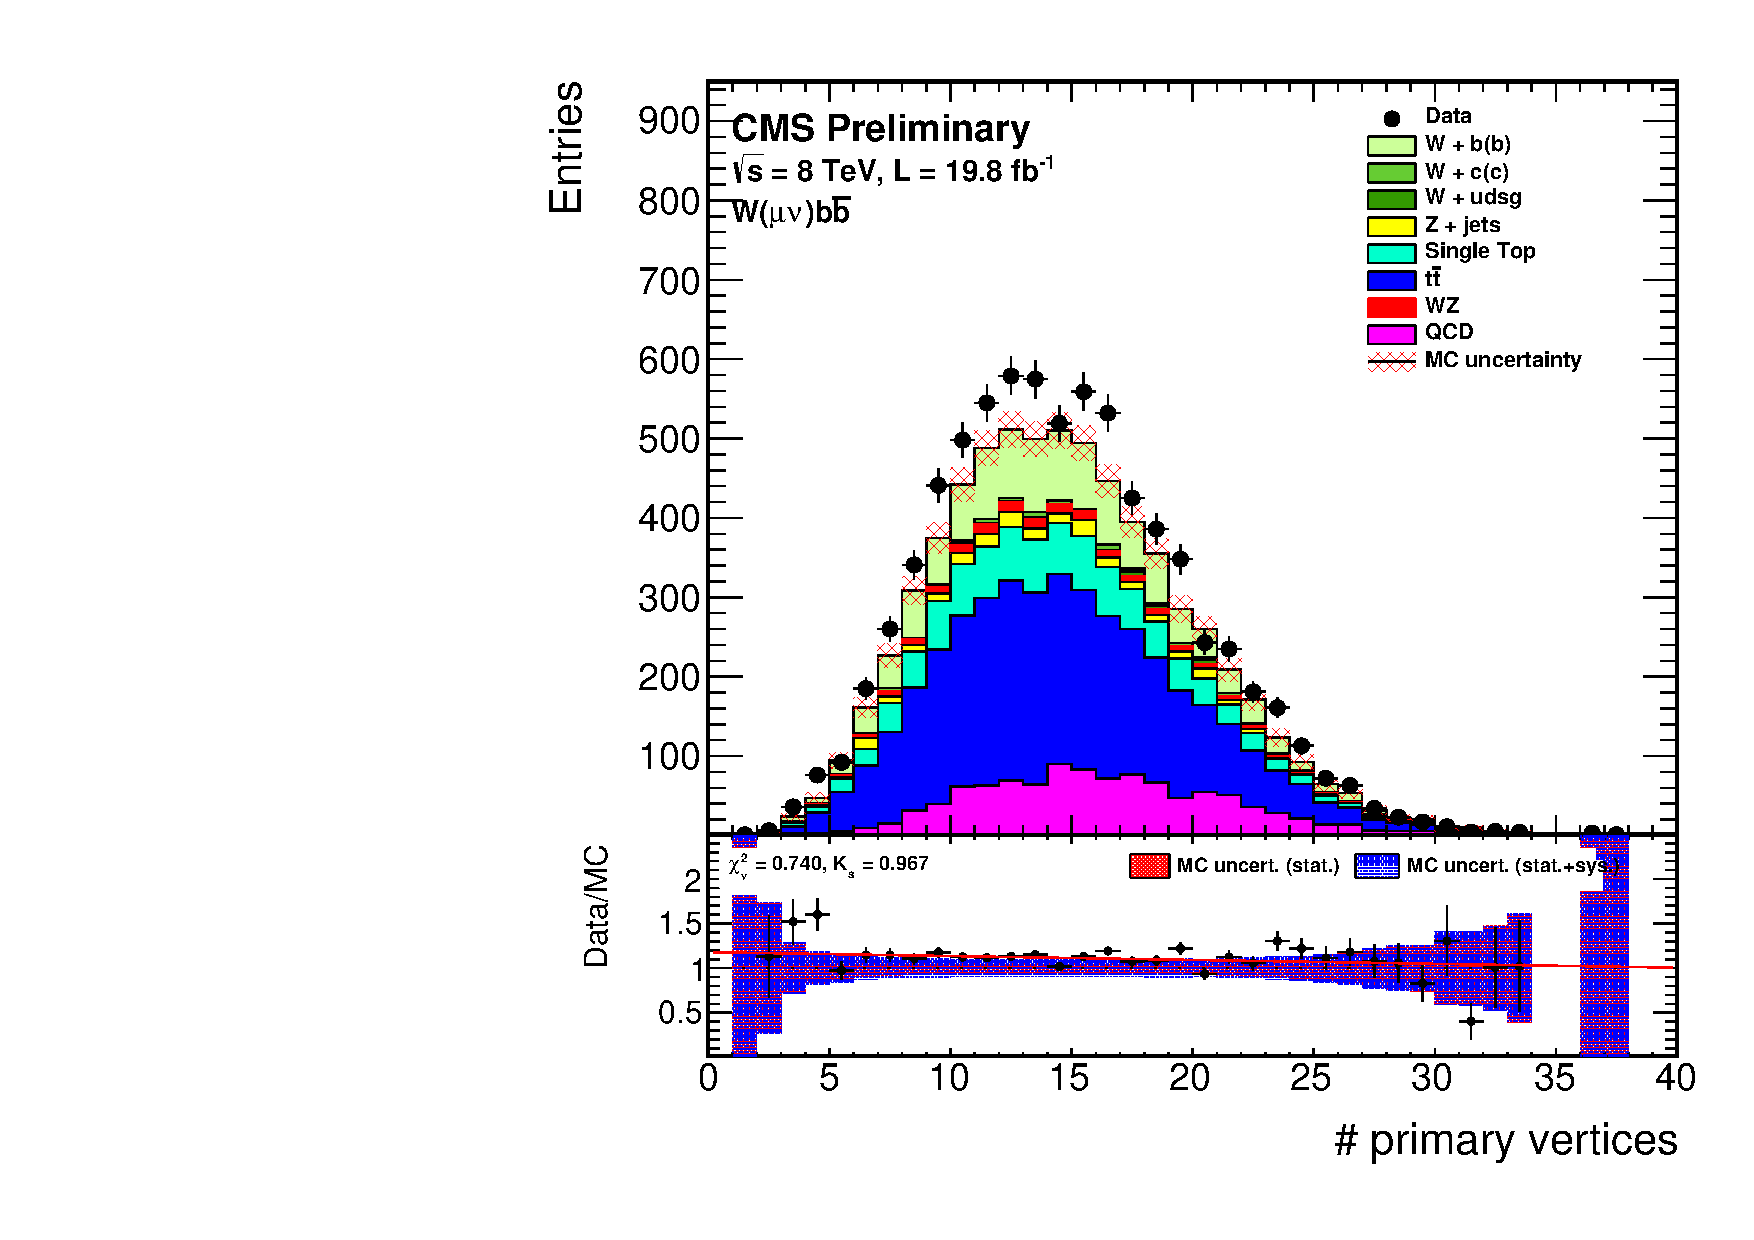
\includegraphics[width=0.48\textwidth]{Figures/Results/withPU.pdf}	
		%\rule{35em}{0.5pt}
	\caption[Number of primary vertices before and after the pileup reweighing procedure.]{Number of primary vertices before (\textit{left}) and after (\textit{right}) the pileup reweighing procedure.}
	\label{fig:N_pu}
\end{figure} 

\subsection{Lepton efficiency measurement}
\label{sec:lepEff}

Events used for cross section measurement are required to pass certain triggers in order to be selected. However, trigger selection is not 100$\%$ efficient and the selection efficiency has to be determined. The additional steps in the analysis, like reconstruction and isolation, have some inefficiencies as well. Efficiency estimation from simulation shows large systematic errors due to inaccuracy in signal modeling and detector response. This was the main motivation for development of the fully data-driven efficiency estimation called \textit{Tag and probe}. In this method, using well-known mass resonances, such as Z boson, are used and a selection criteria is applied to the decay products. 
Very tight selection criteria are applied on one Z boson daughter lepton (\textit{tag}) while the looser cuts, used in the analysis, are applied on the other (\textit{probe}) lepton. The efficiency ($\epsilon$) for certain cut is than determined by counting the number of probe leptons that pass the cut ($N_{pass}$) divided by the number of the all probe leptons. This number includes the probe leptons that passed and failed the cut ($N_{fail}$):    
\begin{equation}
\epsilon = \frac{N_{pass}}{N_{pass}+N_{fail}}
\end{equation} 
As it is not possible to uniquely identify Z bosons, while performing tag and probe method, invariant mass distributions of the two leptons are used to determine $N_{pass}$ and $N_{fail}$. 
%\textit{Tag} lepton is the one passing very tight selection cuts with low missidentification probability. The efficiency for certain cuts is than measured by counting \textit{probe} leptons which are leptons passing this looser cut divided by number of all leptons. Probes are selected in such way that the invariant mass of the two leptons falls into the Z mass resonance. The following relation is used for the measurement:
  
%Final selection contains a number of events where Z boson was not actually produced and which have to be subtracted. Both 
Signal and background are parametrized and their contributions are estimated using maximum likelihood fit. For signal events a convolution of Z shape with a Gaussian is used to take into account the detector effects, while for background parametrization, a combination of exponential function and polinomial was used.
\par The efficiency was measured as a function of pseudorapidity and transverse momentum of a passing probe. Trigger, identification and isolation criteria were used in electron and muon channels separately. Both data and Monte Carlo efficiencies were measured and their ratio was used as a scale factor for each event in order to match simulated lepton efficiencies to measured data. Muon identification and isolation efficiency for data and MC for barrel part ($|\eta|<0.9$) of the detector is shown in figure \ref{fig:eff_IDISO} while trigger efficiency measurement is shown in figure \ref{fig:eff_trig}. Similar values for the efficiencies are obtained for the other parts of the detector.

\begin{figure}[htbp]
	\centering
		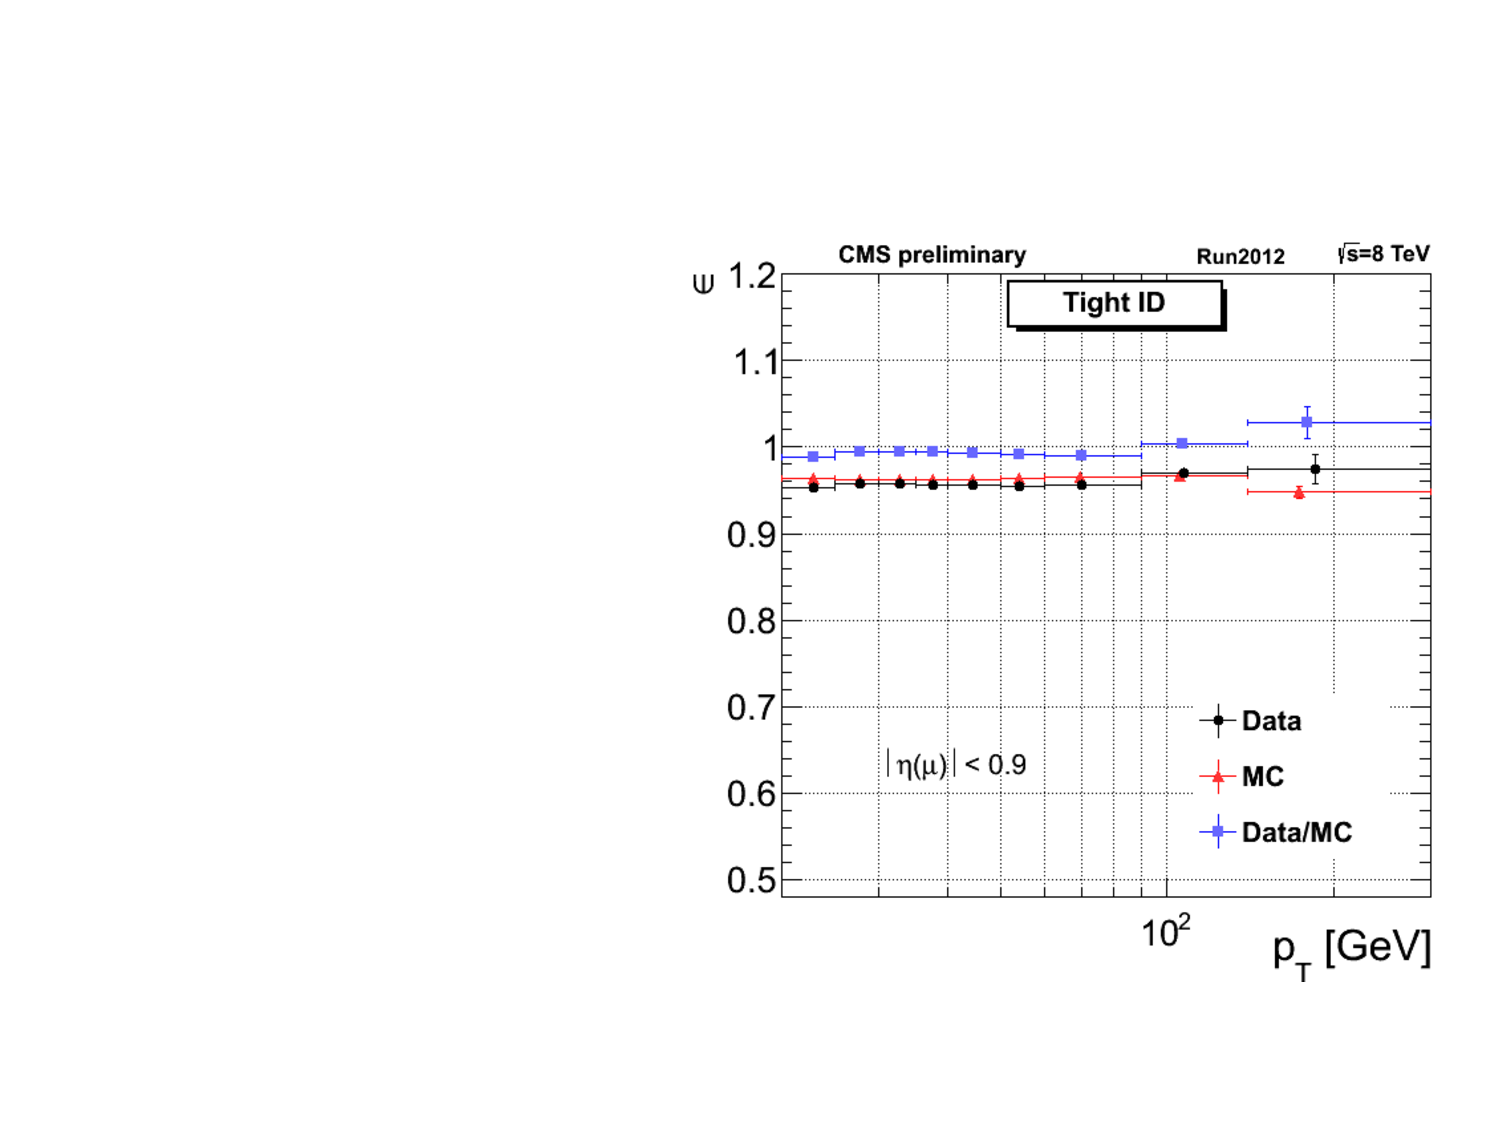
\includegraphics[width=0.49\textwidth]{Figures/ID_eff.pdf}
		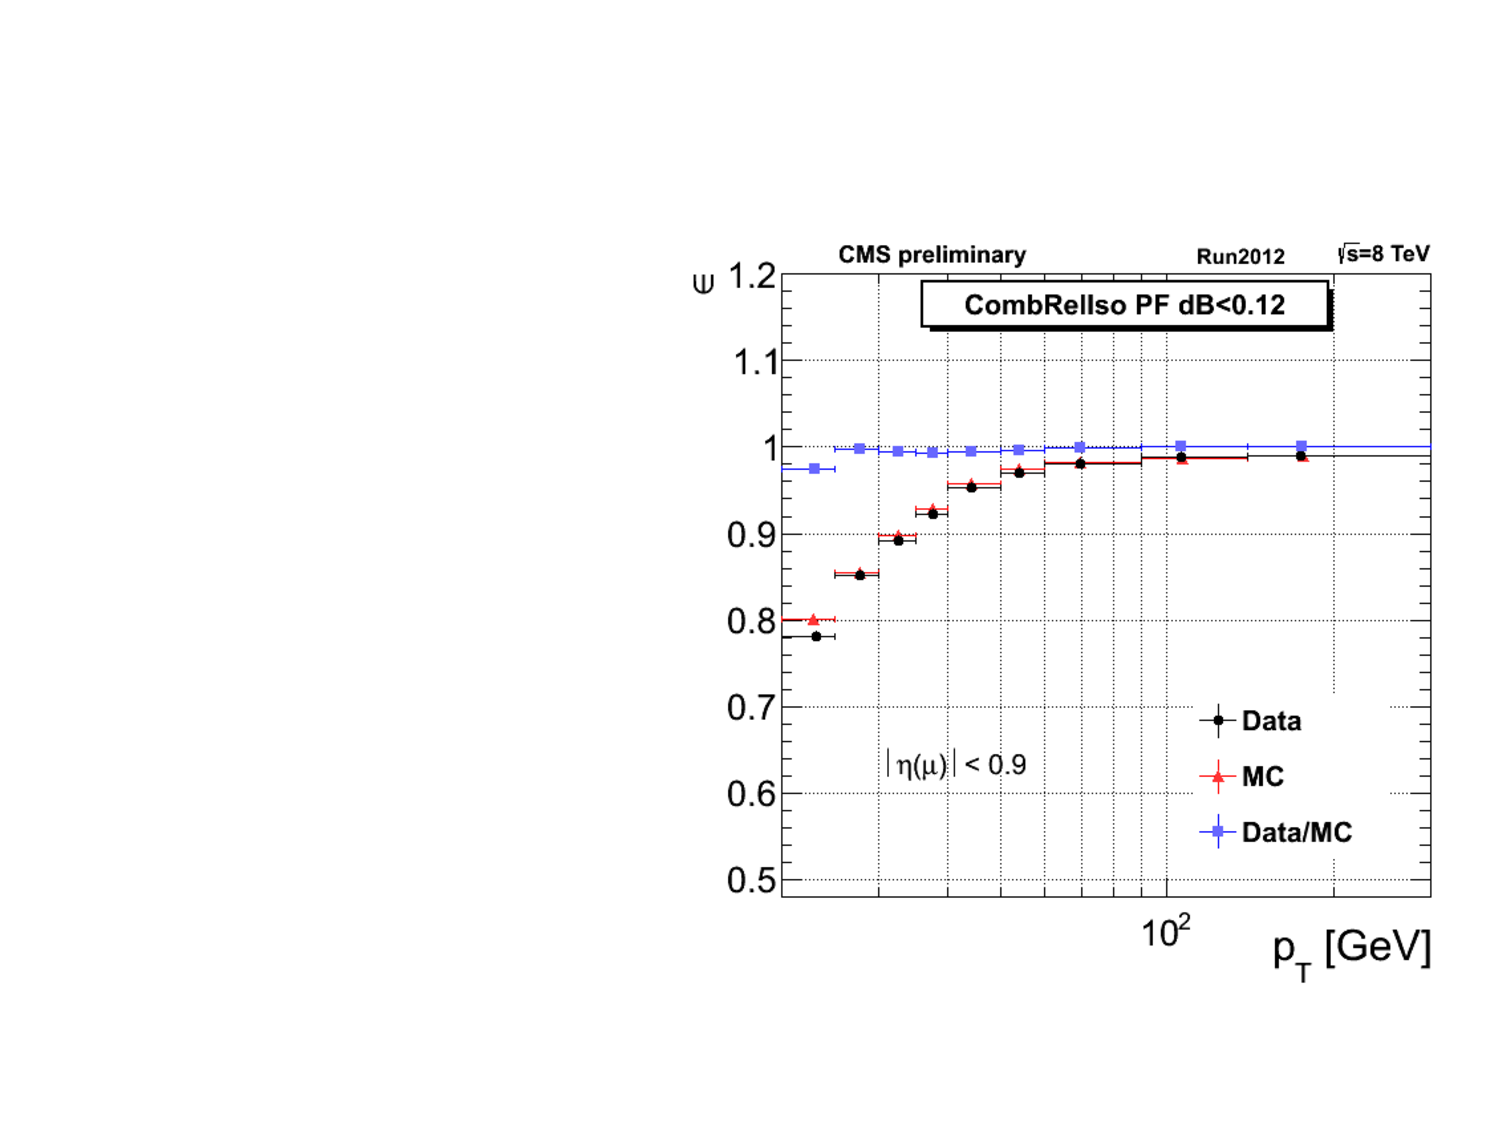
\includegraphics[width=0.49\textwidth]{Figures/ISO_eff.pdf}
		%\rule{35em}{0.5pt}
	\caption[Muon identification and isolation efficiencies using \textit{tag and probe} method.]{Muon identification (\textit{left}) and isolation (\textit{right}) efficiencies determined using \textit{tag and probe} method as a function of a probe $p_T$, for barrel part of the detector$(|\eta|<0.9)$ [NEKA REFERENCA].}
	\label{fig:eff_IDISO}
\end{figure}

\begin{figure}[htbp]
	\centering
		\includegraphics[width=0.5\textwidth]{Figures/trig_eff.pdf}
		%\rule{35em}{0.5pt}
	\caption[Muon trigger efficiency using \textit{tag and probe} method.]{Efficiency for HLT muon trigger for barrel part of the detector $(|\eta|<0.9)$ determined using \textit{tag and probe} method .}
	\label{fig:eff_trig}
\end{figure}  

%-----------------------------------
%	SECTION 3
%-----------------------------------

\subsection{\textit{b-tagging} scale factors}
\label{sec:btag}

CMS simulations describe very well the detector performance, however, it is difficult to accurately model all parameters used in b-tagging algorithms. Procedure used to identify b-jets is described in \ref{sec:btagging} and it depends on track reconstruction efficiency, tracking resolution and other tracking related parameters. Efficiency and missidentification probability are functions of transverse momentum and pseudorapidity of a jet. Therefore, it is very important to determine the b-tagging efficiency from data. The obtained corrections are applied to simulated events as scale factors which are defined as a ratio between efficiency measured in collisions $\epsilon_b^{data}$ and efficiency from simulated events $\epsilon_b^{MC}$:
\begin{equation}
SF_b=\frac{\epsilon_B^{data}}{\epsilon_b^{MC}}
\end{equation}
Scale factor determination has to be performed using b-jet enriched sample such as $t\bar{t}$ or multijets events with jet containing a muon within a $\Delta R <0.4$ cone from the jet axis. The choice of the jet which contains muon relies on the fact that B hadron semileptonic branching ratio is much higher than that for other hadrons ($\sim$ 20$\%$ when including c$\rightarrow$ decays) and such jets are much more likely to arise from B hadron decay. With very high muon detection efficiency at CMS, it is relatively easy to obtain a clean sample with jets containing nonisolated muons. Other efficiency measurement is performed using $t\bar{t}$ enriched sample \cite{CMS:2013vea}.
%by cutting on number of selected jets and isolated leptons in the event and approximating that the $t$ quark decays to $W+b$ exclusively. 
By combining the results from both measurements, scale factors were obtained as a function of jet $p_T$ together with statistical and systematic error for each $p_T$ bin. The same strategy is used to obtain missidentification rates by using the inverted cut on b-tag discriminator. The behavior of both scale factors is approximated by an analytical parametrization as a function of jet $p_T$.  
The usage of the scale factors depends on the number of b-tagged jets in the event. In this analysis two b-tagged jets are required and weight for each event is derived as:
\begin{equation}
w(2|2)=SF_{b||light}(\mathrm{1st\ jet})\times SF_{b||light}(\mathrm{second\ jet})
\end{equation}
where $w(2|2)$ is event weight with 2 jets where both jets are b-tagged. The choice between $SF_{b}$ and $SF_{light}$ depends on the flavor of the jet in the simulation. A jet is considered a b jet if there is a B hadron present among the jet constituents within a cone of 0.4 from the jet axis.    

\begin{figure}
\centering
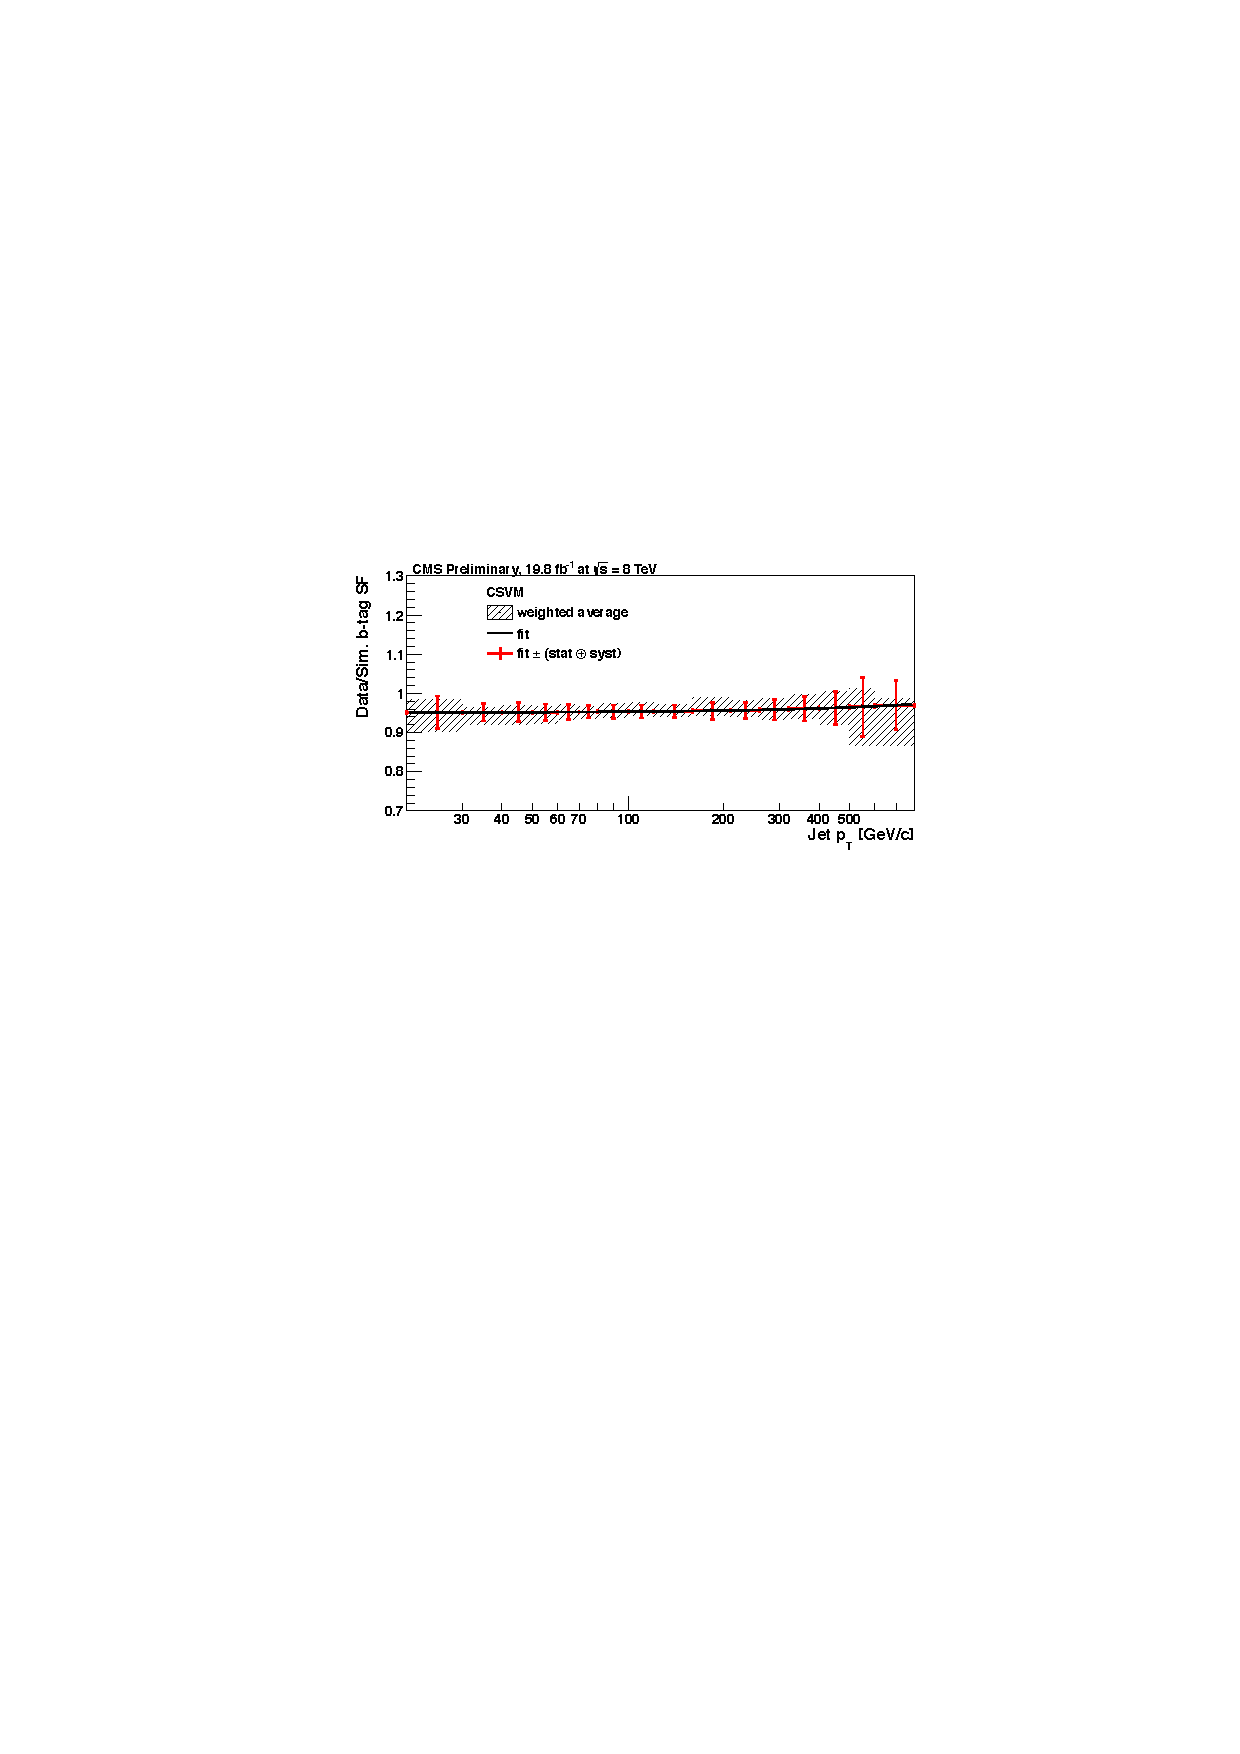
\includegraphics[width=0.6\textwidth]{Figures/b-tagSF.pdf}
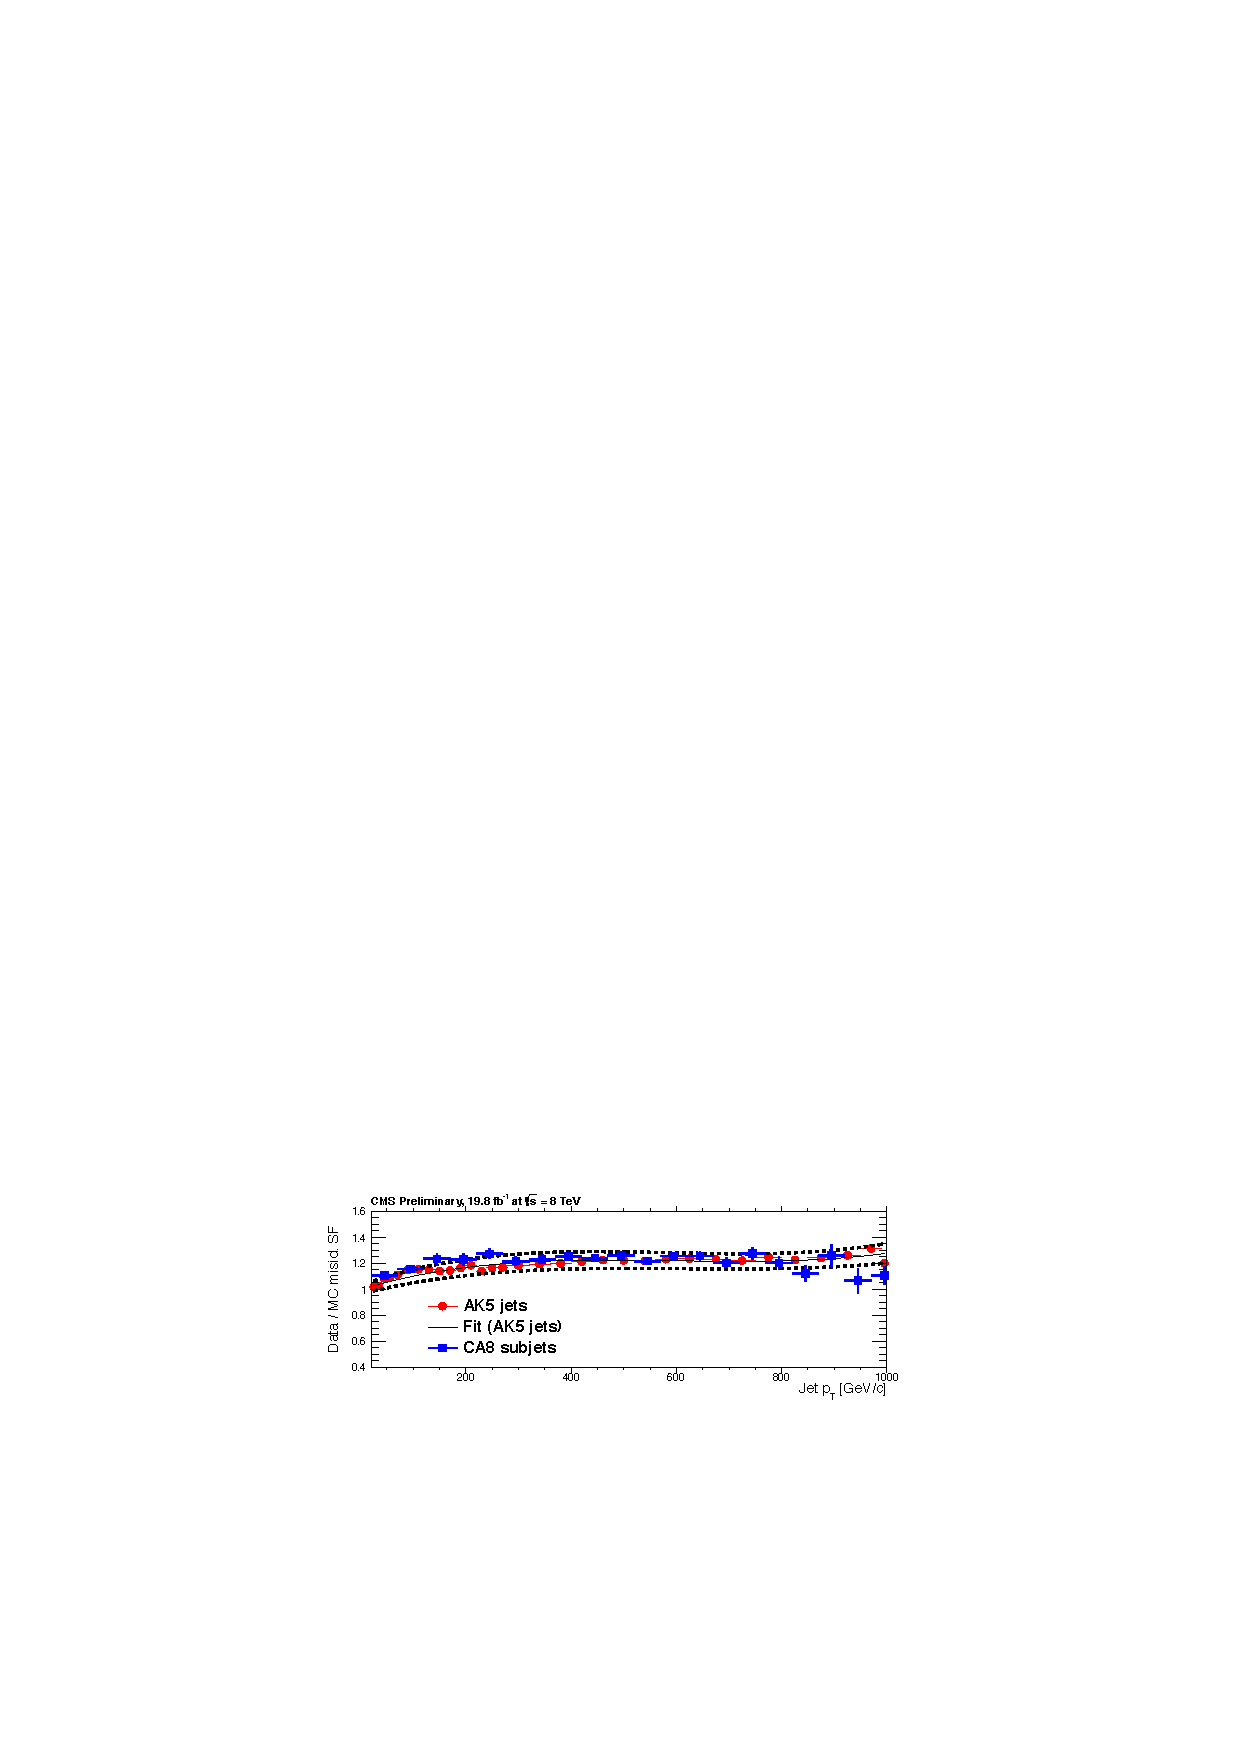
\includegraphics[width=0.6\textwidth]{Figures/miss-tag.pdf}
\label{fig:bSF}
\caption{B-tagging (\textit{up}) and misstag (\textit{bottom}) scale factors. \cite{CMS:2013vea}}
\end{figure}


\section{Event selection}
\label{sec:selection}
Signal events are characterized by presence of a W boson and two jets which have been tagged as coming from b quarks. 
Candidates for a W boson are identified as isolated muons or electron and significant missing energy. 
Jets are identified as particle flow objects clustered with anti-$k_T$ algorithm with a cone size of $0.5$.
Combined secondary vertex (CSV) algorithm is then used to identify jets arising from fragmentation and hadronization of b-quarks which is explained in \ref{sec:btagging}. Signal events are selected using the following requirements:
\begin{itemize}
\item One muon or electron with $p_T>30$ GeV, within $|\eta|<$ 2.1. which passes the trigger requirement and tight ID criteria described in \ref{sec:muID}, and has $I_{rel}^{PF}<0.12\ (0.10)$ in case of muons (electrons).
\item Exactly two jets with jet $p_T>25$ GeV, within $|\eta|<$ 2.4 passing loose ID criteria from \ref{sec:jetID} with distance between lepton and jet $\Delta R>0.5$. 
\item Events containing jets with $p_T>25$ in high pseudorapidity range $2.4<|\eta|<5$ are rejected.
\item Events containing additional lepton with $p_T>10$ GeV, within $|\eta|<$ 2.1, tight ID and isolation are rejected.
\item Both selected jets are required to pass tight CSV discriminator cut of 0.898.
\end{itemize} 

Several detector level distributions are shown in figure \ref{fig:Wbb_prefit_muon} for the muon channel and in figure \ref{fig:Wbb_prefit_electron} for the electron channel obtained after applying all the correction factors described in section \ref{sec:mcSF}. It is visible there is only around 20$\%$ of the Wbb events in the final selection. Therefore it is essential to understand the contributions from all major backgrounds which is described in the next section. 
\begin{figure}[htbp]
	\centering
		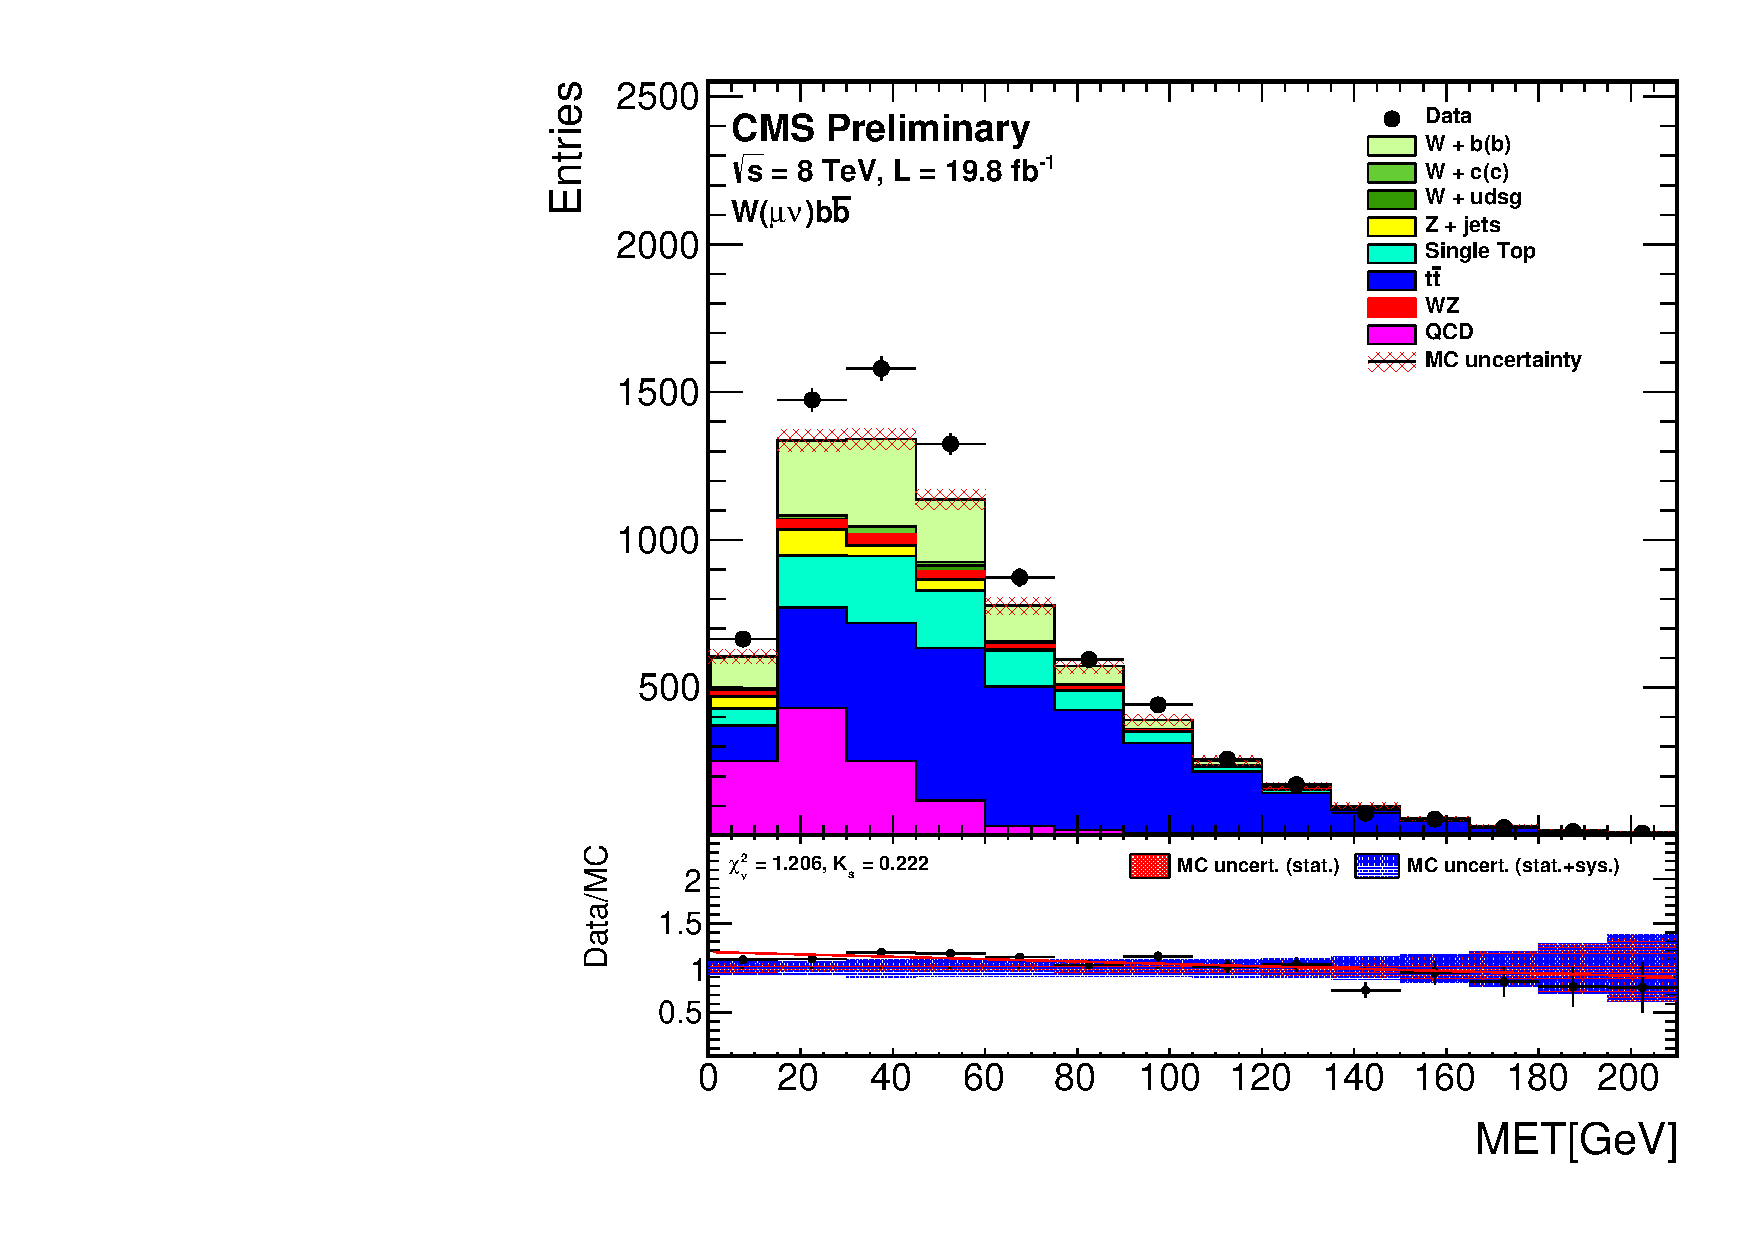
\includegraphics[width=0.48\textwidth]{Figures/Results/Muon/prefit/Wbb_GetMET_doQCD1.pdf}
		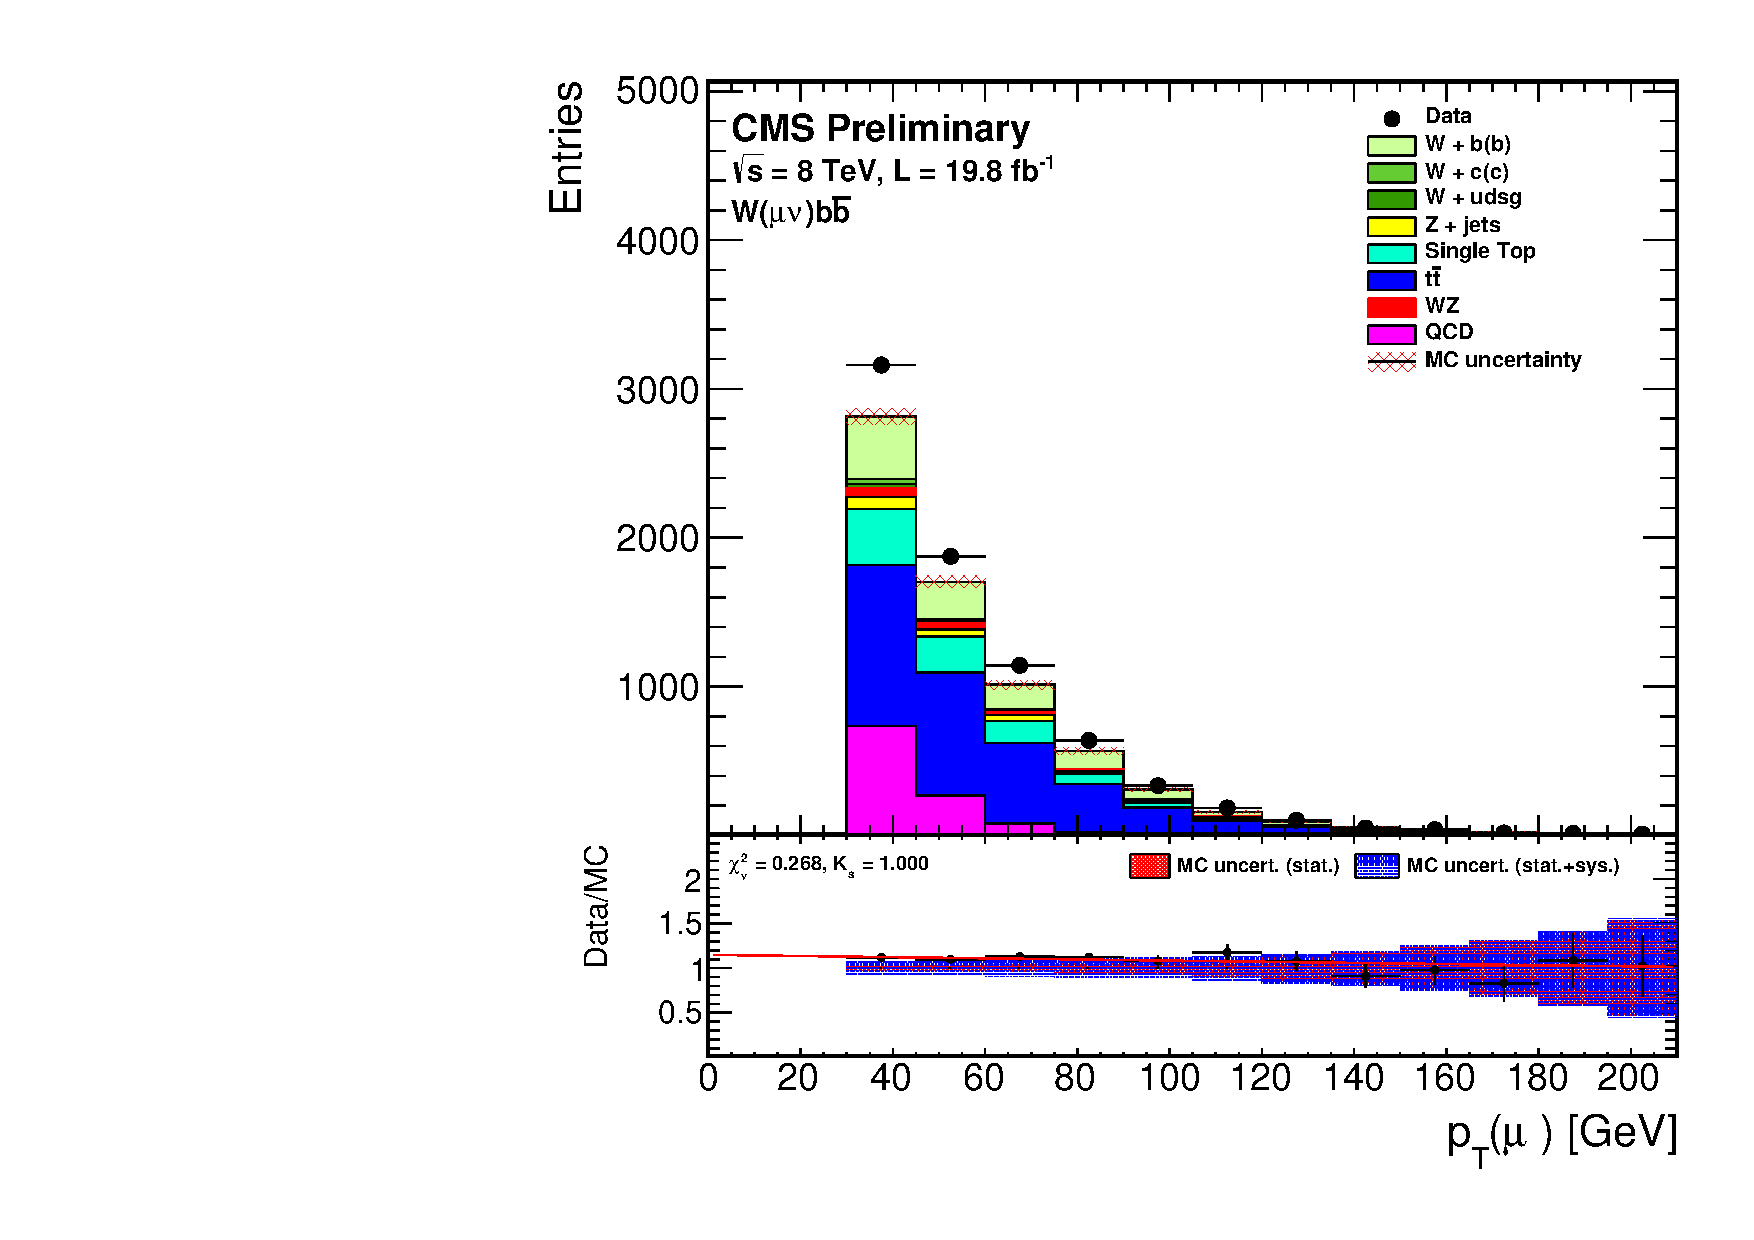
\includegraphics[width=0.48\textwidth]{Figures/Results/Muon/prefit/Wbb_vLepton_pt_doQCD1.pdf}
		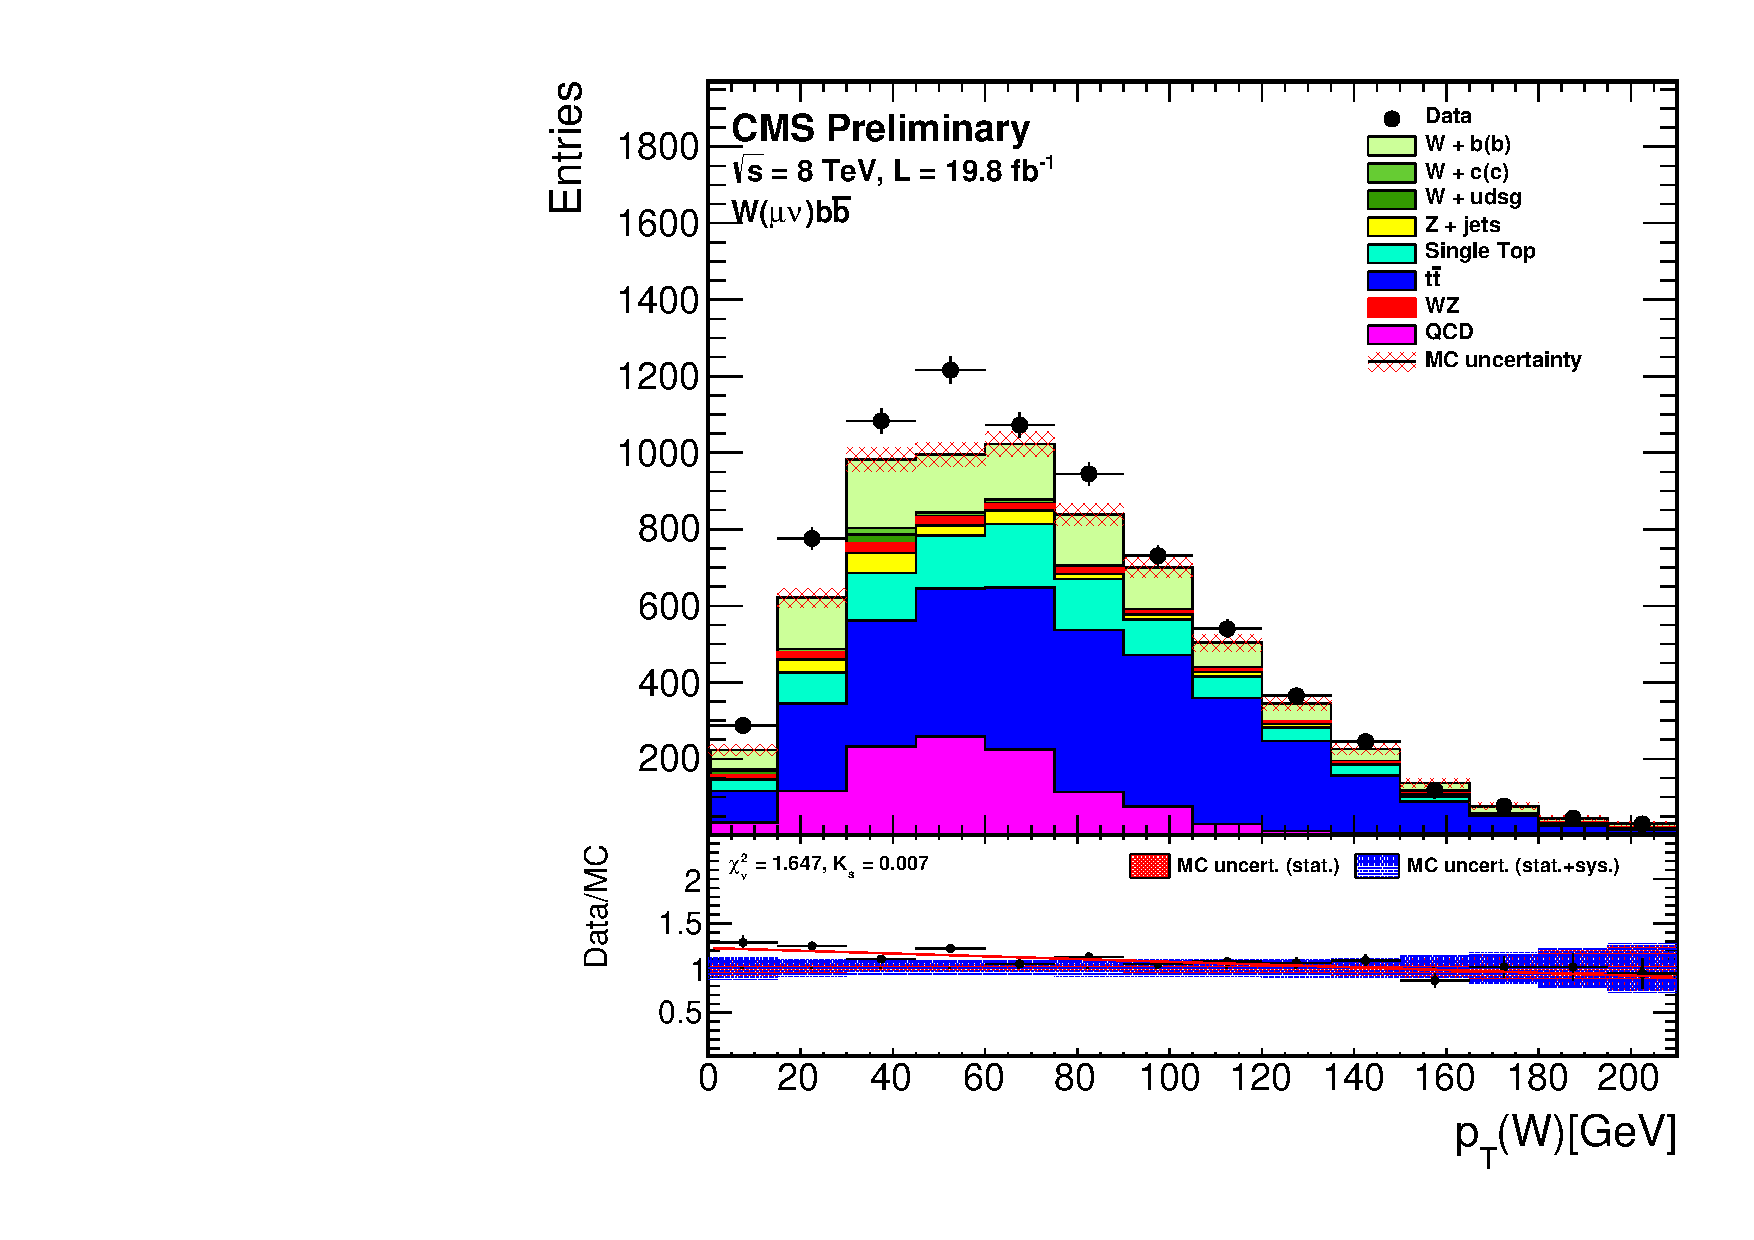
\includegraphics[width=0.48\textwidth]{Figures/Results/Muon/prefit/Wbb_GetWpt_doQCD1.pdf}
		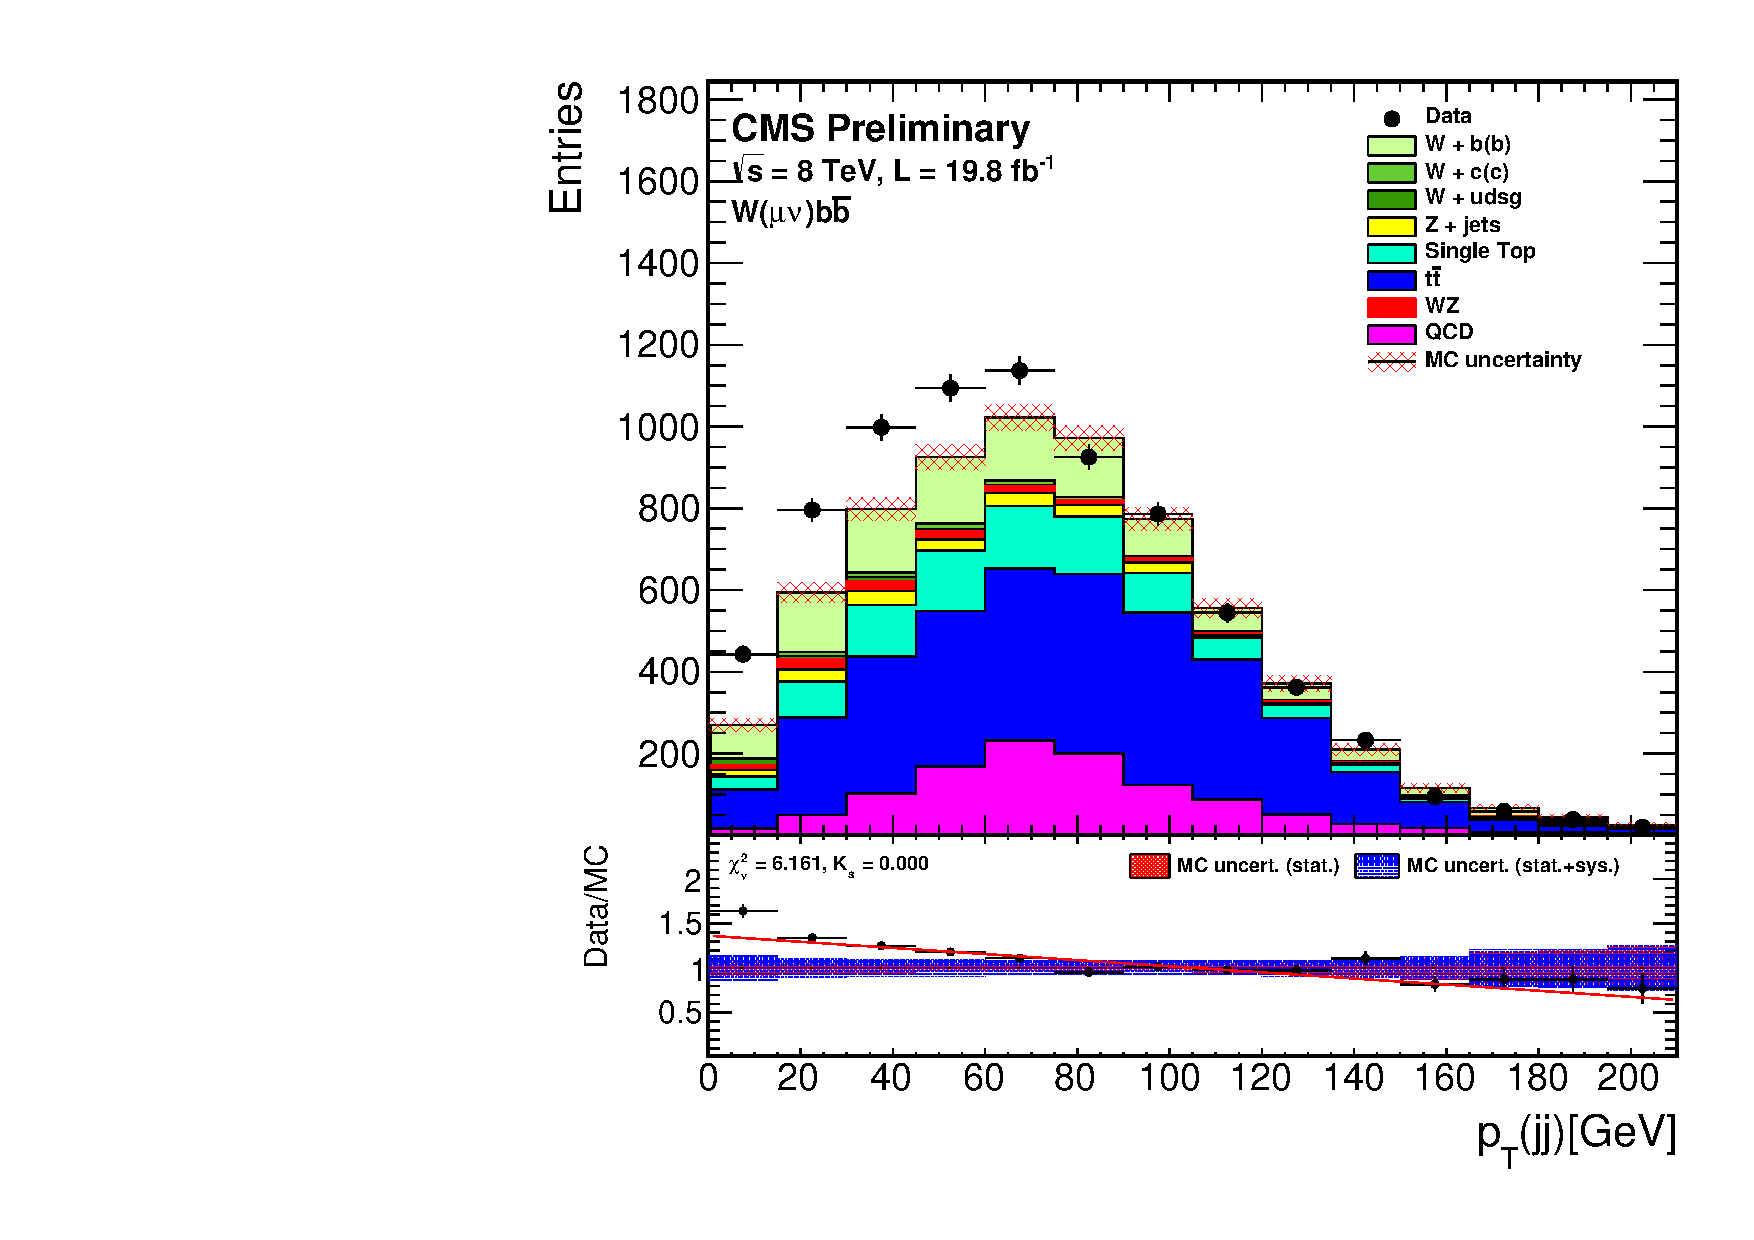
\includegraphics[width=0.48\textwidth]{Figures/Results/Muon/prefit/Wbb_H_pt_doQCD1.pdf}
		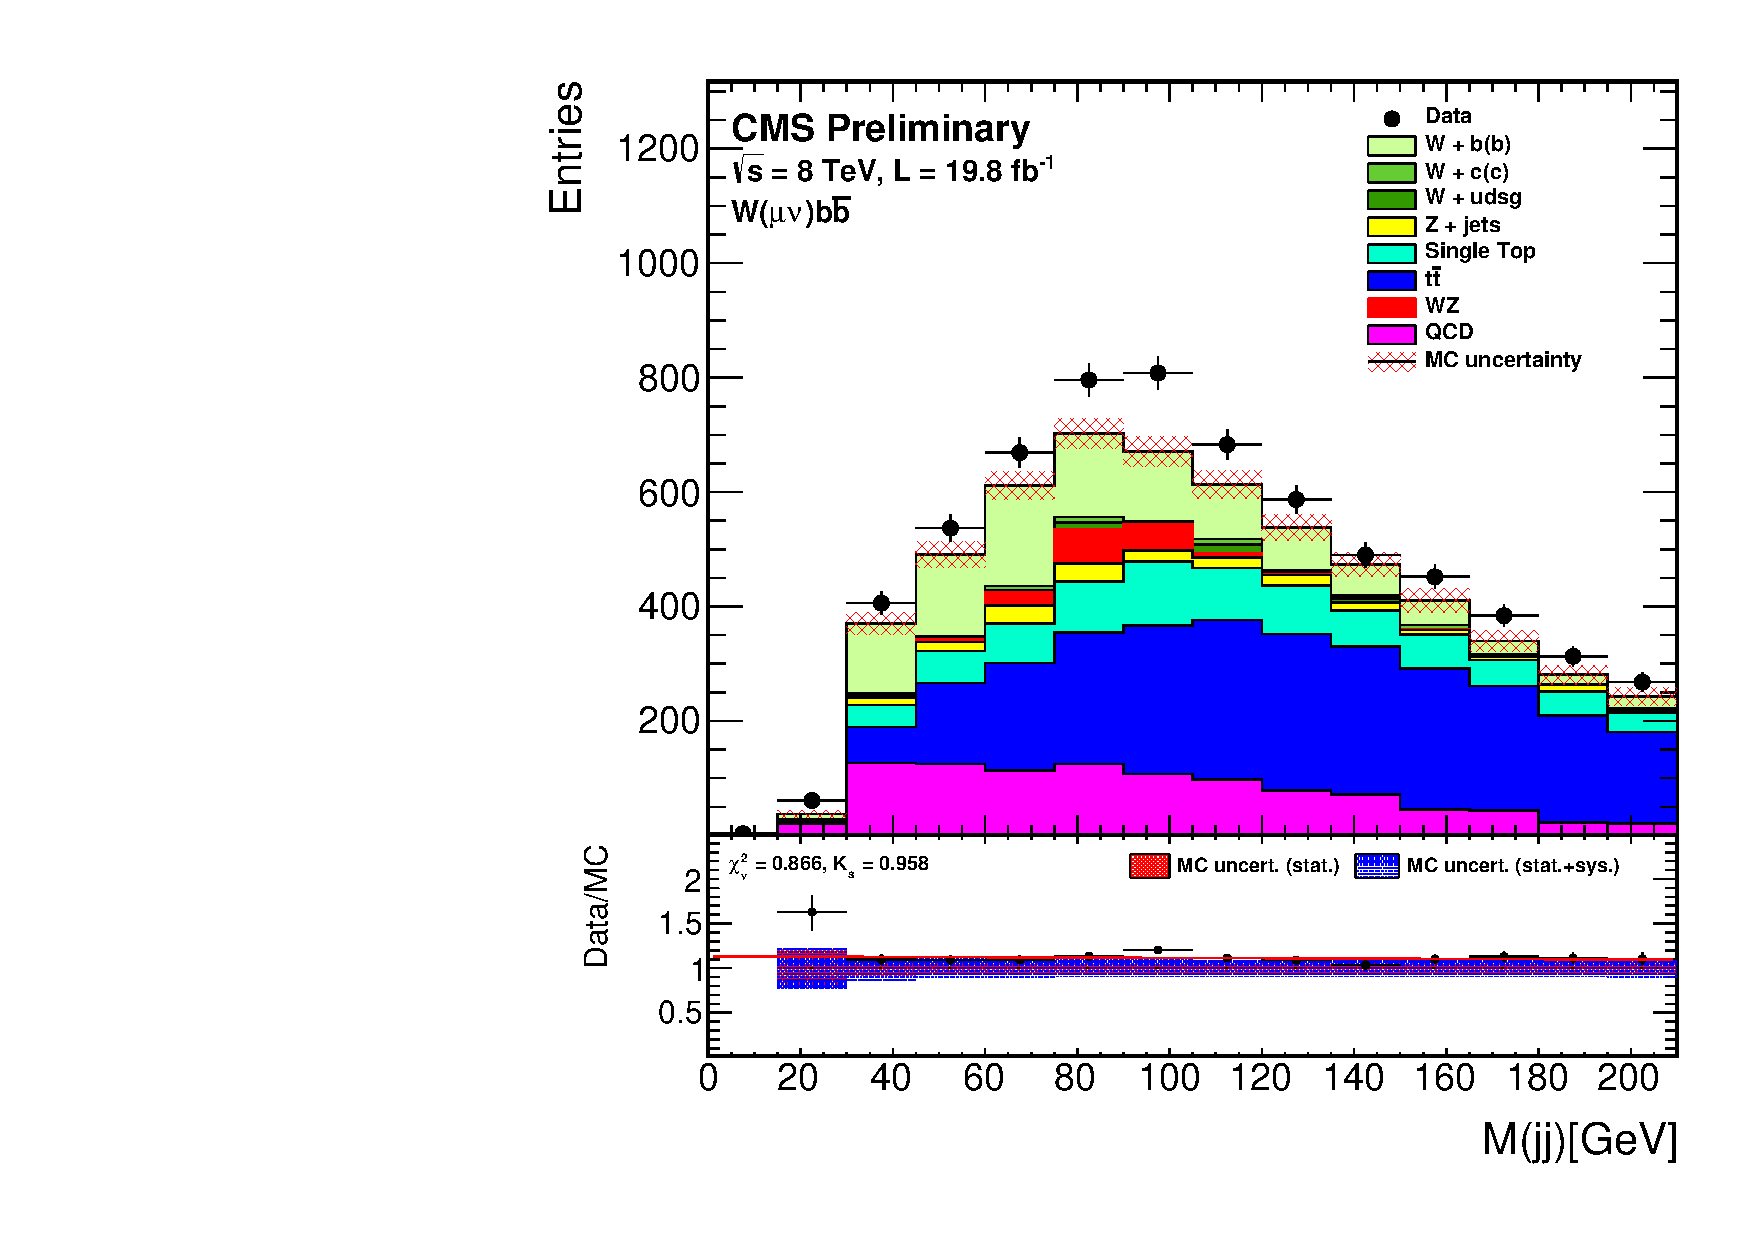
\includegraphics[width=0.48\textwidth]{Figures/Results/Muon/prefit/Wbb_H_mass_doQCD1.pdf}
		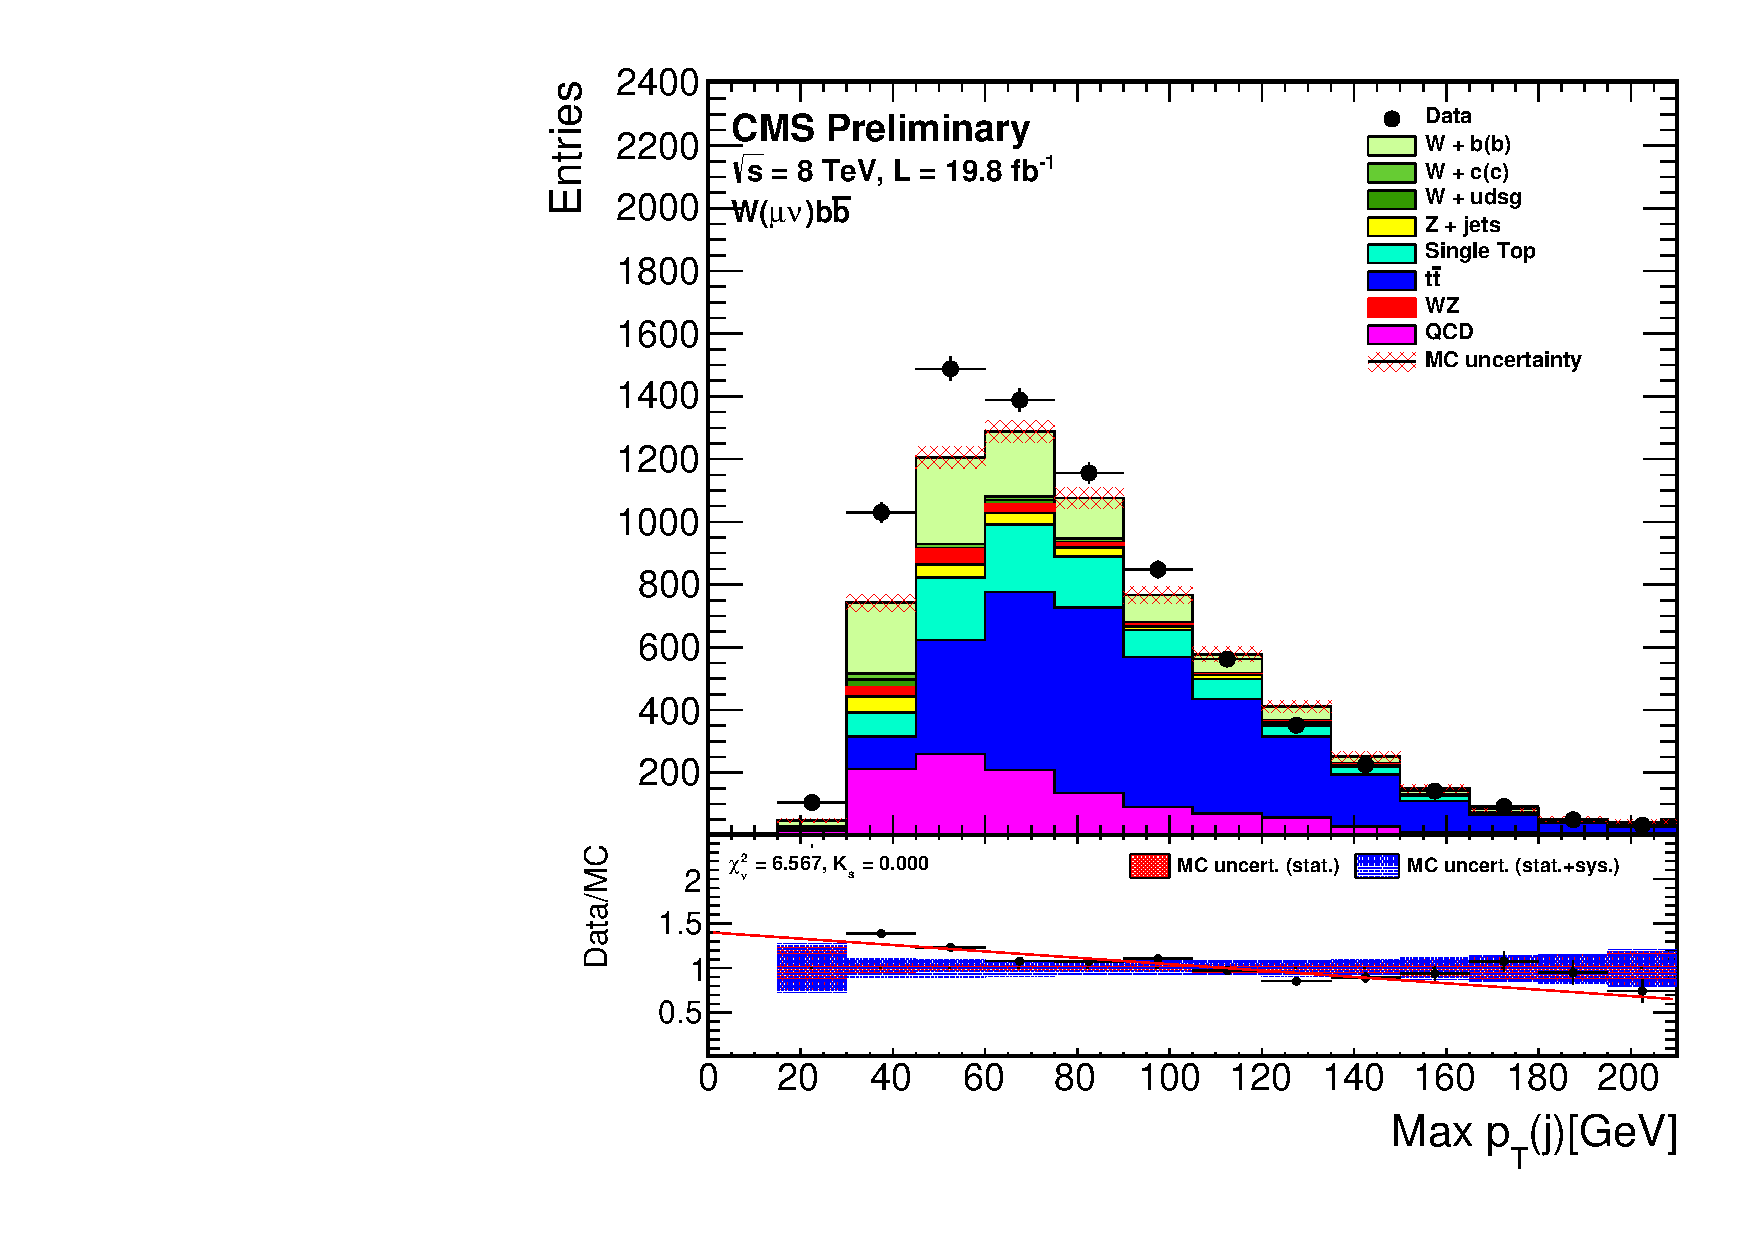
\includegraphics[width=0.48\textwidth]{Figures/Results/Muon/prefit/Wbb_max_hJet_pt_doQCD1.pdf}		
		%\rule{35em}{0.5pt}
	\caption[Signal region detector level distributions for the muon channel]{Various signal region distributions for the electron channel: missing energy, lepton transverse momentum, W transverse momentum, invariant mass and transverse momentum of two b jets and highest jet transverse momentum.}
	\label{fig:Wbb_prefit_muon}
\end{figure}
\begin{figure}[htbp]
	\centering
		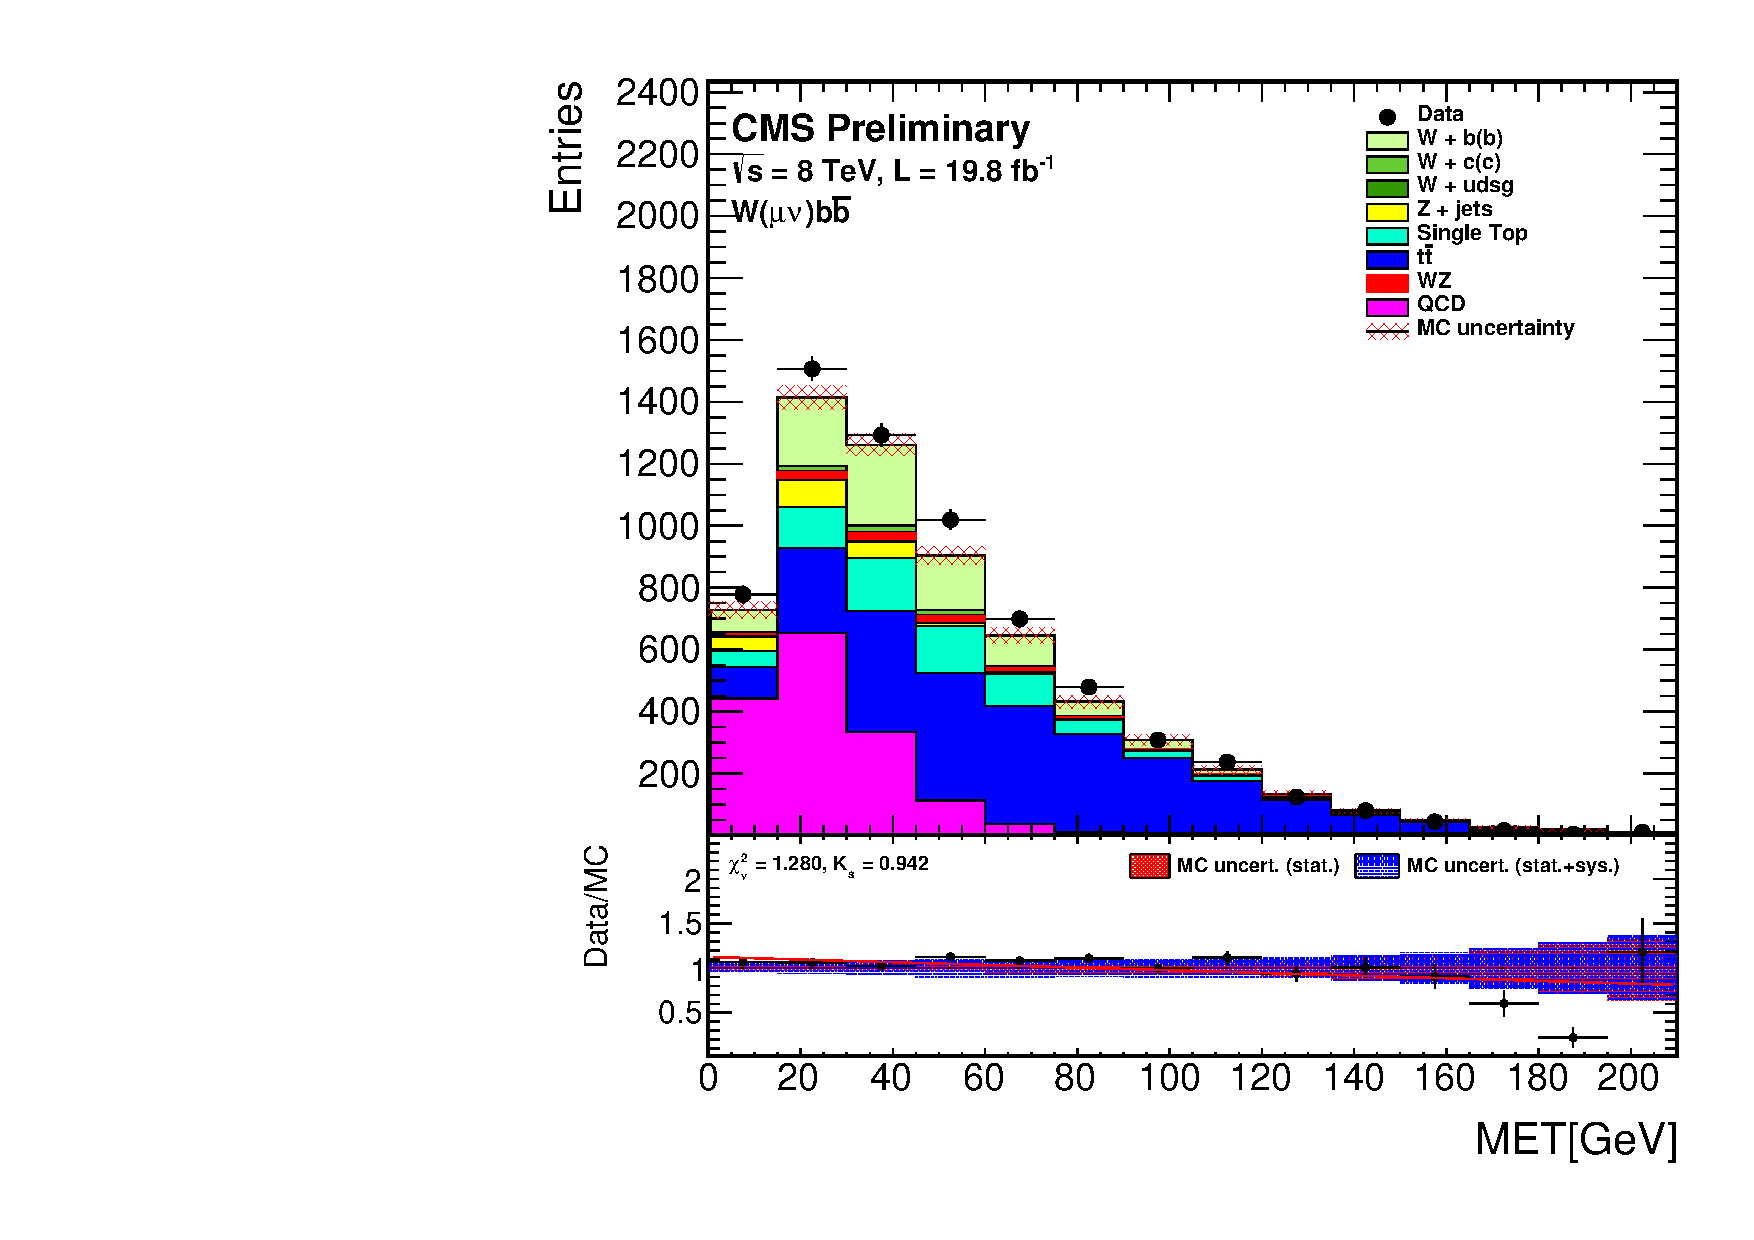
\includegraphics[width=0.48\textwidth]{Figures/Results/Electron/prefit/Wbb_GetMET_doQCD1.pdf}
		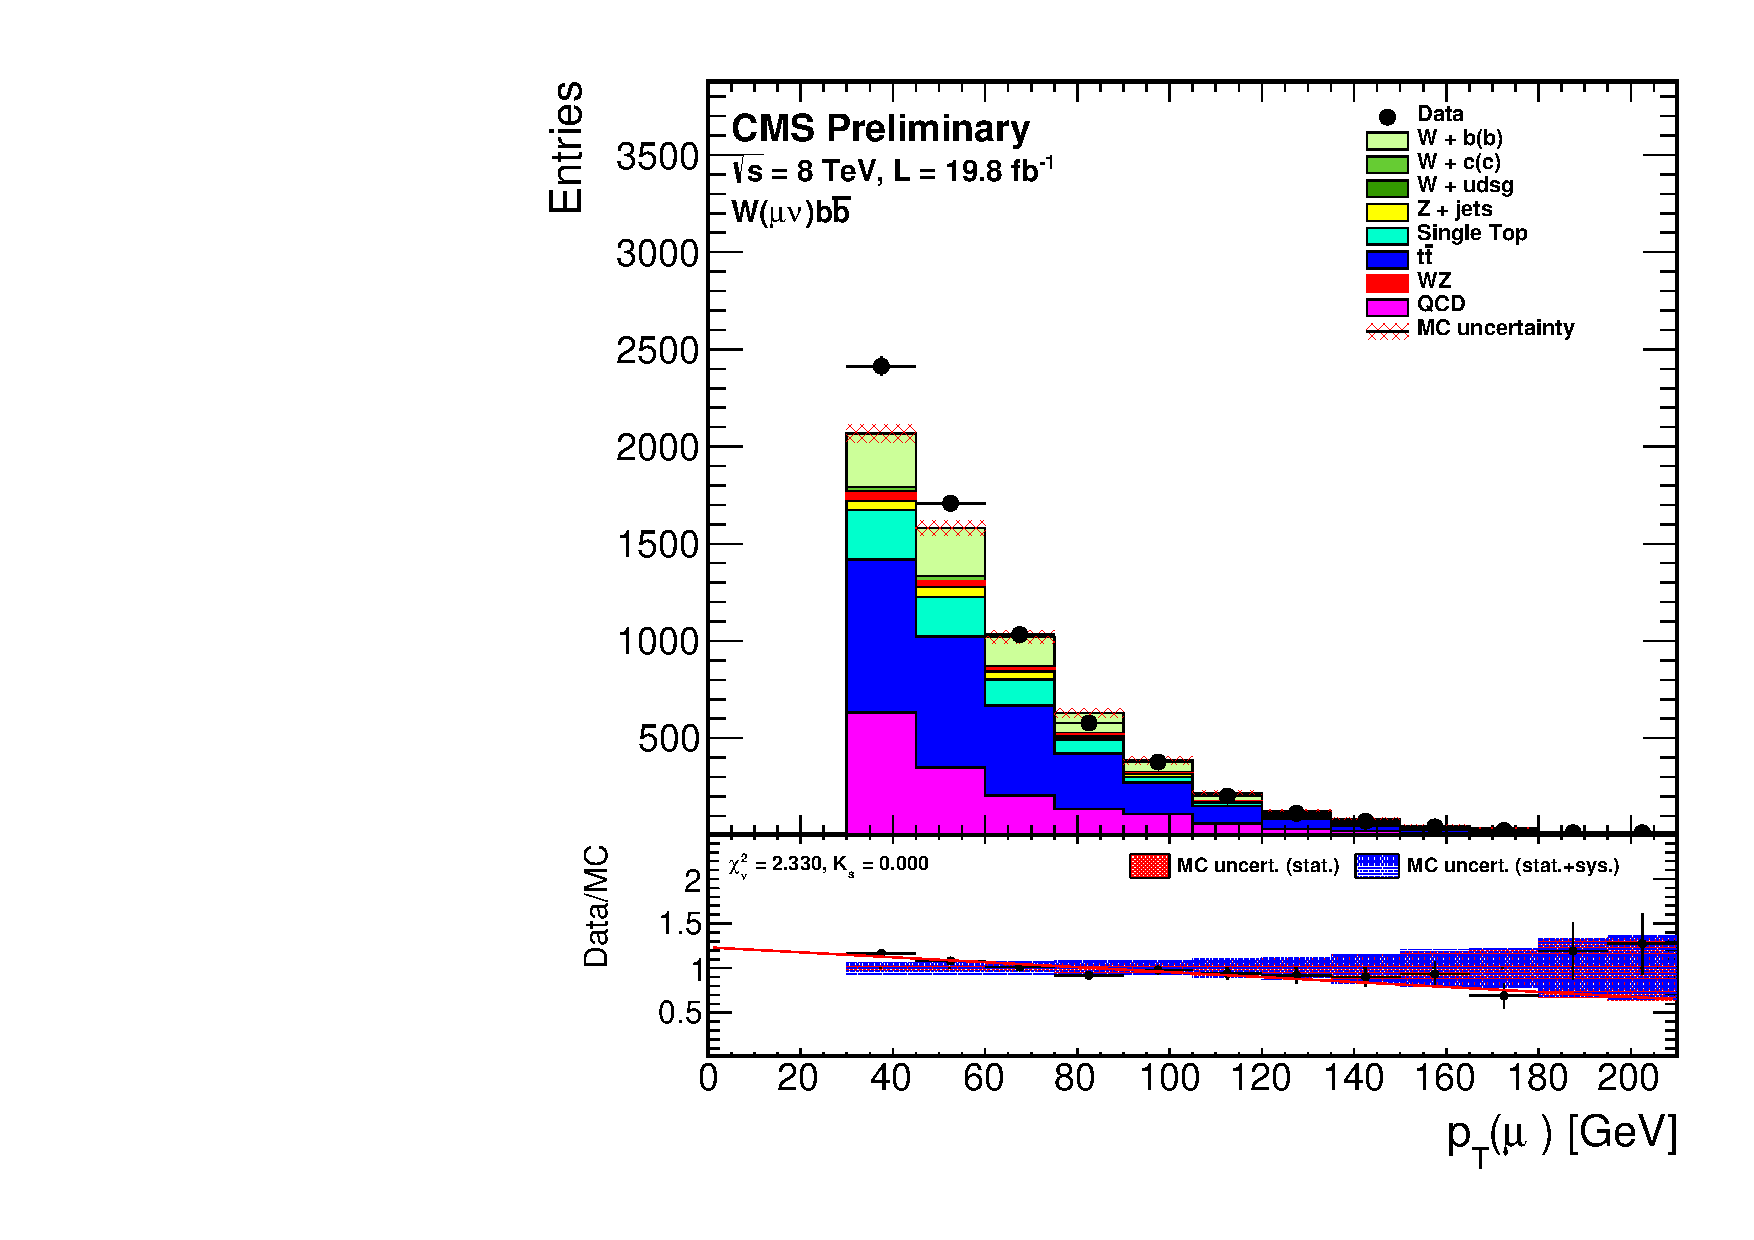
\includegraphics[width=0.48\textwidth]{Figures/Results/Electron/prefit/Wbb_vLepton_pt_doQCD1.pdf}
		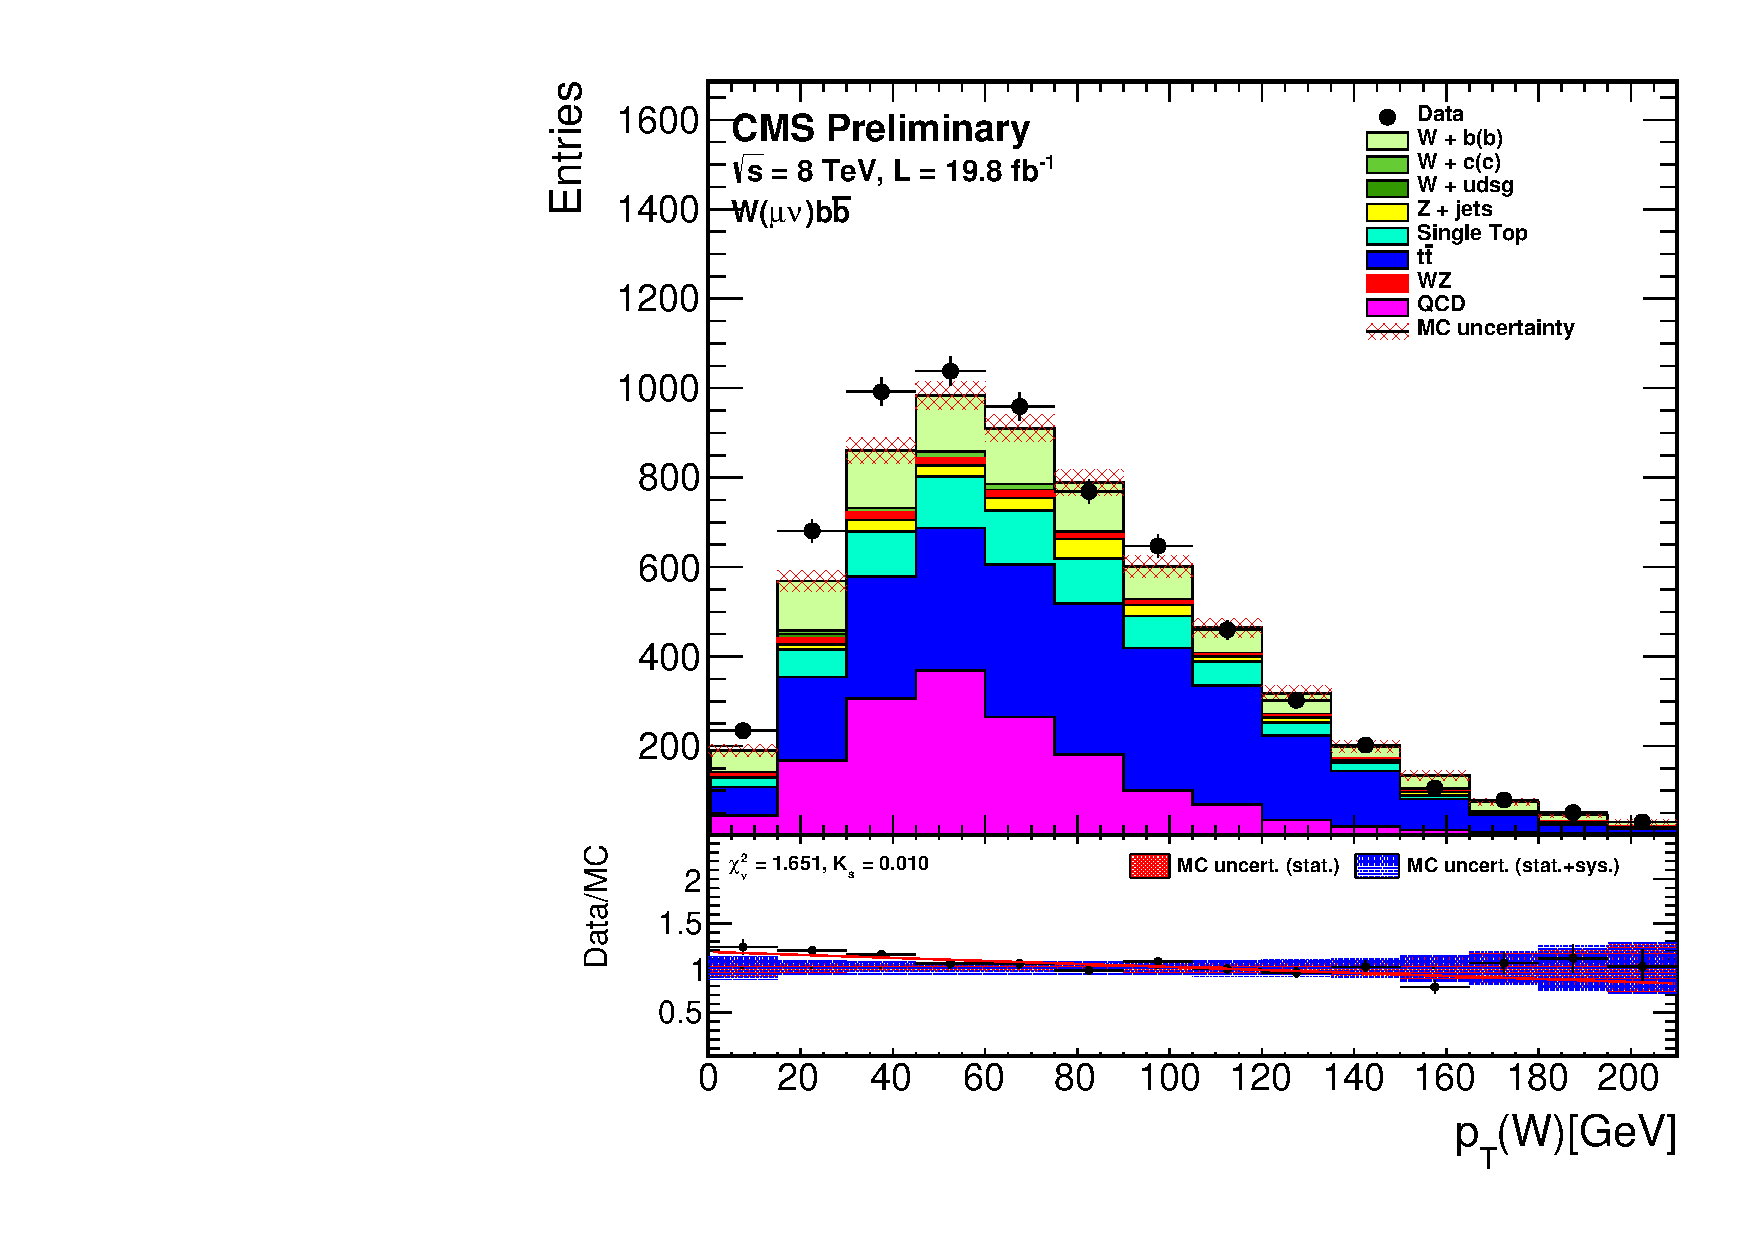
\includegraphics[width=0.48\textwidth]{Figures/Results/Electron/prefit/Wbb_GetWpt_doQCD1.pdf}
		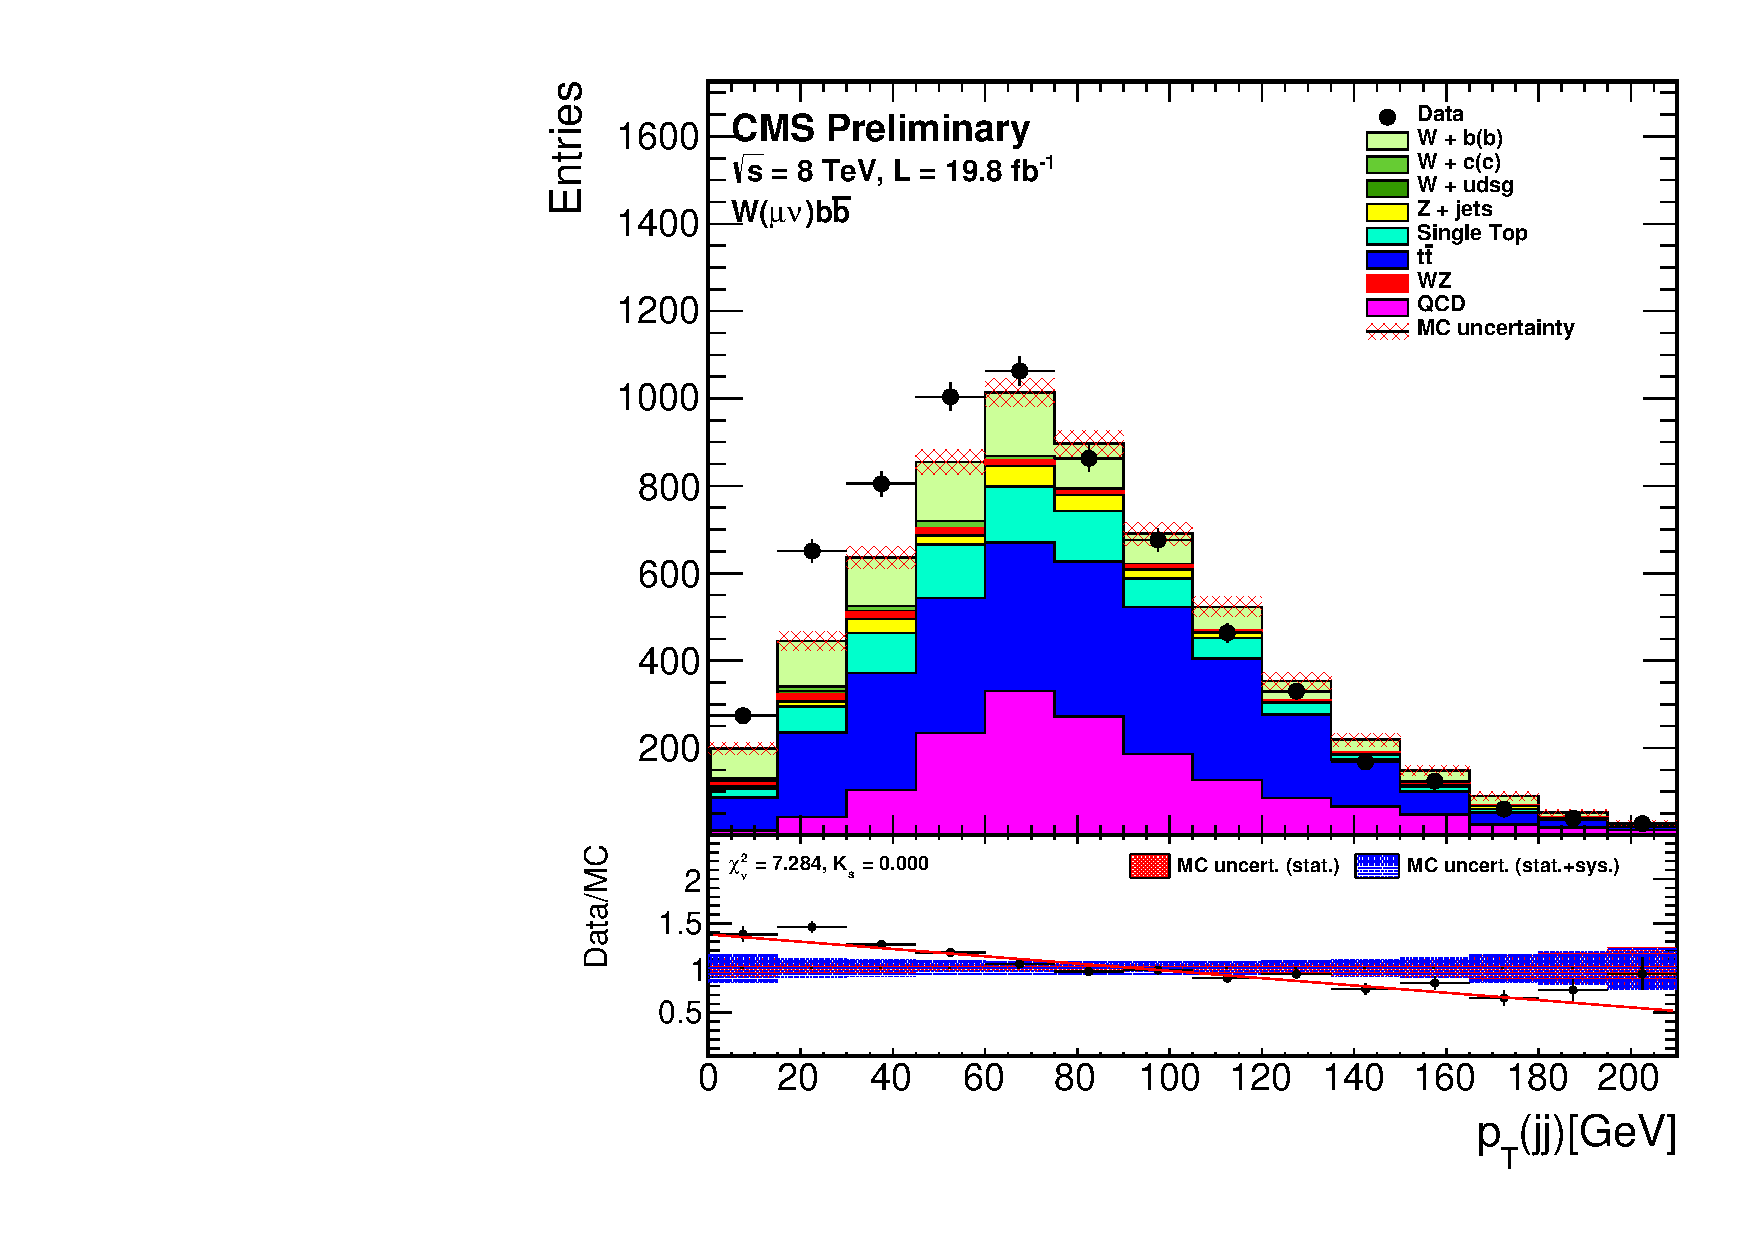
\includegraphics[width=0.48\textwidth]{Figures/Results/Electron/prefit/Wbb_H_pt_doQCD1.pdf}
		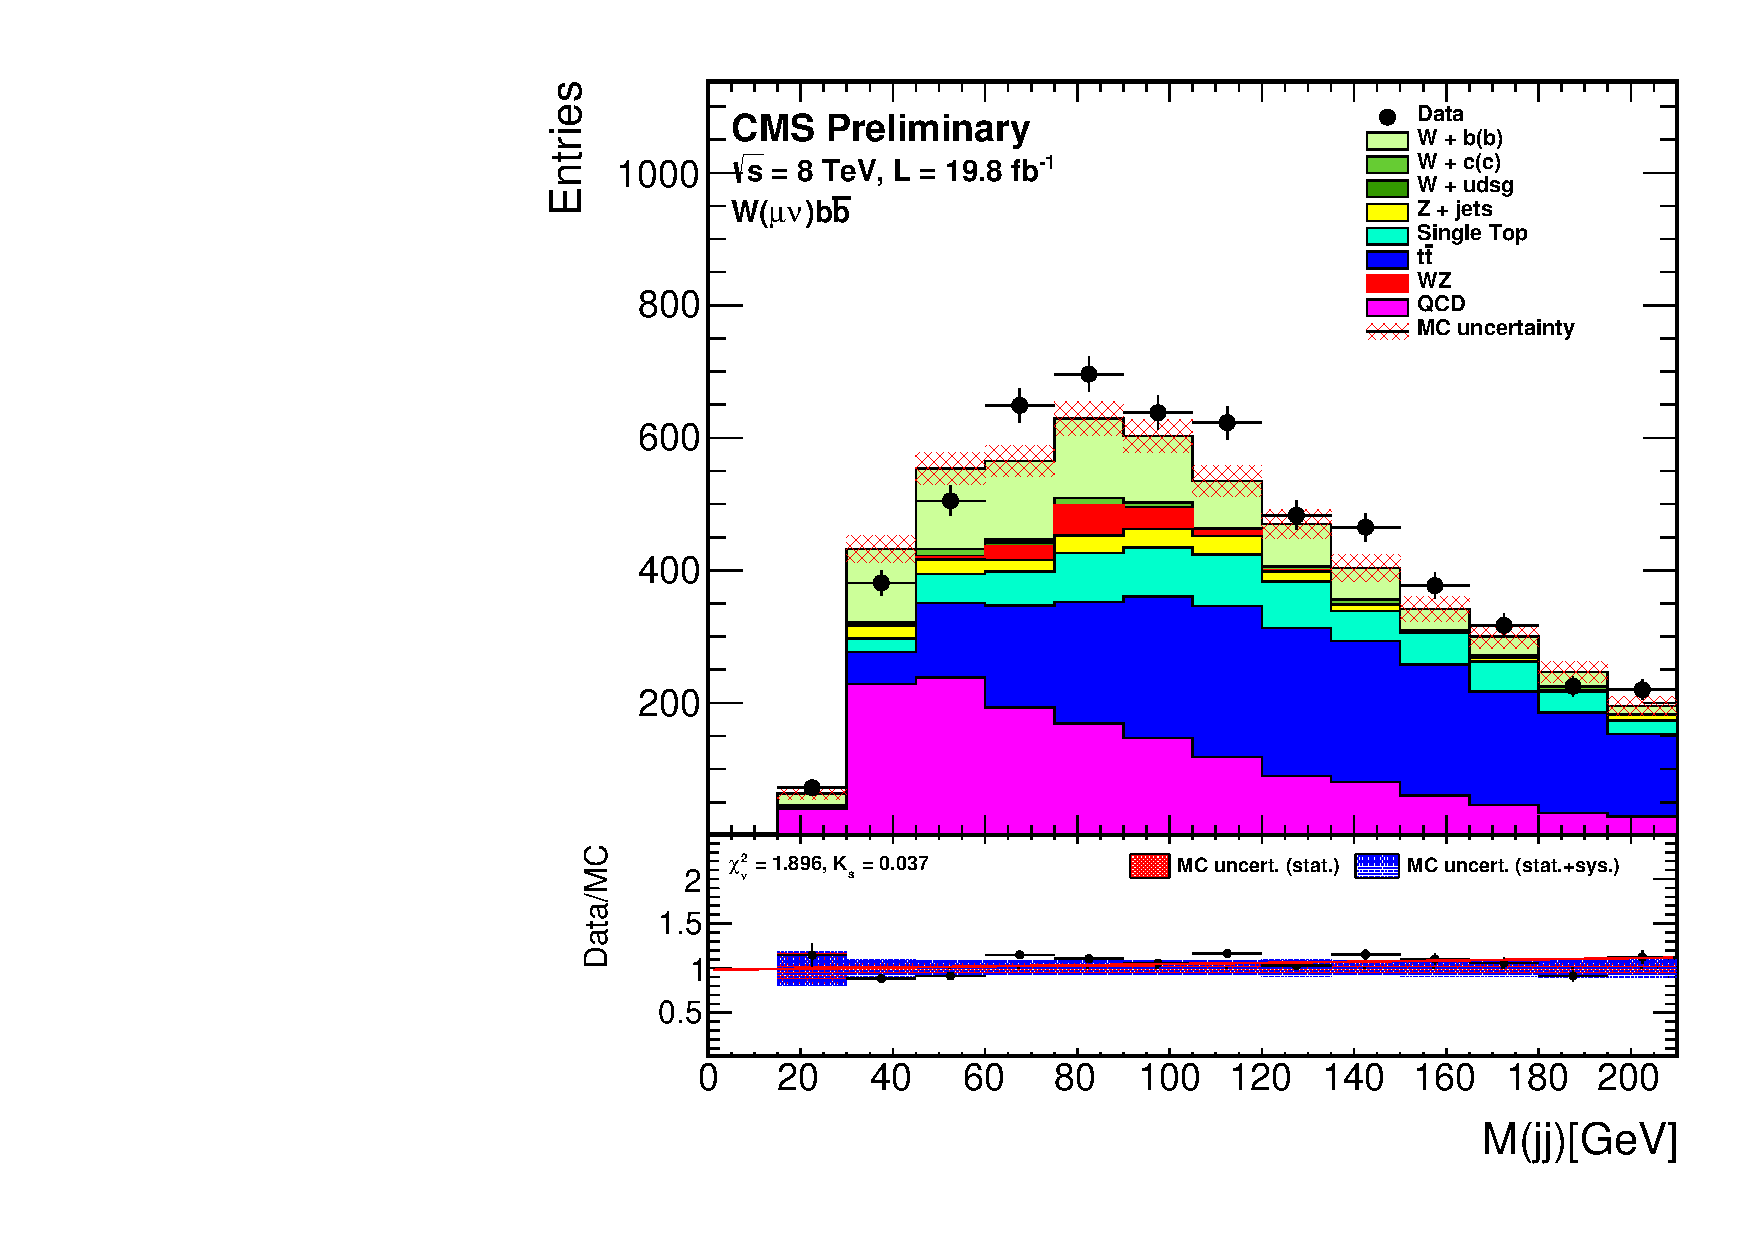
\includegraphics[width=0.48\textwidth]{Figures/Results/Electron/prefit/Wbb_H_mass_doQCD1.pdf}
		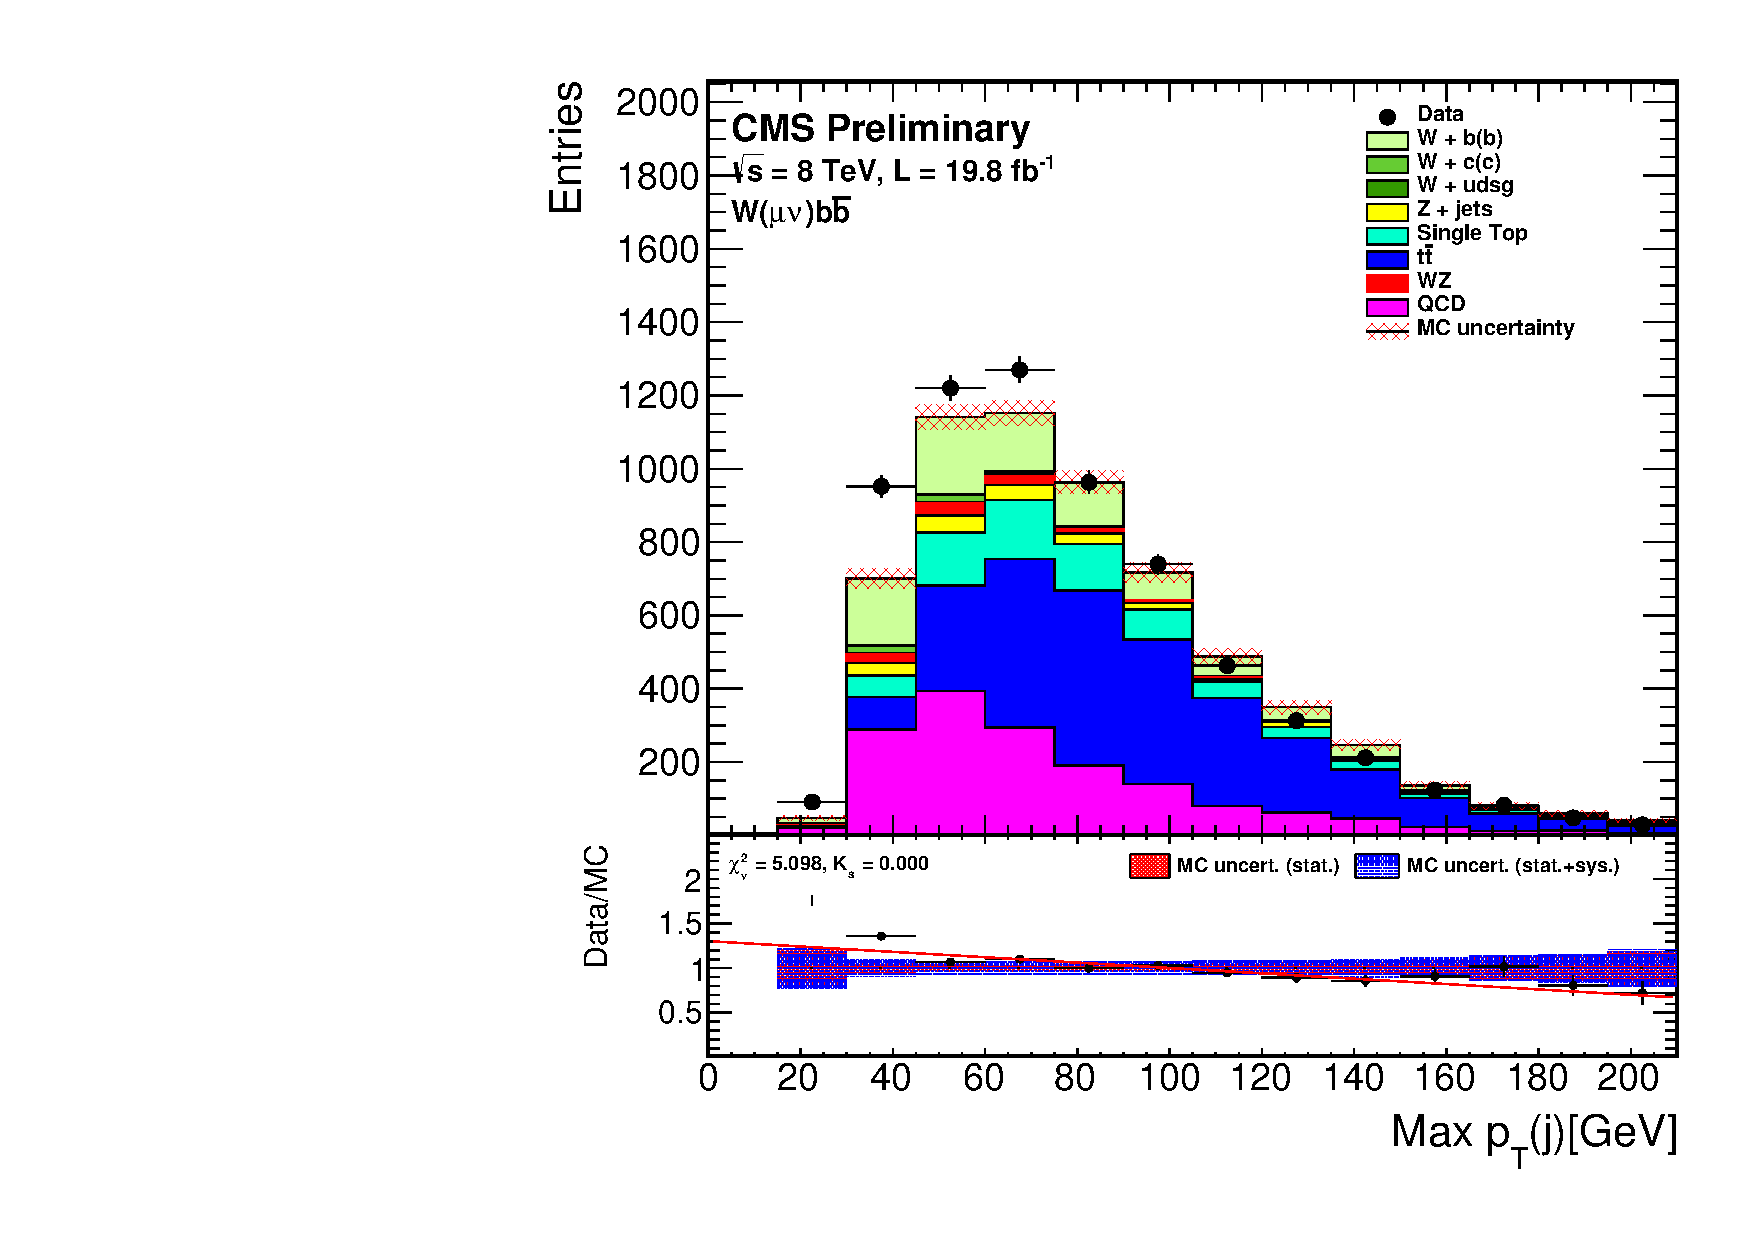
\includegraphics[width=0.48\textwidth]{Figures/Results/Electron/prefit/Wbb_max_hJet_pt_doQCD1.pdf}		
		%\rule{35em}{0.5pt}
	\caption[Signal region distributions for the electron channel]{Various signal region distributions for the electron channel: missing energy, lepton transverse momentum, W transverse momentum, invariant mass and transverse momentum of two b jets and highest jet transverse momentum. }
	\label{fig:Wbb_prefit_electron}
\end{figure}

%----------------------------------------------------------------------------------------
%	SECTION 4
%----------------------------------------------------------------------------------------

\section{Background contribution}
\label{sec:background}
After applying all selection cuts described in the previous section, major backgrounds that remain are top quark, Z+jets, W+jets, diboson and QCD background. Each of the background contributions is described in detail below. 

\begin{figure}[htbp]
	\centering
		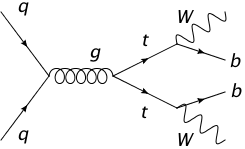
\includegraphics[width=0.37\textwidth]{Figures/FD-tt.png}
		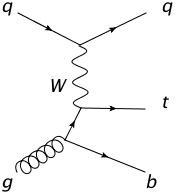
\includegraphics[width=0.245\textwidth]{Figures/FD-st.png}
		\includegraphics[width=0.25\textwidth]{Figures/FD-WJ.png}
	\caption[Feynmann diagrams showing major backgrounds]{Feynmann diagrams for major backgrounds: $t\bar{t}$, single top and W+jets. [DODATI OSTALE DIJAGRAME]}
	\label{fig:backgrounds}
\end{figure}

\subsection{Top quark background}

Production of $t\bar{t}$ pairs and single top represent a challenging background at the LHC because of their relatively large production cross sections. $t\bar{t}$ events are largely reduced by requiring additional jet veto. Single top background is more difficult to reduce using only topological cuts. However, its production cross-section is smaller resulting in a smaller contribution in the final distributions. Nevertheless, the contribution from the top quark backgrounds in the final sample is around 60$\%$.
\par As the $t\bar{t}$ background is large, it is mandatory to perform a test of its normalization. For that purpose, a separate control region is defined requiring additional jet activity. This results in a $t\bar{t}$ enriched sample. Various distributions including missing energy, lepton transverse momentum, W transverse momentum, invariant mass and transverse momentum of two b jets and highest jet transverse momentum are shown in figure \ref{fig:TT_CR}. It is visible that the shape of the distributions is in agreement between data and simulation, but the difference in the overall normalization after applying all scale factors is of the order of 12$\%$. The disagreement is likely coming from the b-tagging scale factors not being properly determined. This is taken into account while performing the global fit performed in order to extract the number of signal events extraction which will be described in detail in the next chapter. 
\begin{figure}[htbp]
	\centering
		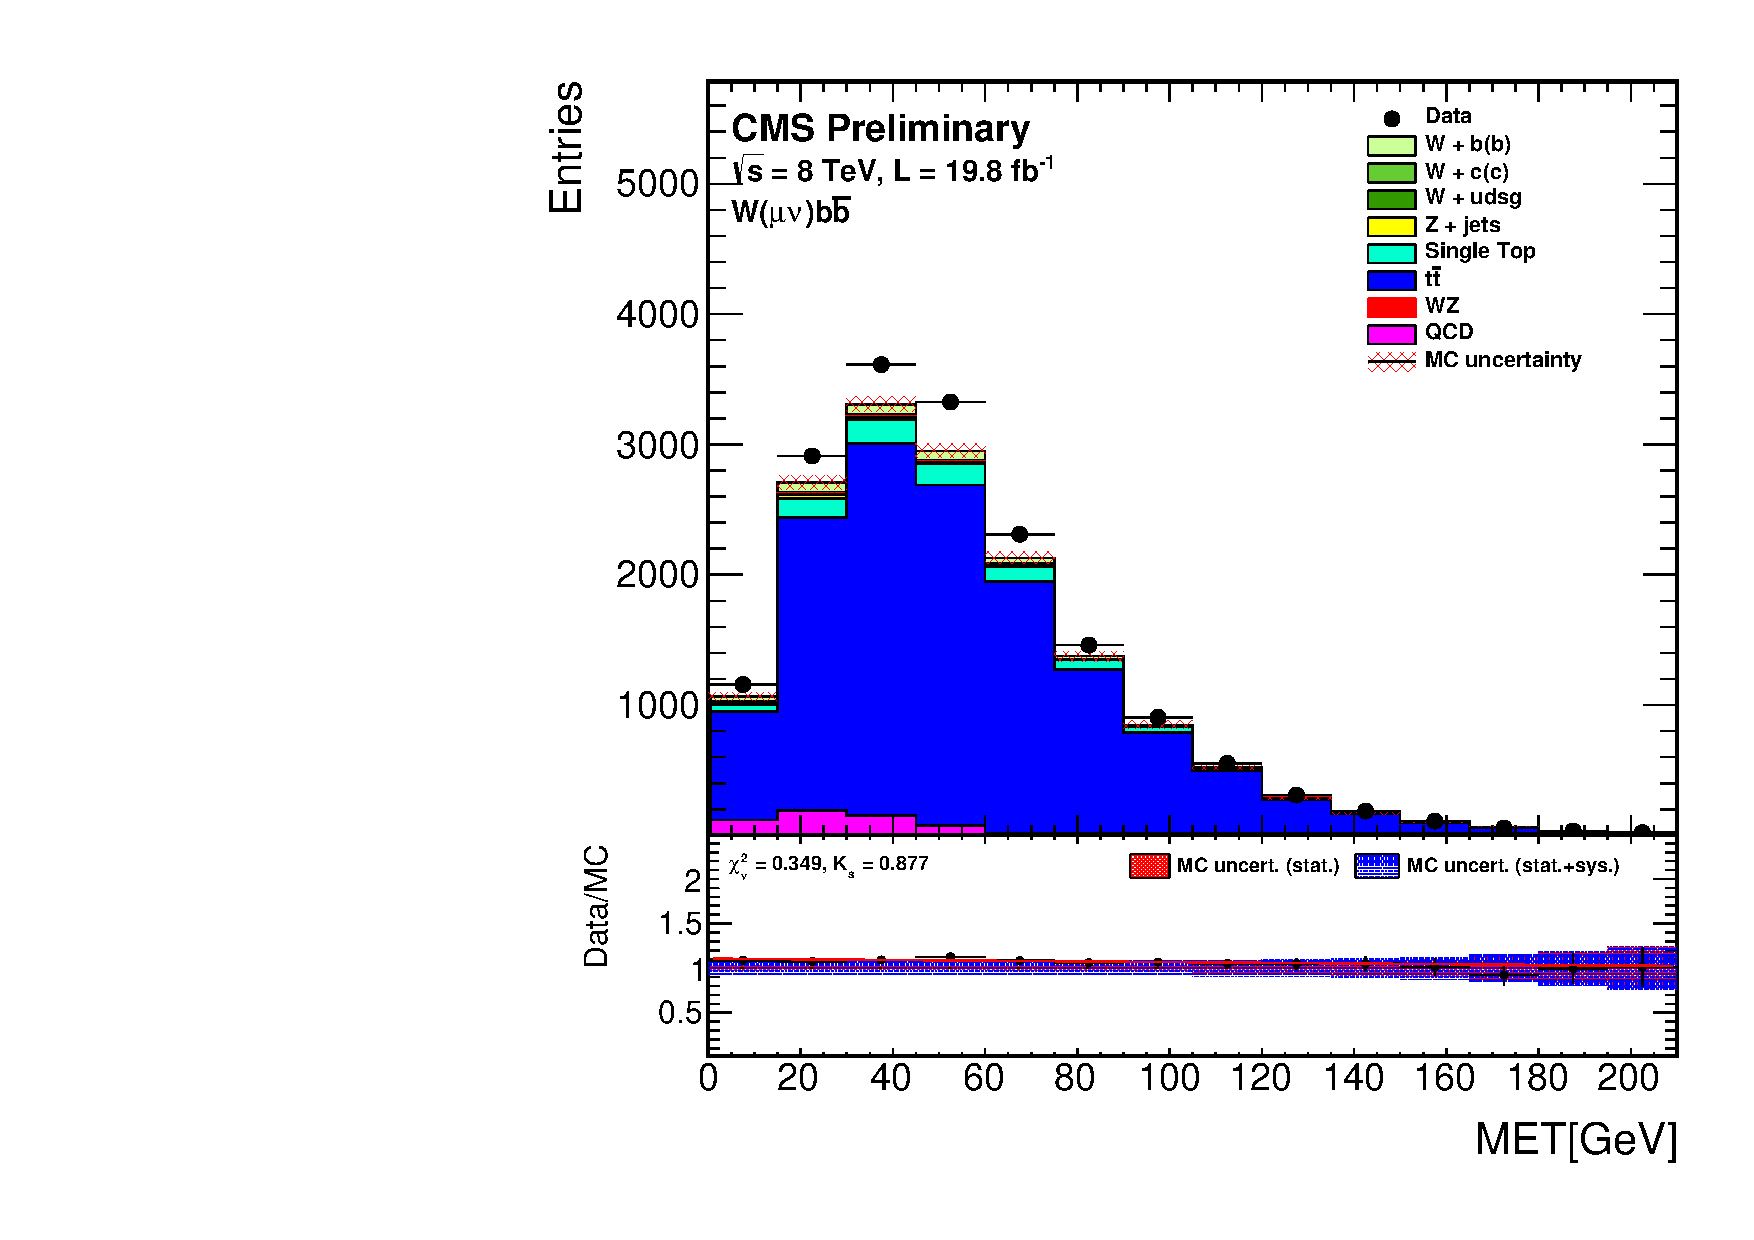
\includegraphics[width=0.48\textwidth]{Figures/Results/Muon/prefit/TT_GetMET_doQCD1.pdf}
		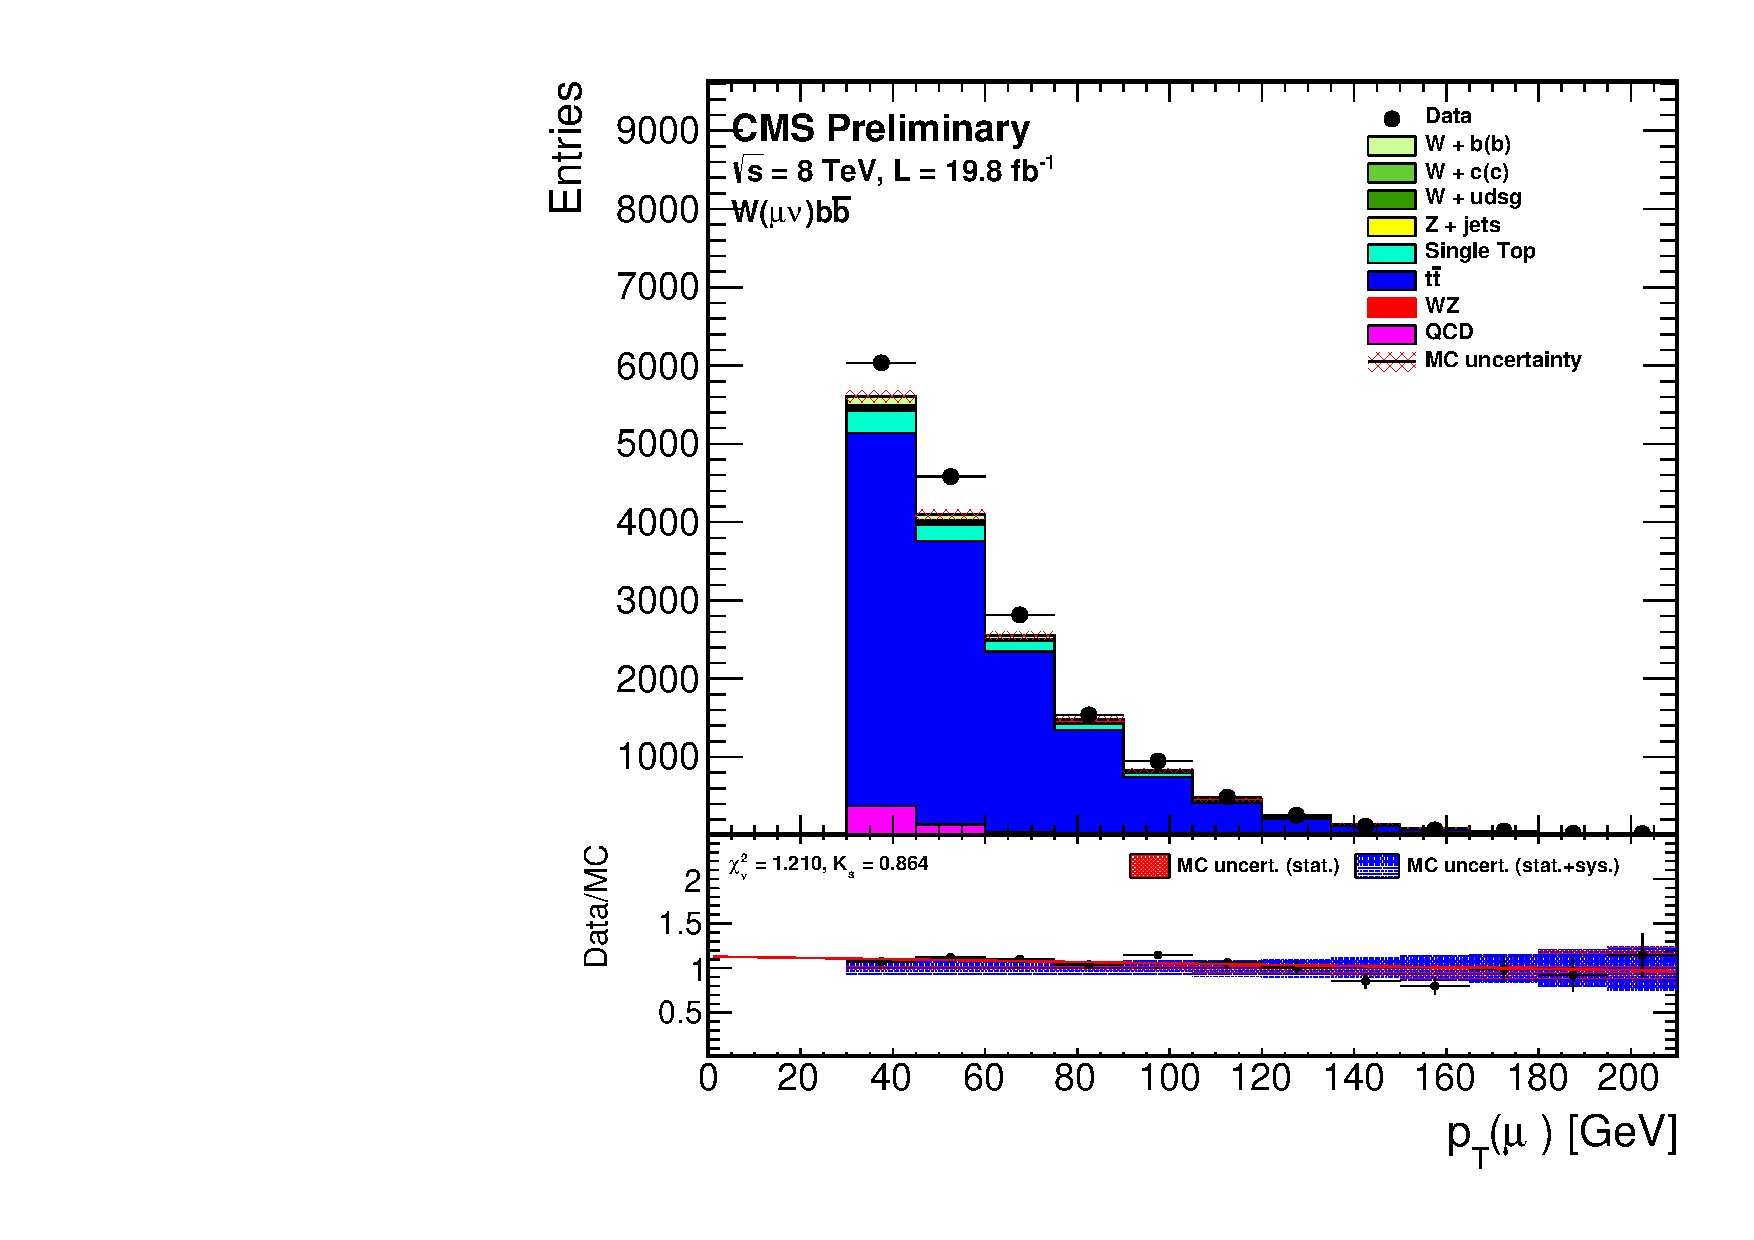
\includegraphics[width=0.48\textwidth]{Figures/Results/Muon/prefit/TT_vLepton_pt_doQCD1.pdf}
		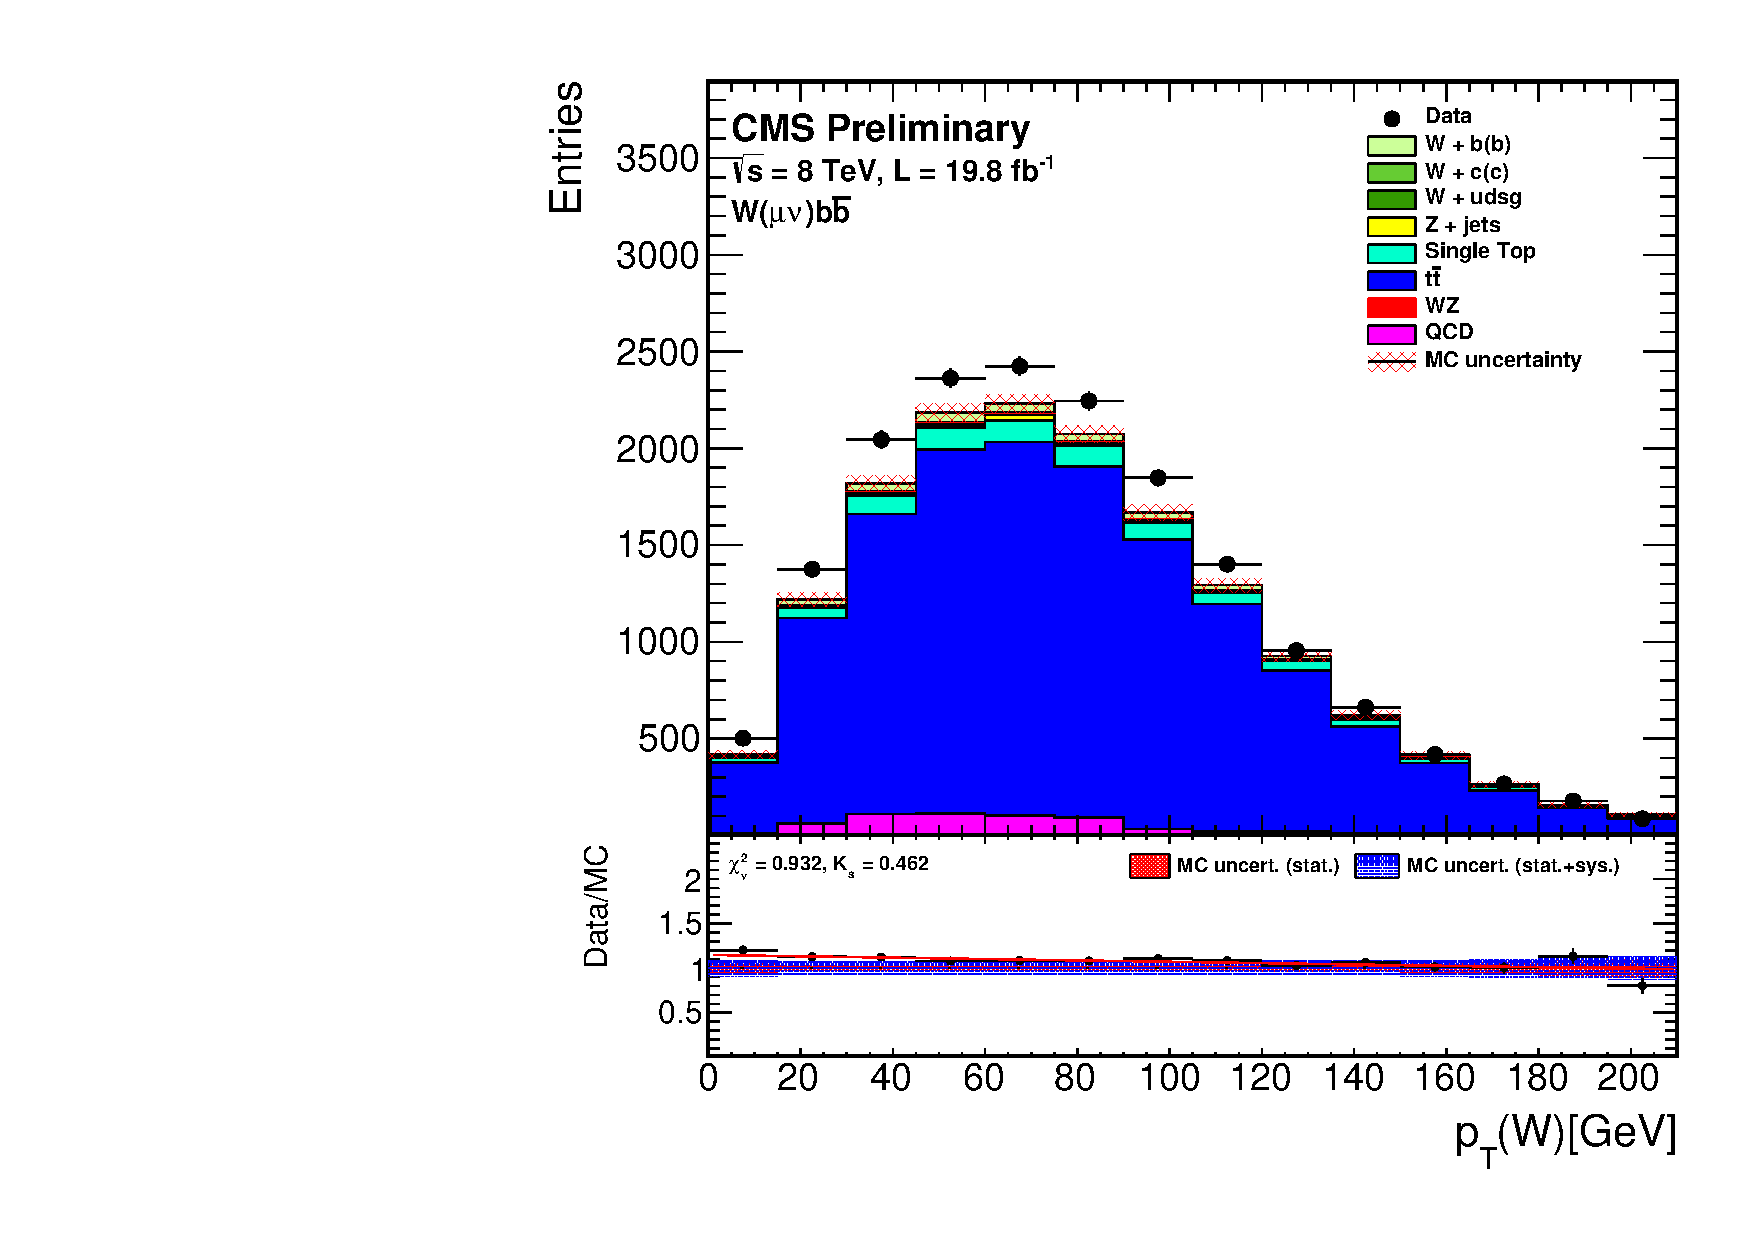
\includegraphics[width=0.48\textwidth]{Figures/Results/Muon/prefit/TT_GetWpt_doQCD1.pdf}
		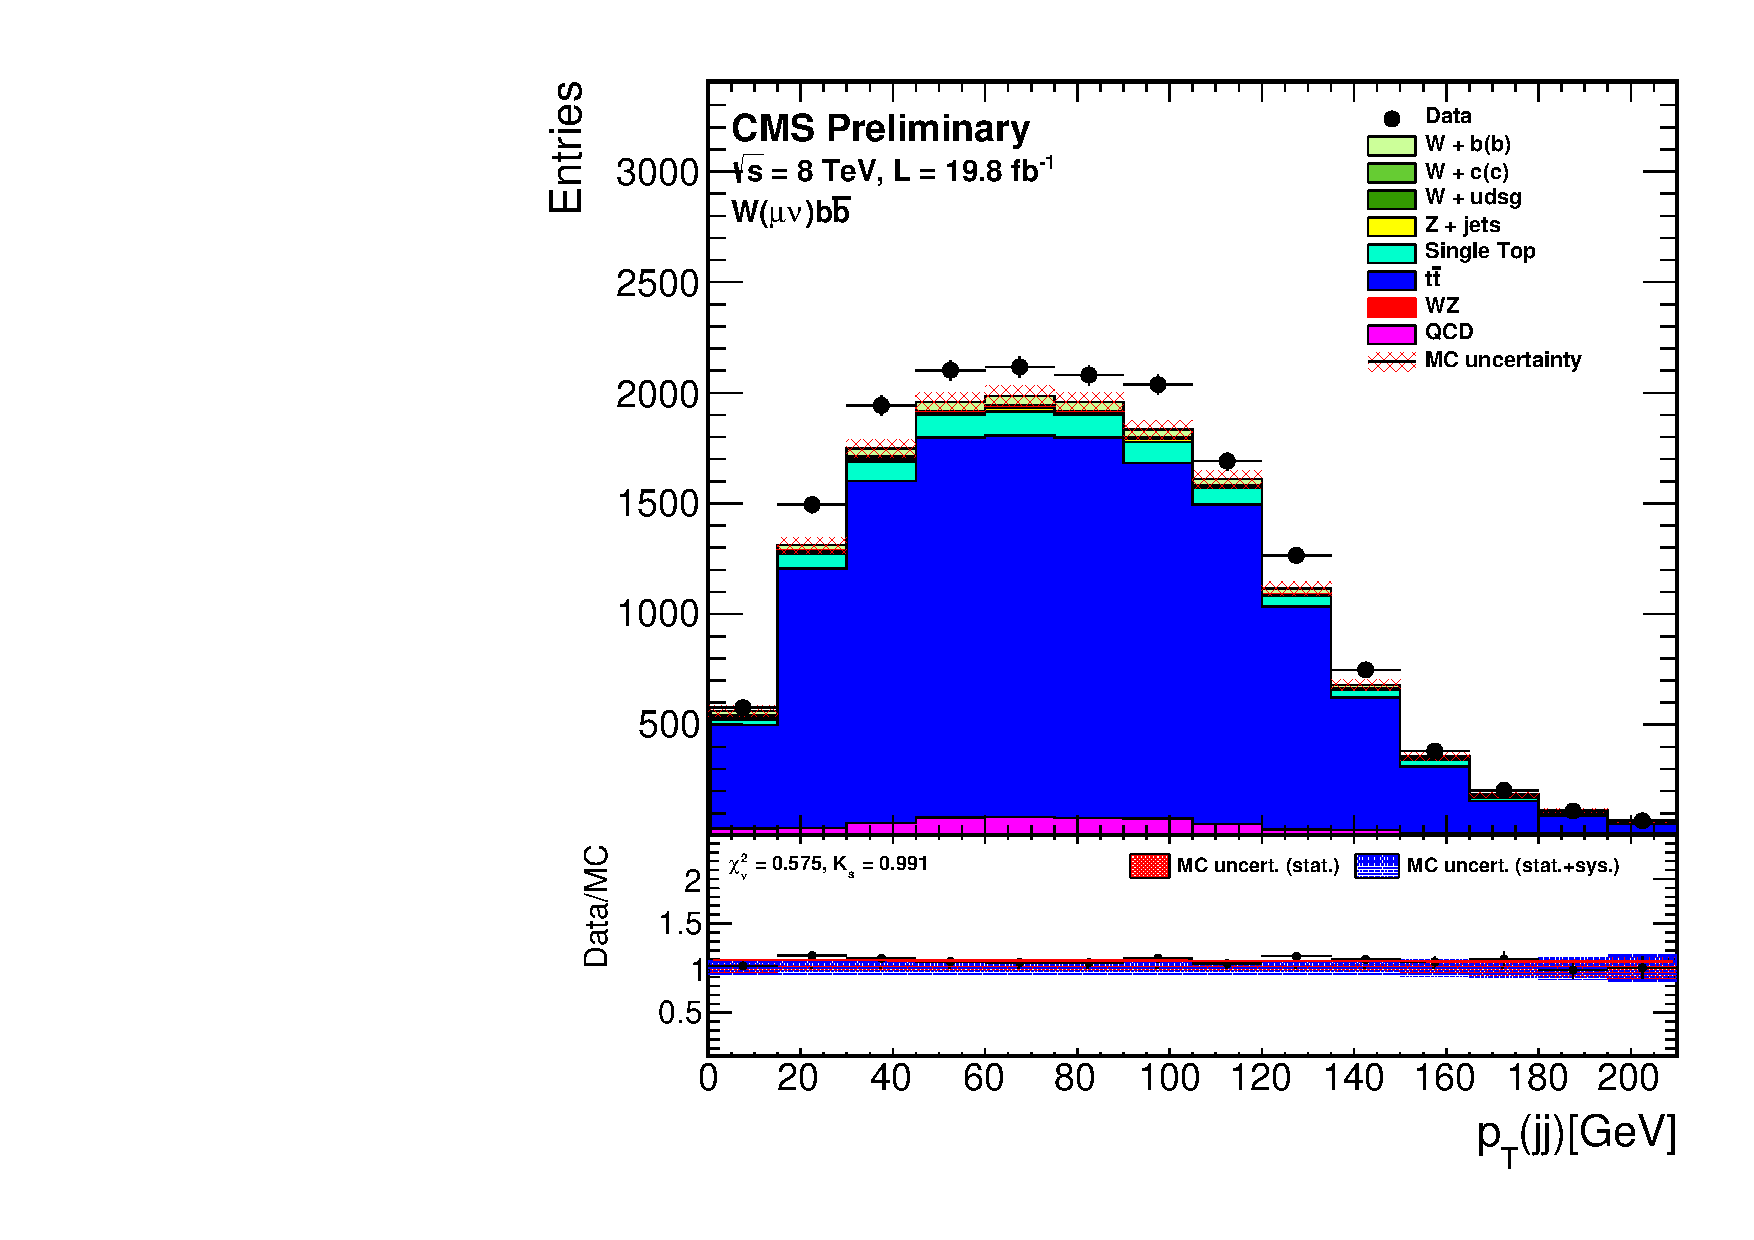
\includegraphics[width=0.48\textwidth]{Figures/Results/Muon/prefit/TT_H_pt_doQCD1.pdf}
		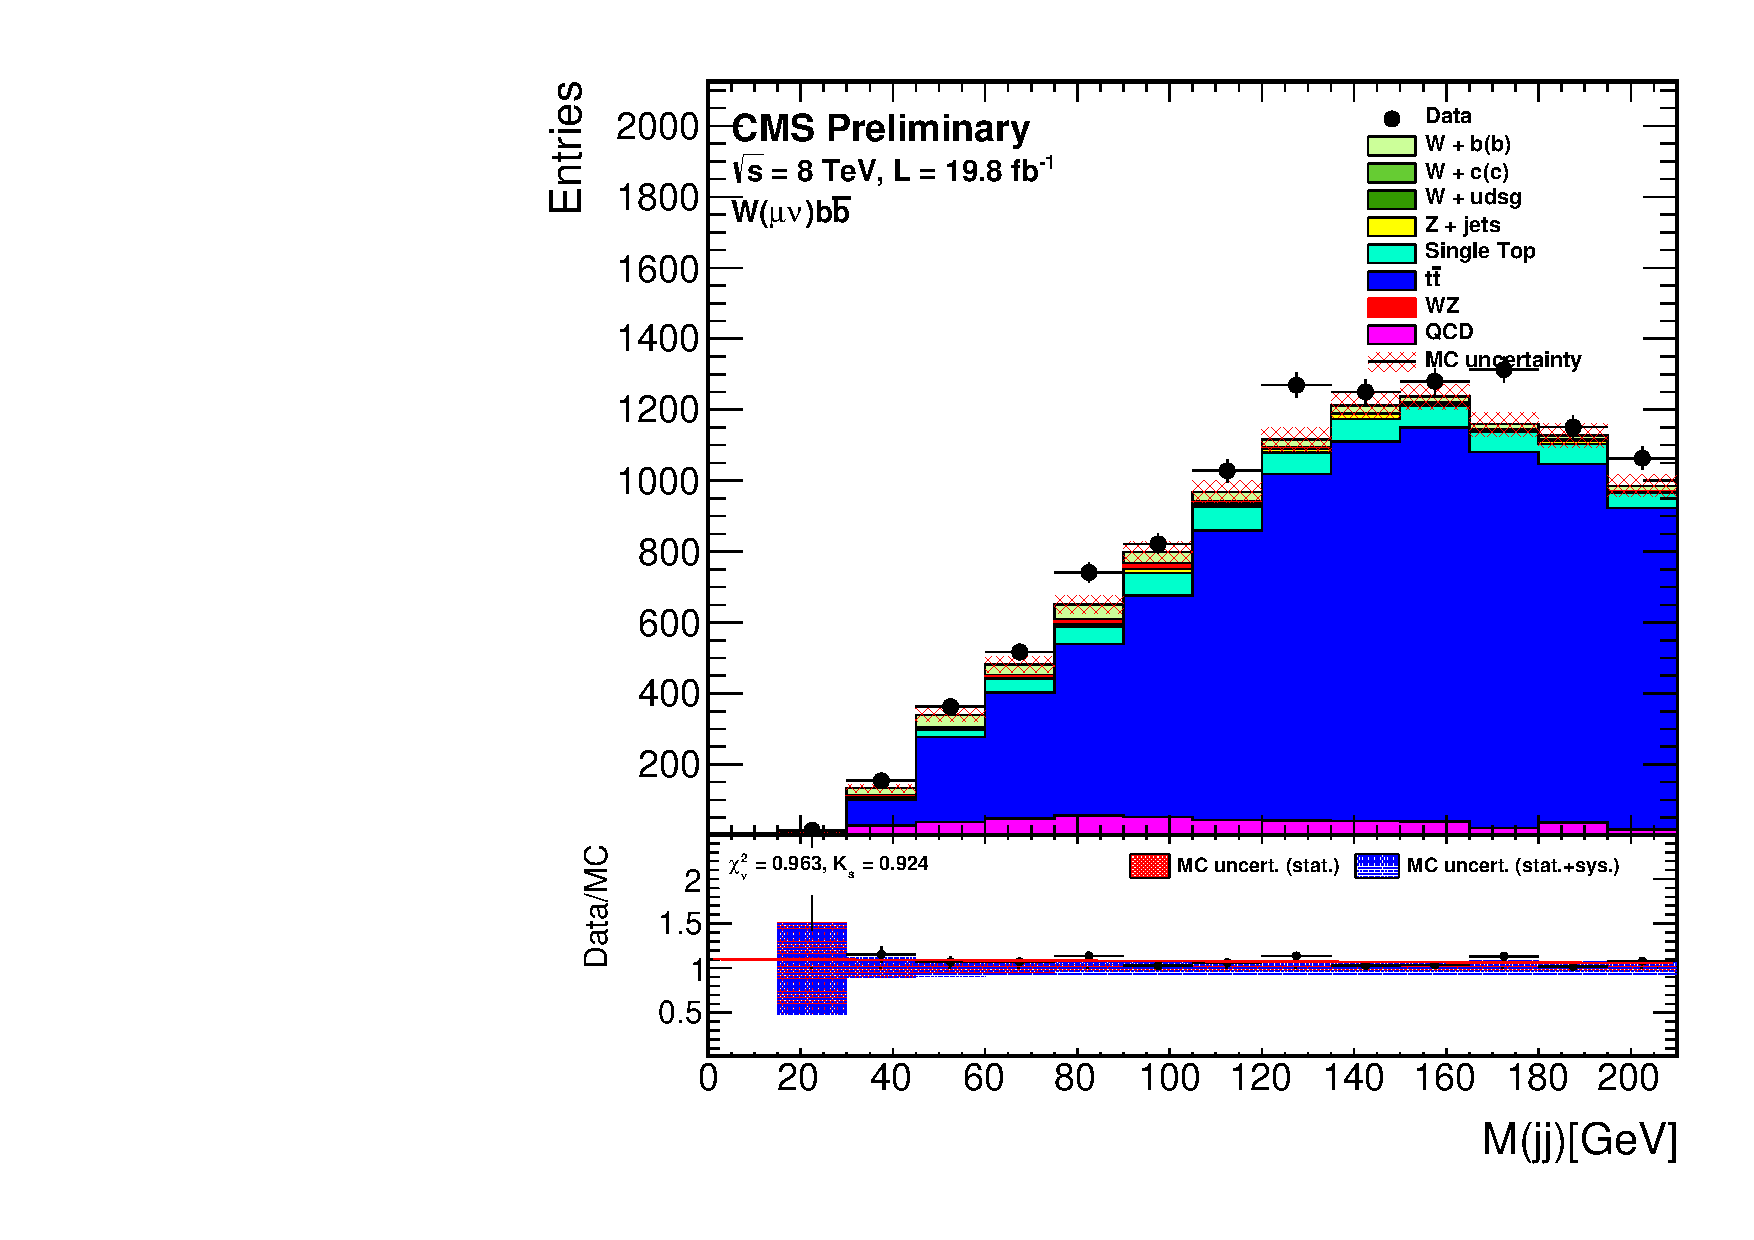
\includegraphics[width=0.48\textwidth]{Figures/Results/Muon/prefit/TT_H_mass_doQCD1.pdf}
		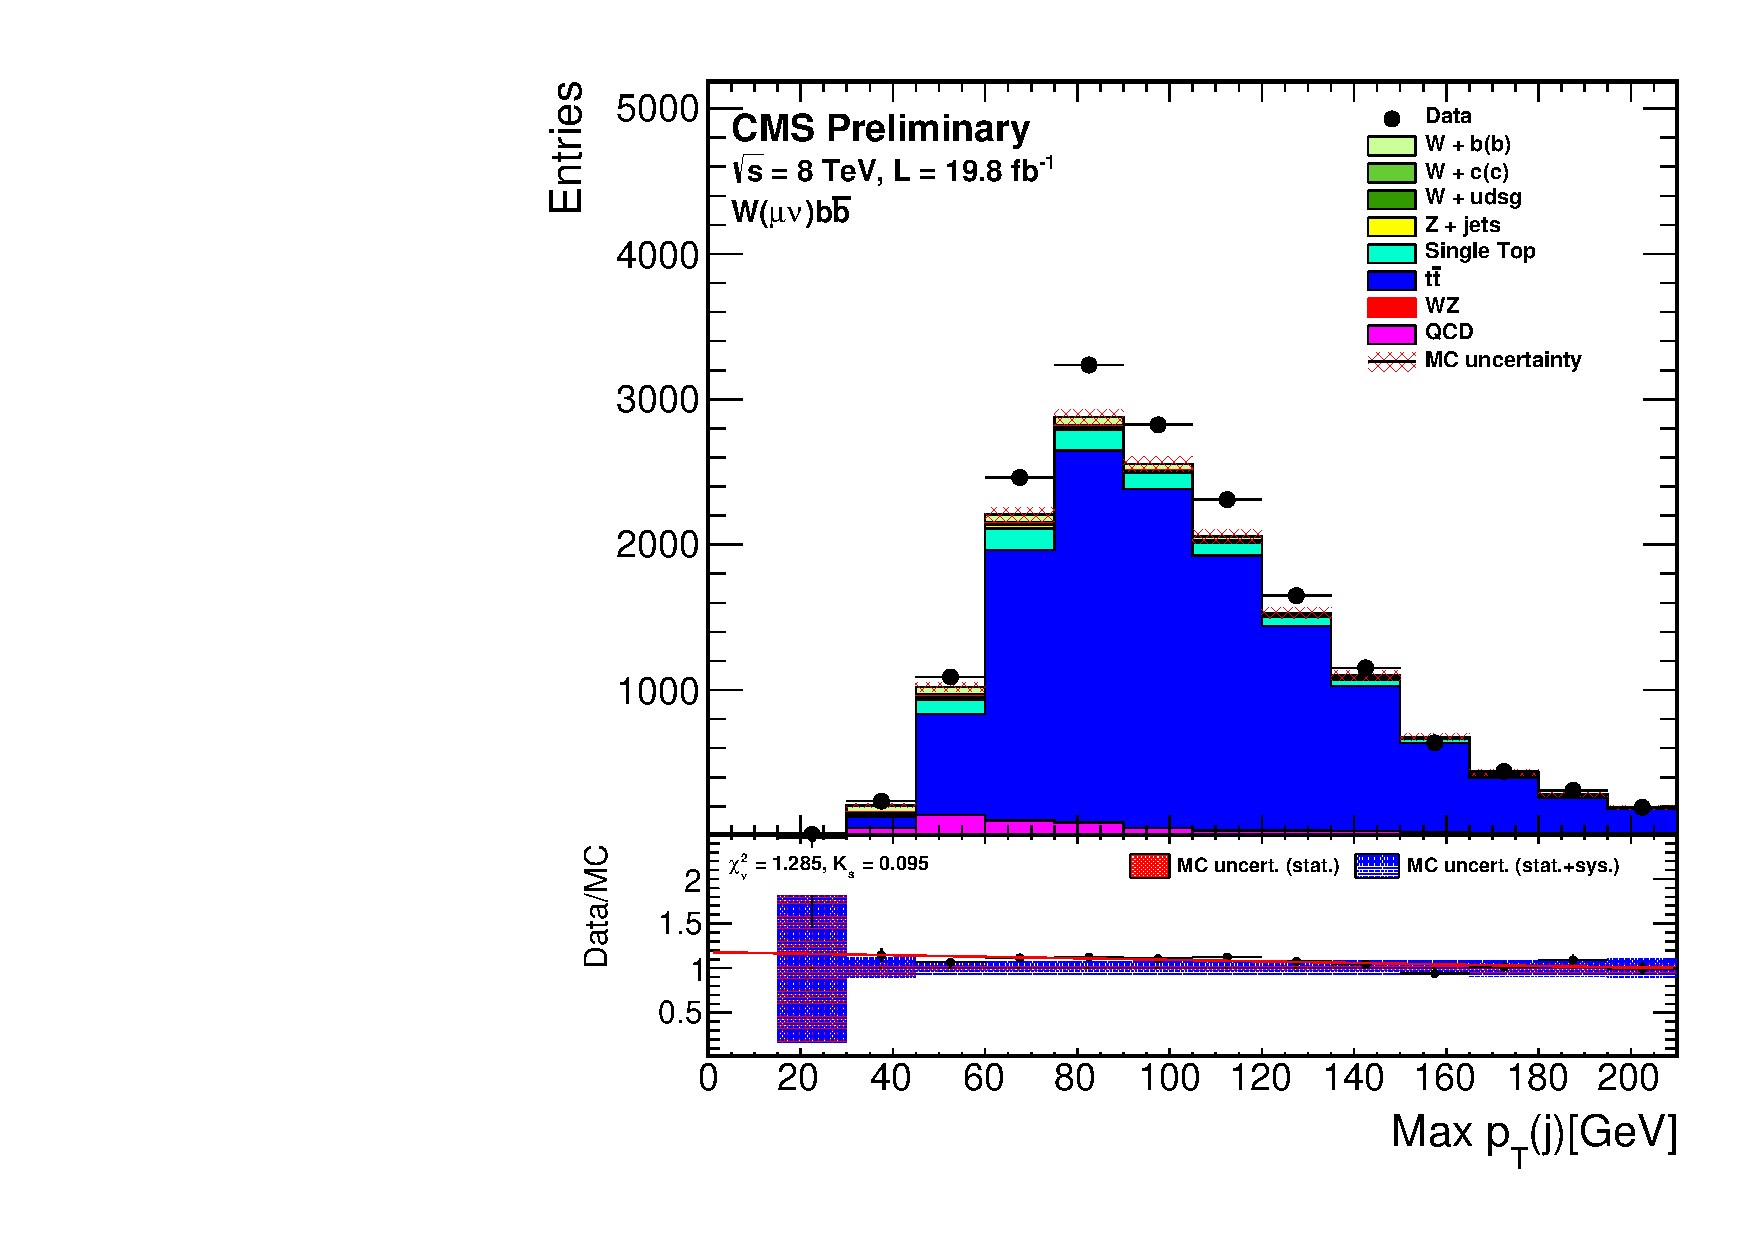
\includegraphics[width=0.48\textwidth]{Figures/Results/Muon/prefit/TT_max_hJet_pt_doQCD1.pdf}		
		%\rule{35em}{0.5pt}
	\caption[Top quark control region]{Various top quark control region distributions: missing energy, lepton transverse momentum, W transverse momentum, invariant mass and transverse momentum of two b jets and highest jet transverse momentum. Good shape agreement between data and simulation is observed, however simulation normalization is smaller than expected from data.}
	\label{fig:TT_CR}
\end{figure}

\subsection{Z+jets}

The contribution from the events where Z boson is produced in association with two b jets is largely suppressed by requiring only one lepton in the event. However, it can happen that one of the leptons from Z decay escapes the detection or is missidentified which possibly causes significant missing energy. Such events are than passing all selection criteria and have to be taken into account in the final cross section measurement. 

\subsection{W+light jets and W+charm}

W+jets is the major background before applying the b-tagging criteria is visible in figure \ref{fig:Wjets}. Both shape and normalization agree well between data and Monte Carlo for several distributions shown. Very tight b-tag selection reduces both W+light jets and W+charm to almost negligible levels.  

\begin{figure}[htbp]
	\centering
		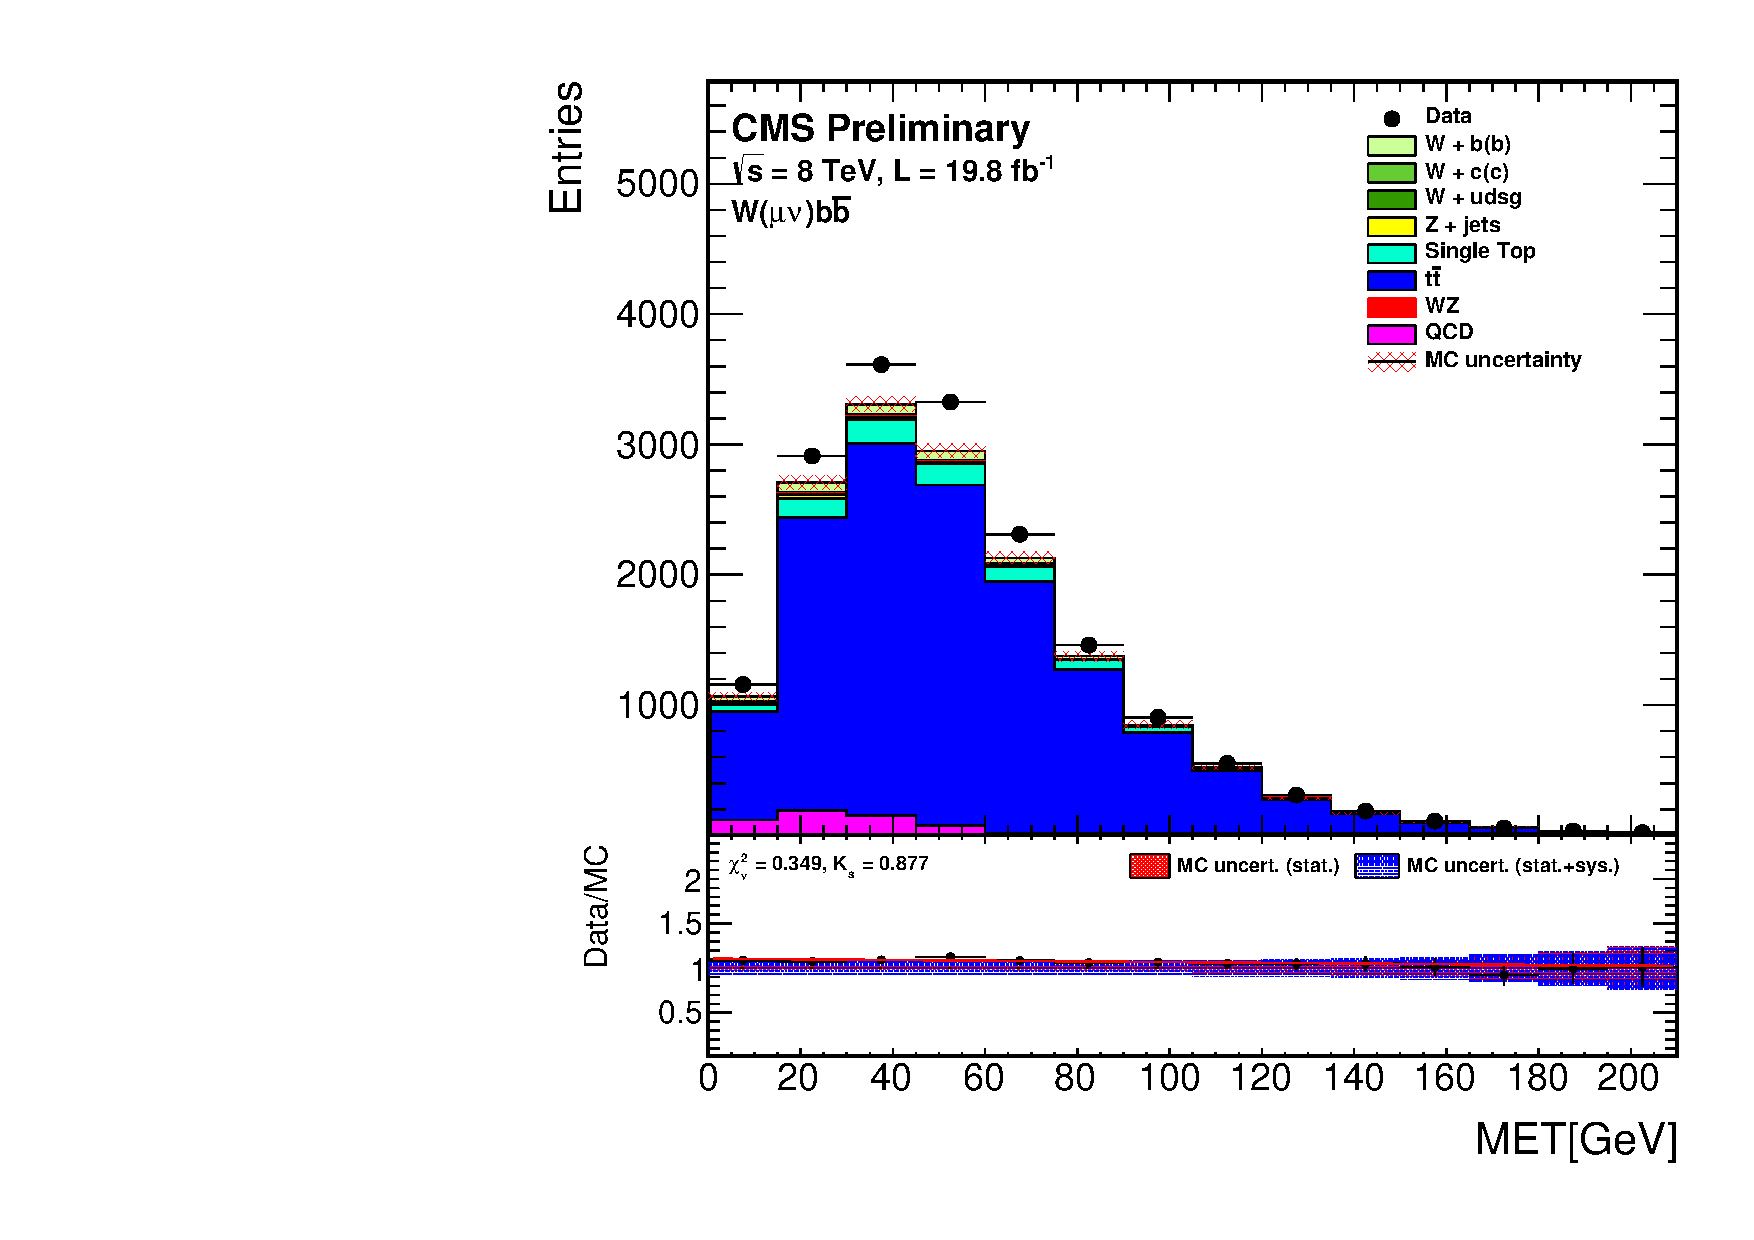
\includegraphics[width=0.48\textwidth]{Figures/Results/Muon/prefit/TT_GetMET_doQCD1.pdf}
		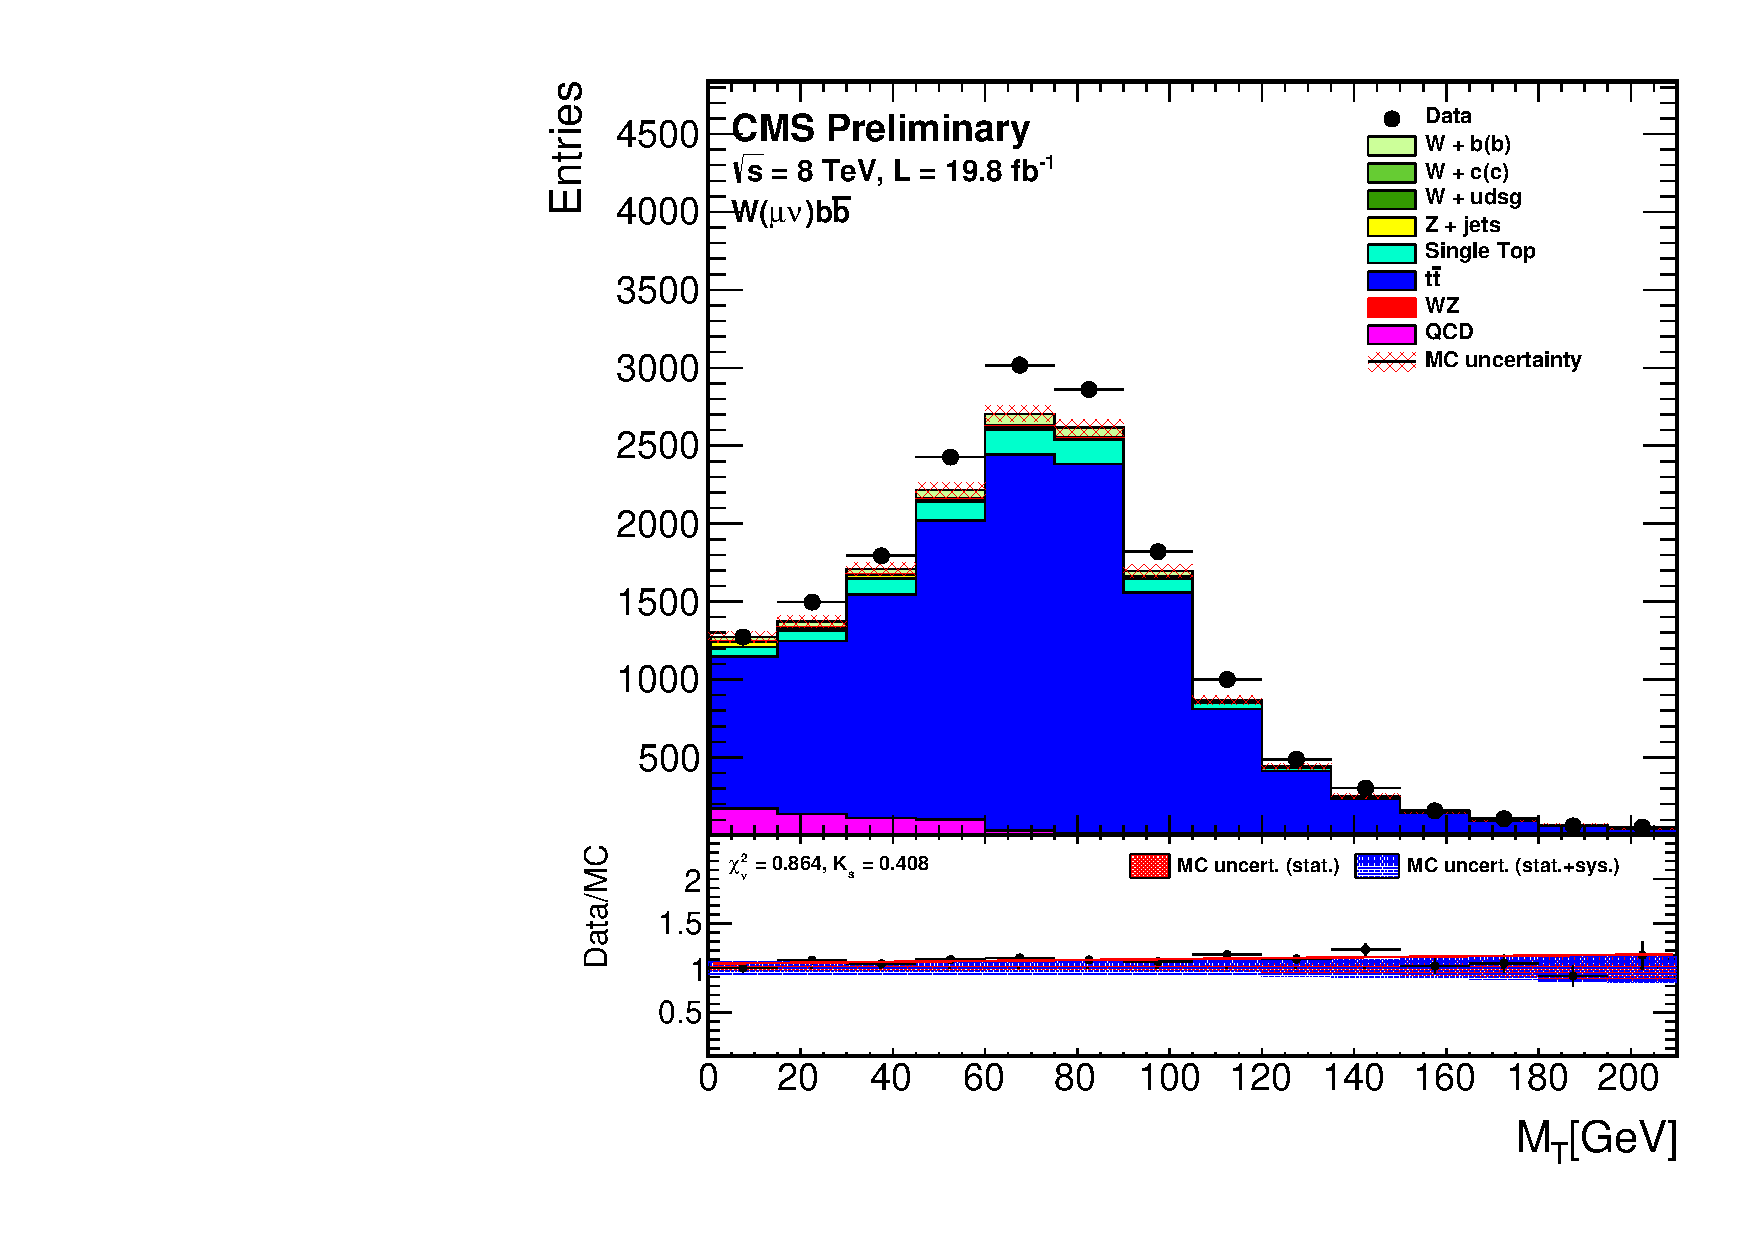
\includegraphics[width=0.48\textwidth]{Figures/Results/Muon/prefit/TT_GetVMt_doQCD1.pdf}
		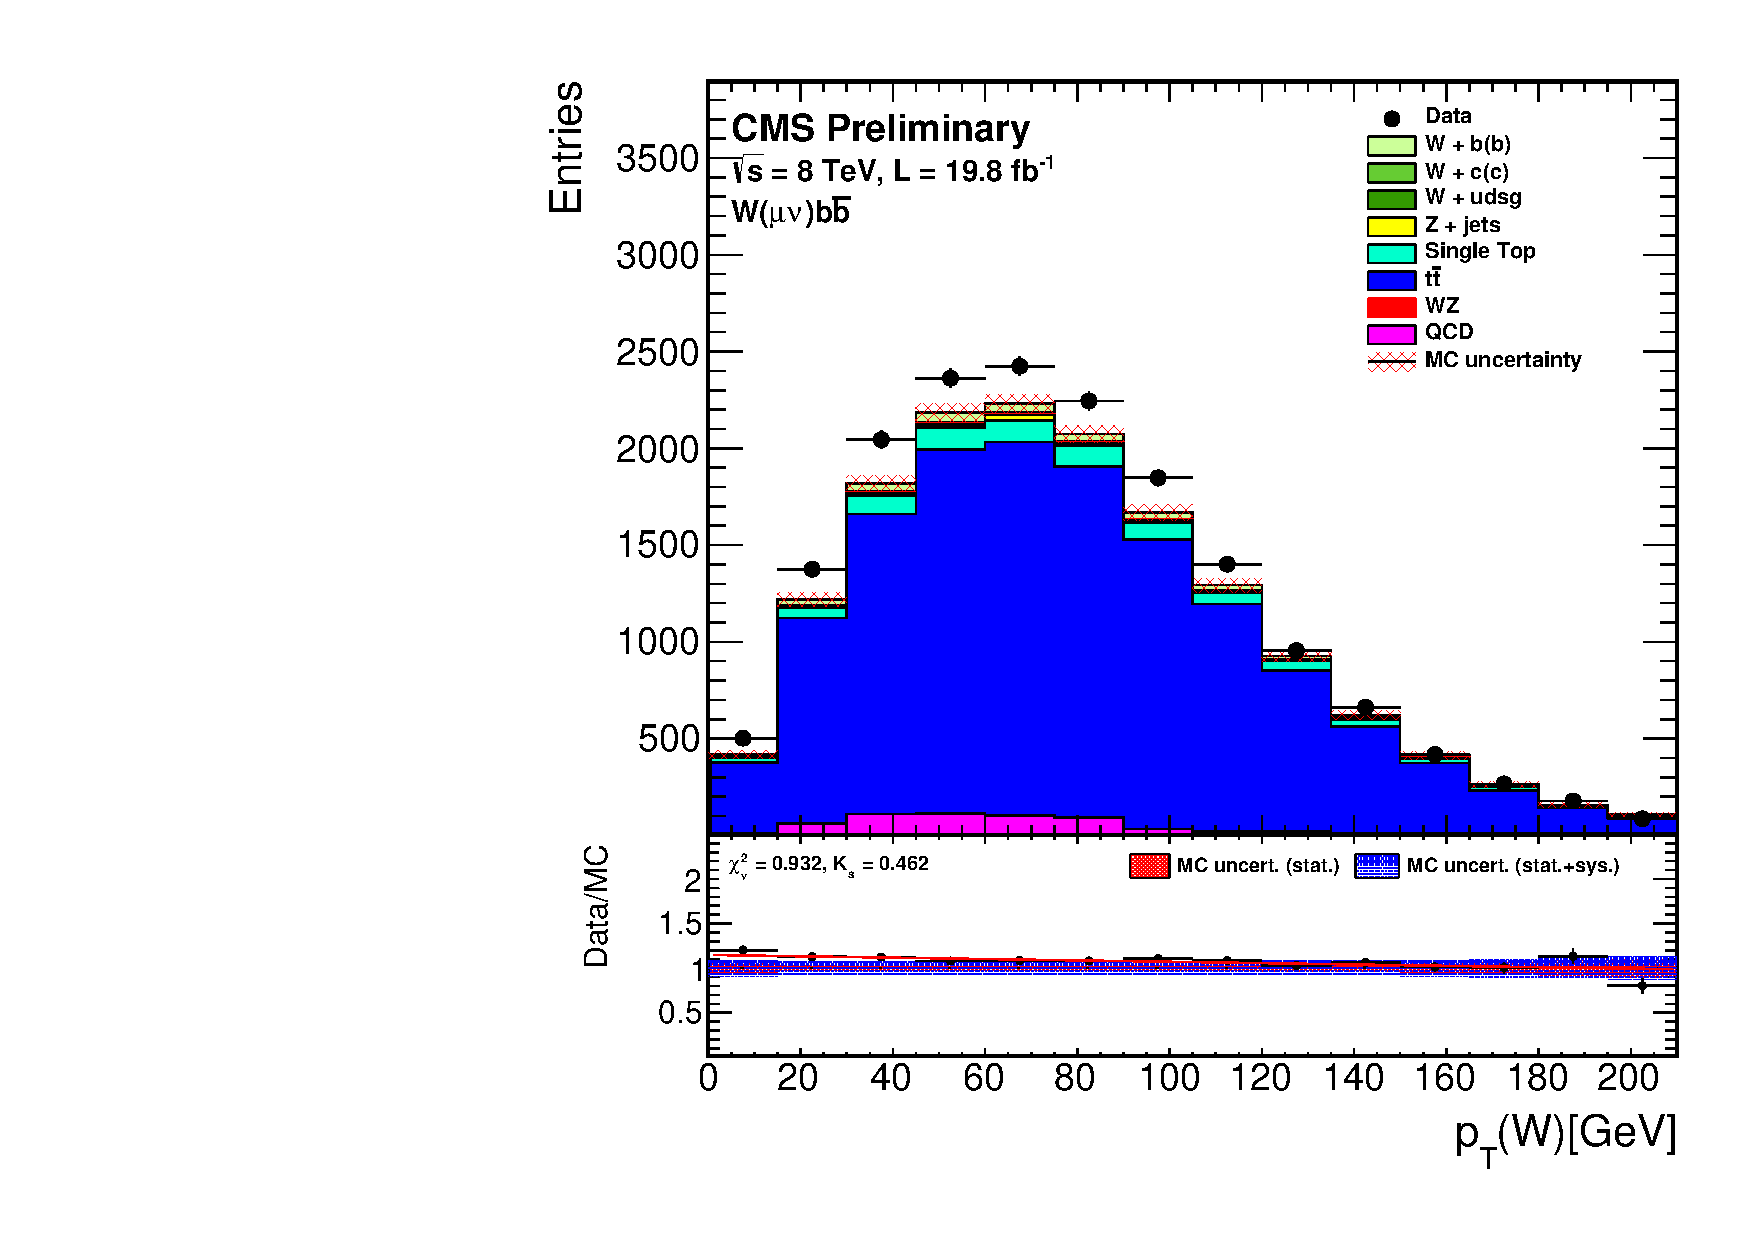
\includegraphics[width=0.48\textwidth]{Figures/Results/Muon/prefit/TT_GetWpt_doQCD1.pdf}
		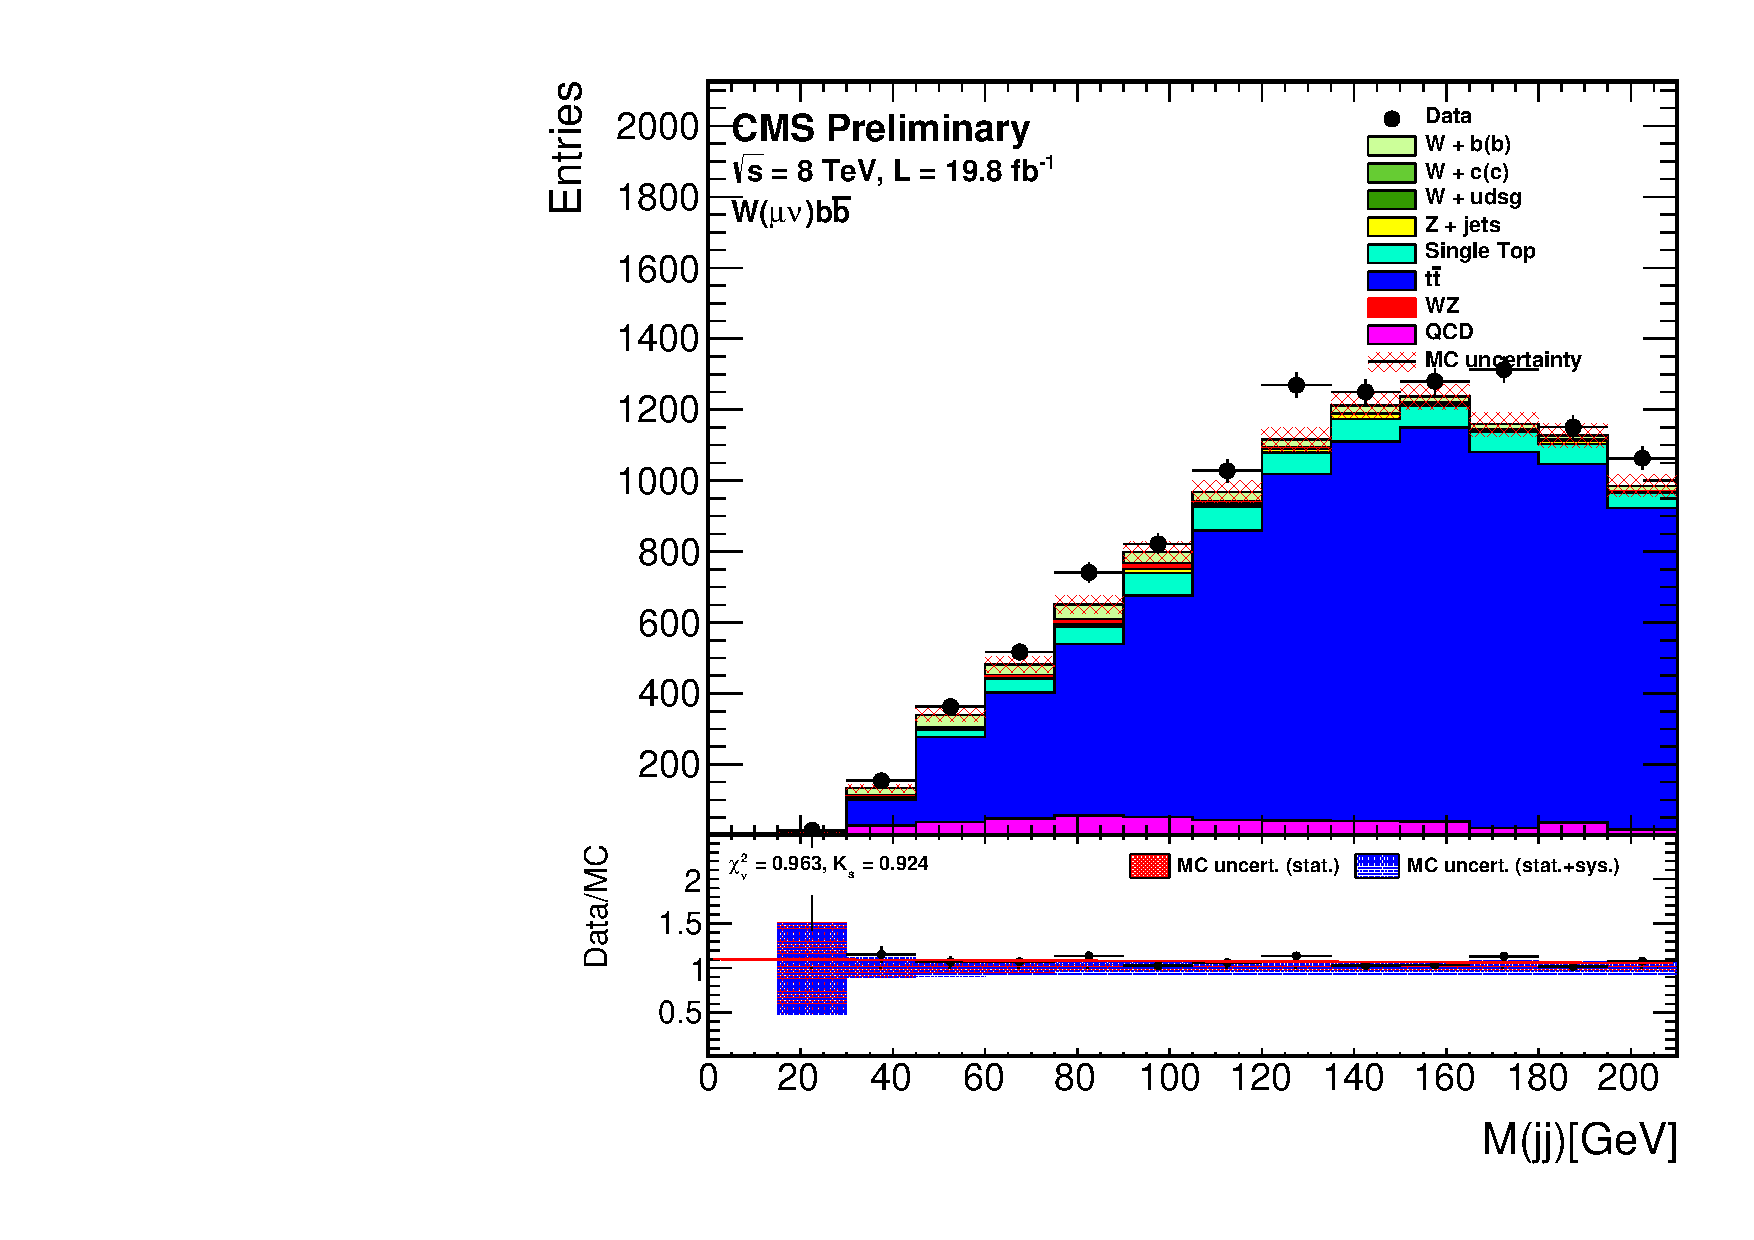
\includegraphics[width=0.48\textwidth]{Figures/Results/Muon/prefit/TT_H_mass_doQCD1.pdf}		
		%\rule{35em}{0.5pt}
	\caption[Distribution obtained using Wbb event selection before applying b-tagging criteria.]{PLACEHOLDER - Distribution obtained using Wbb event selection before applying b-tagging criteria.}
	\label{fig:Wjets}
\end{figure}

\subsection{QCD}
\label{sec:QCD}

QCD background arises from QCD multijet events containing soft lepton which passes lepton selection criteria. An example of such event is shown in the left part of figure \ref{fig:QCD}. This is one of the most challenging backgrounds as it is difficult to simulate significant amount of such events without restrictions. Therefore, the contribution of QCD events in the signal region is determined from data. Two uncorrelated variables are chosen, in this case transverse mass and lepton isolation. Transverse mass distribution shows Jakobian peak for the events containing a W boson, thus it is a natural choice for discrimination from the non W boson final states. In the case of QCD multijet, transverse mass distribution at low values is dominated by the such events. The method is illustrated on the right hand side of the figure \ref{fig:QCD}. Signal region is marked with A. Control sample dominated by QCD events is created by inverting the lepton isolation cut to $I_{rel}^{PF}>0.2$ ($0.15$) for muons (electrons) and is marked with C. The rest of the selection criteria in the control sample is the same as in signal region. The obtained sample is relatively clean. Shape of the final distribution is determined by subtracting the simulated background events that pass the selection. 
\par It is assumed that the QCD distribution has the same shape in regions A and C. Normalization of the QCD distribution is determined form the $M_T$ region below 30 GeV (normalizing D region to B region). In these regions, contributions from other simulated events is subtracted from the data before the normalization. The number of QCD events is expressed as:
\begin{equation}
QCD^A=\frac{N^B_{data}-N^B_{MC}}{N^D_{data}-N^D_{MC}}\times QCD^{C}_{data}
\end{equation}       
where $N^B_{data}$ and $N^D_{data}$ are the number of data events in data in regions B and D respectively, and $N^C_{MC}$ and $N^D_{MC}$ are the number of MC background events in regions B and D respectively. The signal region before and after the QCD contribution determination is shown in figure \ref{fig:QCD_dist}.
\begin{figure}[htbp]
	\centering
		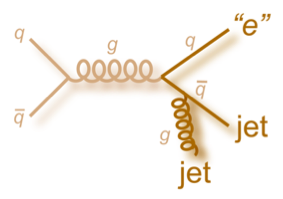
\includegraphics[width=0.4\textwidth]{Figures/QCD_diag.png}
		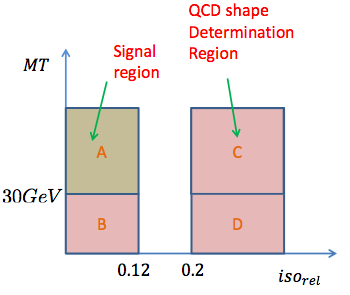
\includegraphics[width=0.45\textwidth]{Figures/QCD_AB.png}		
		%\rule{35em}{0.5pt}
	\caption[QCD diagram and illustration of QCD background determination]{An example of QCD event which looks like signal event (\textit{left}) and illustration of ABCD method used for QCD background determination (\textit{right})}
	\label{fig:QCD}
\end{figure} 

\begin{figure}[htbp]
	\centering
		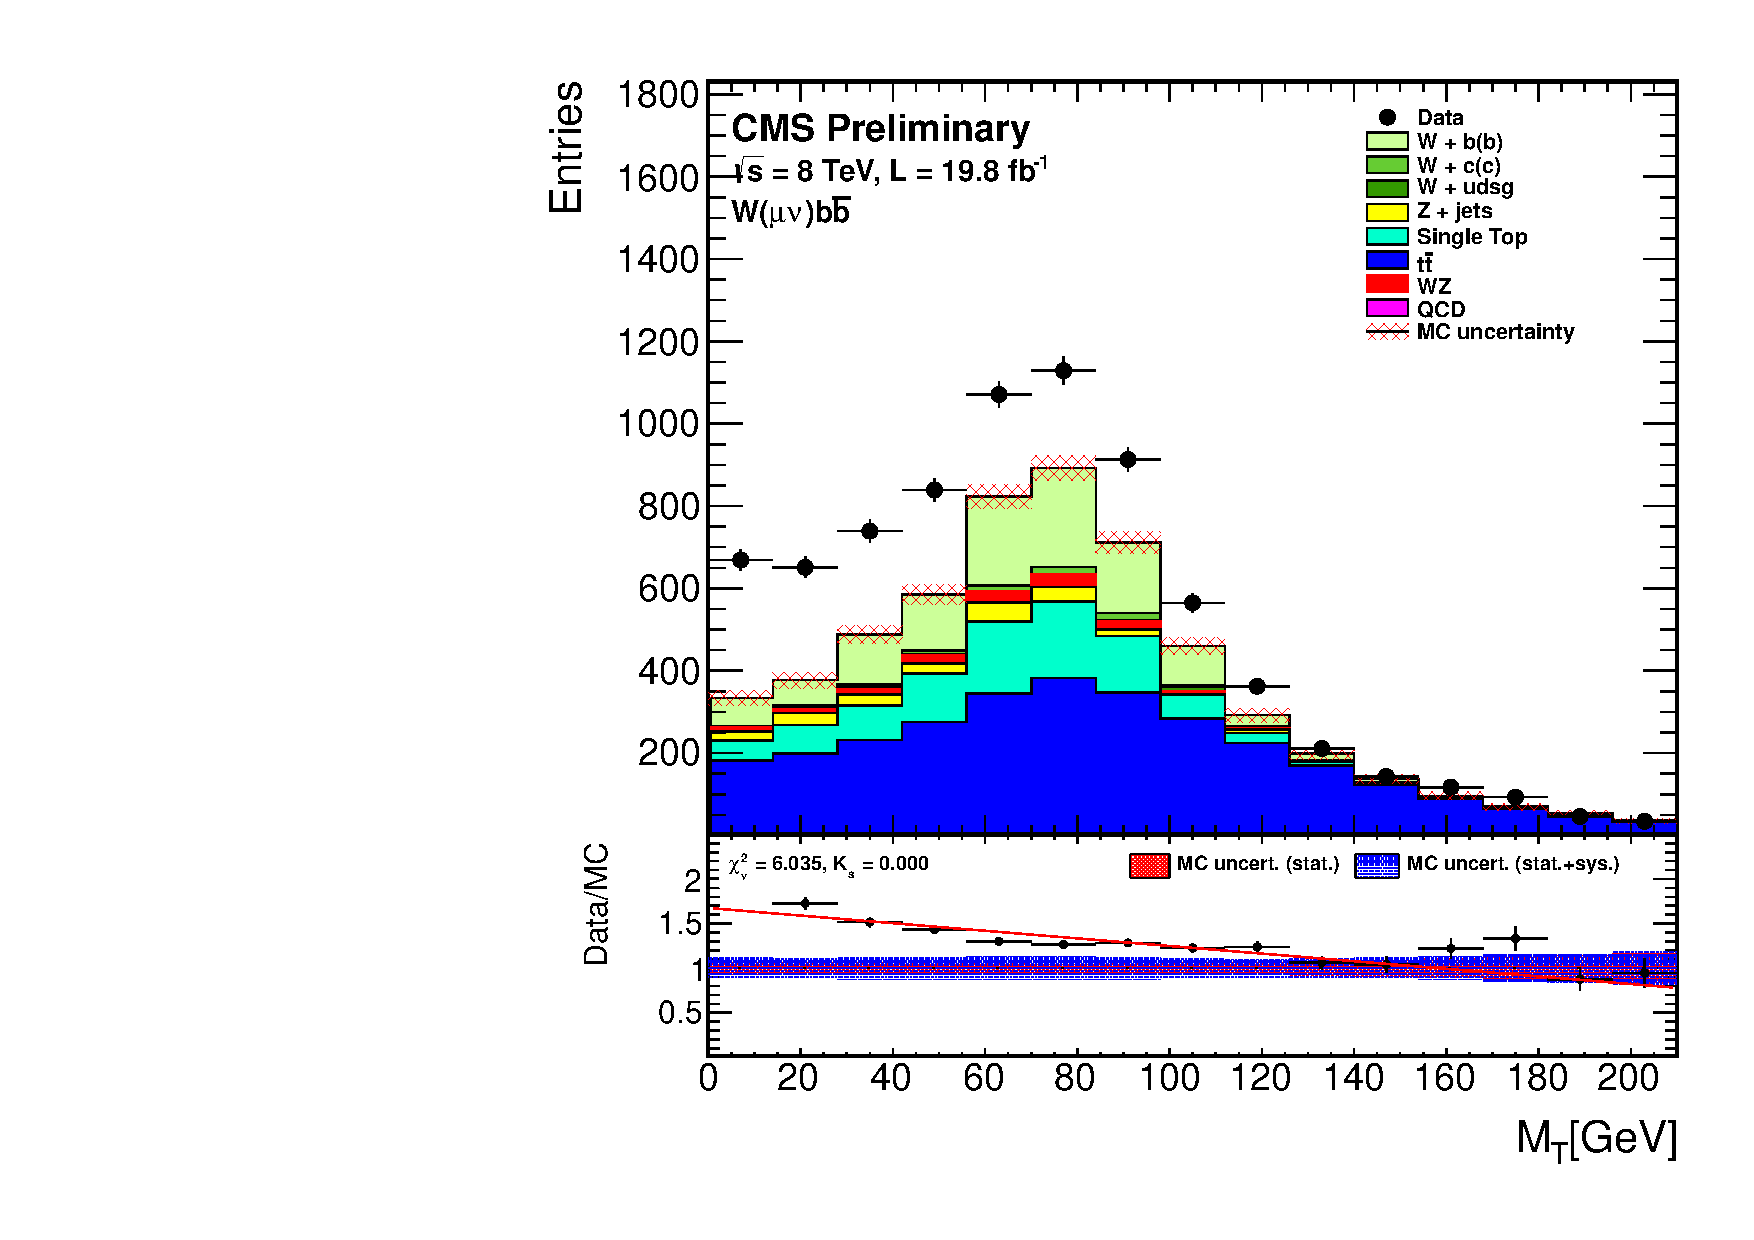
\includegraphics[width=0.48\textwidth]{Figures/VMt_QCD_before.pdf}
		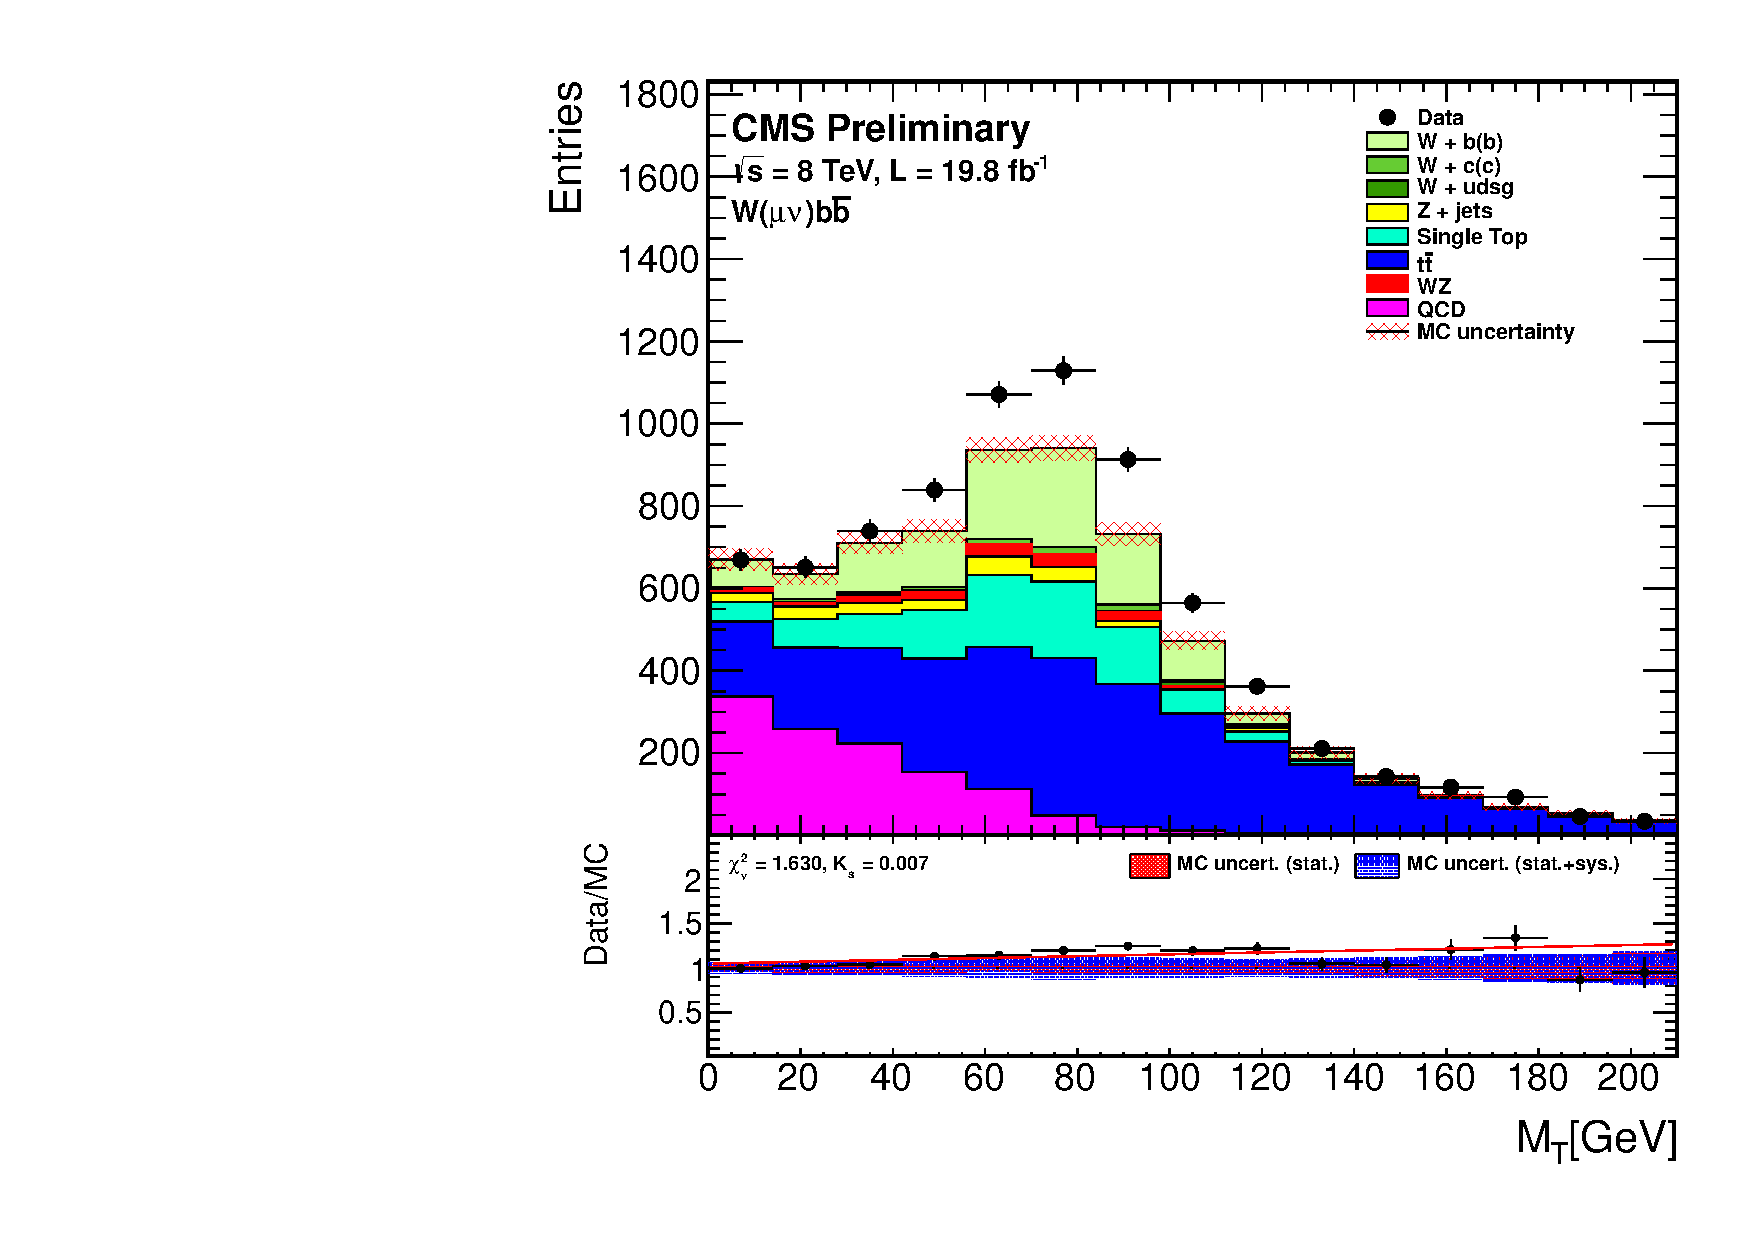
\includegraphics[width=0.48\textwidth]{Figures/VMt_QCD_after.pdf}		
		%\rule{35em}{0.5pt}
	\caption[Transverse mass distribution before and after QCD distribution determination.]{Transverse mass distribution without (\textit{left}) and with QCD background (\textit{right}).}
	\label{fig:QCD_dist}
\end{figure} 


\subsection{Other backgrounds}
Other backgrounds include processes with final states that match the final state of the signal. One of such signals is WZ where W decays leptonically and Z decays in a pair of b quarks. Another example is the production of Higgs boson in association with W boson where Higgs  decays to a pair of b quarks. Such backgrounds are called irreducible backgrounds.


